% !TeX program = lualatex 
\documentclass[ba,logo]{mlai-thesis} 

%%%%%%%%%%%%%%%%%%%%%%%%%%%%%%%%%%%
% Language Settings
%%%%%%%%%%%%%%%%%%%%%%%%%%%%%%%%%%%

% To specify the language of your thesis, uncomment the appropriate setting
% which depends on your LaTeX compiler. If you use a modern compiler such as
% LuaLaTeX or XeLaTeX, it is recommended to use the 'polyglossia' package to
% specify the language. If you use LaTeX or PDFLaTeX, 'babel' is recommended. 

% English

% LuaLaTeX or XeLaTeX 
%\usepackage{polyglossia}
%\setmainlanguage{english} 

% PDFLaTeX 
%\usepackage[english]{babel}

% German 

% LuaLaTeX or XeLaTeX 
\usepackage{polyglossia}
\setmainlanguage{german} 

% PDFLaTeX 
%\usepackage[ngerman]{babel}

\usepackage{algorithm}
\usepackage[noend]{algpseudocode}

%%%%%%%%%%%%%%%%%%%%%%%%%%%%%%%%%%%
% Settings for list environments 
%%%%%%%%%%%%%%%%%%%%%%%%%%%%%%%%%%%

\usepackage{enumitem}

\setlist{nosep,topsep=1ex,labelindent=\parindent,listparindent=\parindent}

\setlist[description]{leftmargin=2cm,style=nextline}

\setlist[enumerate,1]{label=(\roman*)}
\setlist[enumerate,2]{label=(\alph*)}
\setlist[enumerate,3]{label=(\arabic*)} 

\setlist[itemize,1]{label=\textbullet}
\setlist[itemize,2]{label=\rule[.2ex]{0.8ex}{0.8ex}}
\setlist[itemize,3]{label=-}

%%%%%%%%%%%%%%%%%%%%%%%%%%%%%%%%%%%
% Useful Packages and Settings 
%%%%%%%%%%%%%%%%%%%%%%%%%%%%%%%%%%%

%\usepackage{subcaption}
\usepackage{stackengine}
\usepackage{csquotes}
\usepackage{multirow}
\usepackage{tikz}
\usepackage{pgfplots}
\pgfplotsset{compat=1.17}
\pgfplotsset{every axis/.append style={very thick}}

\usepackage{stmaryrd}
\SetSymbolFont{stmry}{bold}{U}{stmry}{m}{n}

% These are only for development
%\usepackage{todonotes}
%\setlength{\marginparwidth}{2cm}
%\usepackage{comment}
%\excludecomment{figure}
%\let\endfigure\relax
%\excludecomment{table}
%\let\endtable\relax

%%%%%%%%%%%%%%%%%%%%%%%%%%%%%%%%%%%
% Citation Package
%%%%%%%%%%%%%%%%%%%%%%%%%%%%%%%%%%%
\usepackage{varioref}
\usepackage{cleveref}
\usepackage[backend=biber,style=authoryear]{biblatex}
\renewcommand*{\nameyeardelim}{\addcomma\space} 


%%%%%%%%%%%%%%%%%%%%%%%%%%%%%%%%%%%%
% Theoremstyles
%%%%%%%%%%%%%%%%%%%%%%%%%%%%%%%%%%%%
\theoremstyle{break}
\theorembodyfont{\normalfont}
\theoremseparator{.}
\theorempreskip{1em}
\theorempostskip{1em}
\theoremsymbol{\ensuremath{\diamond}}

\newtheorem{thm}{Theorem}[chapter]
\newtheorem{lem}[thm]{Lemma}
\newtheorem{prop}[thm]{Proposition}
\newtheorem{cor}[thm]{Corollary}

\newtheorem{exa}[thm]{Example}
\newtheorem{exas}[thm]{Examples}

\newtheorem{prblm}[thm]{Problem}
\newtheorem{prblms}[thm]{Problems}

\newtheorem{quest}{Question}
\newtheorem{quests}{Questions}

\newtheorem{rmk}[thm]{Remark}
\newtheorem{rmks}[thm]{Remarks}

\newtheorem{defn}[thm]{Definition}

\theoremstyle{nonumberplain}
\theoremheaderfont{\itshape}
\theoremsymbol{\rule{1ex}{1ex}}

\newtheorem{proof}{Proof}

%%%%%%%%%%%%%%%%%%%%%%%%%%%%%%%%%%%%
% Mathematical symbols and shortcuts
%%%%%%%%%%%%%%%%%%%%%%%%%%%%%%%%%%%%

\usepackage{amssymb}   % for more mathematical symbols
\usepackage{amsfonts}
\usepackage{stmaryrd}  % for more mathematical symbols
\usepackage{latexsym}  % for more mathematical symbols,
\usepackage{amsxtra}   % for accents as superscripts
\usepackage{amstext}   % for text in formulas, accents, etc.
\usepackage{bm}        % boldface for non-latin letters
\usepackage{listings}  % for code environments

%%%%%%%%%%%%%%%%%%%%%%%%%%%%%%%%%%%%%%%%%%%%%%%%%%%%%%%%%%%%%%%%
% mathematical bold

\newcommand{\mb}[1]{\mathbb{#1}}

\newcommand{\bA}{\mathbb{A}}
\newcommand{\bB}{\mathbb{B}}
\newcommand{\bC}{\mathbb{C}}
\newcommand{\bD}{\mathbb{D}}
\newcommand{\bE}{\mathbb{E}}
\newcommand{\bF}{\mathbb{F}}
\newcommand{\bG}{\mathbb{G}}
\newcommand{\bH}{\mathbb{H}}
\newcommand{\bI}{\mathbb{I}}
\newcommand{\bJ}{\mathbb{J}}
\newcommand{\bK}{\mathbb{K}}
\newcommand{\bL}{\mathbb{L}}
\newcommand{\bM}{\mathbb{M}}
\newcommand{\bN}{\mathbb{N}}
\newcommand{\bO}{\mathbb{O}}
\newcommand{\bP}{\mathbb{P}}
\newcommand{\bQ}{\mathbb{Q}}
\newcommand{\bR}{\mathbb{R}}
\newcommand{\bS}{\mathbb{S}}
\newcommand{\bT}{\mathbb{T}}
\newcommand{\bU}{\mathbb{U}}
\newcommand{\bV}{\mathbb{V}}
\newcommand{\bW}{\mathbb{W}}
\newcommand{\bX}{\mathbb{X}}
\newcommand{\bY}{\mathbb{Y}}
\newcommand{\bZ}{\mathbb{Z}}

%%%%%%%%%%%%%%%%%%%%%%%%%%%%%%%%%%%%%%%%%%%%%%%%%%%%%%%%%%%%%%%%
% mathematical caligraphic

\newcommand{\mc}[1]{\mathcal{#1}}

\newcommand{\cA}{\mathcal{A}}
\newcommand{\cB}{\mathcal{B}}
\newcommand{\cC}{\mathcal{C}}
\newcommand{\cD}{\mathcal{D}}
\newcommand{\cE}{\mathcal{E}}
\newcommand{\cF}{\mathcal{F}}
\newcommand{\cG}{\mathcal{G}}
\newcommand{\cH}{\mathcal{H}}
\newcommand{\cI}{\mathcal{I}}
\newcommand{\cJ}{\mathcal{J}}
\newcommand{\cK}{\mathcal{K}}
\newcommand{\cL}{\mathcal{L}}
\newcommand{\cM}{\mathcal{M}}
\newcommand{\cN}{\mathcal{N}}
\newcommand{\cO}{\mathcal{O}}
\newcommand{\cP}{\mathcal{P}}
\newcommand{\cQ}{\mathcal{Q}}
\newcommand{\cR}{\mathcal{R}}
\newcommand{\cS}{\mathcal{S}}
\newcommand{\cT}{\mathcal{T}}
\newcommand{\cU}{\mathcal{U}}
\newcommand{\cV}{\mathcal{V}}
\newcommand{\cW}{\mathcal{W}}
\newcommand{\cX}{\mathcal{X}}
\newcommand{\cY}{\mathcal{Y}}
\newcommand{\cZ}{\mathcal{Z}}

%%%%%%%%%%%%%%%%%%%%%%%%%%%%%%%%%%%%%%%%%%%%%%%%%%%%%%%%%%%%%%%%
% mathematical fraktur

\newcommand{\mf}[1]{\mathfrak{#1}}

\newcommand{\fA}{\mathfrak{A}}
\newcommand{\fB}{\mathfrak{B}}
\newcommand{\fC}{\mathfrak{C}}
\newcommand{\fD}{\mathfrak{D}}
\newcommand{\fE}{\mathfrak{E}}
\newcommand{\fF}{\mathfrak{F}}
\newcommand{\fG}{\mathfrak{G}}
\newcommand{\fH}{\mathfrak{H}}
\newcommand{\fI}{\mathfrak{I}}
\newcommand{\fJ}{\mathfrak{J}}
\newcommand{\fK}{\mathfrak{K}}
\newcommand{\fL}{\mathfrak{L}}
\newcommand{\fM}{\mathfrak{M}}
\newcommand{\fN}{\mathfrak{N}}
\newcommand{\fO}{\mathfrak{O}}
\newcommand{\fP}{\mathfrak{P}}
\newcommand{\fQ}{\mathfrak{Q}}
\newcommand{\fR}{\mathfrak{R}}
\newcommand{\fS}{\mathfrak{S}}
\newcommand{\fT}{\mathfrak{T}}
\newcommand{\fU}{\mathfrak{U}}
\newcommand{\fV}{\mathfrak{V}}
\newcommand{\fW}{\mathfrak{W}}
\newcommand{\fX}{\mathfrak{X}}
\newcommand{\fY}{\mathfrak{Y}}
\newcommand{\fZ}{\mathfrak{Z}}

%%%%%%%%%%%%%%%%%%%%%%%%%%%%%%%%%%%%%%%%%%%%%%%%%%%%%%%%%%%%%%%%
% math operators
\DeclareMathOperator{\Spur}{Spur}

%%%%%%%%%%%%%%%%%%%%%%%%%%%%%%%%%%%%%%%%%%%%%%%%%%%%%%%%%%%%%%%%
% other math commands

\renewcommand{\bar}[1]{\overline{#1}}
\renewcommand{\hat}[1]{\widehat{#1}}
\newcommand\ddfrac[2]{\frac{\displaystyle #1}{\displaystyle #2}}

%%%%%%%%%%%%%%%%%%%%%%%%%%%%%%%%%%%%%%%%%%%%%%%%%%%%%%%%%%%%%%%%




\title{Data Augmentation mit Variational Autoencodern} 
\author{Paul Henri Iser\\\birthinfo{02. Oktober 1998 in Bonn, Deutschland}}

\thesistype{Bachelorarbeit} 
\examiner{
  Dr. Pascal Welke\\Universität Bonn \and
  Prof. Dr. Christian Bauckhage\\Universität Bonn
}
\supervisor{Florian Seiffarth\\Universität Bonn}

\addbibresource{references.bib}

\begin{document}	
	\frontmatter
	
	

	
	\maketitle 
	\cleardoublepage
	
	% Abstract
	\begin{abstract}
  In dieser Arbeit werden verschiedene Data Augmentation Ansätze basierend auf Variational Autoencodern untersucht. Im Fokus stehen die Analyse des erzeugten Latent-Space und die Augmentierung unterschiedlicher Datensätze, wie MNIST, CelebA und PROBEN1. Über reduzierte Varianten dieser Datensätze werden die vorgestellten Methoden auch in Few-Shot Learning Szenarios evaluiert. Die Ergebnisse offenbaren, dass Variational Autoencoder auf kleinen Datenmengen zu einer leichten Verbesserung der Performanz führen. Für größere Datensätze sind die generierten Beispiele jedoch weniger hilfreich. Hier erzielen andere Ansätze, wie Generative-Adversarial-Networks deutlich bessere Ergebnisse. Es wird sich außerdem herausstellen, dass die erzeugten Daten im Fall von Bilddaten eine starke Unschärfe aufweisen. Dennoch bietet der Variational Autoencoder viele Vorteile durch seine Latent-Space Struktur, denn dies erlaubt kontrollierbare Modifikationen der Daten.
\end{abstract}
	\cleardoublepage
	
	% Authorship
	%\chapter*{Statement of Authorship} 
	%I hereby confirm that the work presented in this master thesis has been performed and interpreted solely by myself except where explicitly identified to the contrary. I declare that I have used no other sources and 
aids than those indicated. This work has not been submitted elsewhere in any other form for the fulfillment of any other degree or qualification.

\vspace*{3cm}
\par\noindent%
Bonn, \today \hfill \underline{\hspace*{5.5cm}}
\vspace*{\fill} 
	\chapter*{Eigenst\"{a}ndigkeitserkl\"{a}rung}
	Hiermit versichere ich, dass ich die vorliegende Bachelorarbeit selbstständig und nur unter Verwendung der angegebenen Quellen und Hilfsmittel verfasst habe. 
Die Arbeit wurde bisher in gleicher oder ähnlicher Form keiner anderen Prüfungsbehörde vorgelegt.

\vspace*{3cm}
\par\noindent%
Bonn, \today \hfill \underline{\hspace*{5.5cm}}
\vspace*{\fill}
	\cleardoublepage
	
	% Table of contents
	\tableofcontents
	
	\mainmatter
	
	% Introduction
	\chapter{Einführung}
Neuronale Netzwerke erwiesen sich in den letzten Jahren als eine der mächtigsten Ansätze im Bereich des maschinellen Lernens. Durch immer tiefere Modellarchitekturen konnten auch komplexere Aufgaben gelöst werden (z.B. AlphaFold, \cite{Senior2020}) . Insbesondere für die Aufgabe der Klassifikation dominieren Neuronale Netze den \textit{State-of-the-Art}. Dazu werden üblicherweise große Datenmengen benötigt, welche in vielen Szenarien jedoch nicht zur Verfügung stehen. Im Extremfall sind nur wenige Beispiele pro Klasse vorhanden (\textit{Few-Shot Learning}). Die Gesichtserkennung, wie sie mittlerweile in den meisten modernen Smartphones zu finden ist, stellt ein Beispiel für einen solchen Fall dar. Ein Möglichkeit dieses Problem zu lösen bietet das künstliche Erweitern der gegebenen Daten. \\

Data Augmentation hat sich als eine der Standard Methoden im Umgang mit kleinen oder imbalancierten Datensätzen etabliert. Üblicherweise werden dazu Beispiele aus dem Datensatz über unterschiedliche Transformationen (z.B. Rotation, Translation, Skalierung) augmentiert. Mit Hilfe dieser Methode konnten bemerkenswerte Ergebnisse, insbesondere in der Bildverarbeitung, erzielt werden. Dieser Prozess baut jedoch häufig auf Expertenwissen darüber auf, welche Transformationen für das Erlernen der Aufgabe hilfreich sind. Ohne dieses Expertenwissen können unplausible Beispiele entstehen, welche die Performanz negativ beeinträchtigen. \\

Alternativ bieten Generative Modelle eine effiziente Methode für die automatisierte Erzeugung von Daten. Mittels tiefer konvolutionaler Netzwerk Architekturen wird eine immer bessere Qualität der generierten Daten erreicht. Somit stellen sie inzwischen eine effiziente Alternative zu den klassischen Data Augmentation Methoden dar. Zudem bieten sie den Vorteil, dass im Allgemeinen kein Expertenwissen benötigt wird. So zeigten sie in verschiedensten Bereichen beachtliche Ergebnisse (z.B. GPT-3, \cite{brown2020language}). \\

In der vorliegenden Arbeit wird der Variational Autoencoder (VAE) als generatives Modell betrachtet. Der übliche Nutzen von Autoencodern liegt in einer semantischen Repräsentation der Eingabe. Dies wird über eine Encoder-Decoder Architektur erreicht. Variational Autoencoder erweitern diese Struktur, um eine probabilistische Repräsentation der Eingabe in einem \textit{Latent-Space} zu erzeugen. Diese Arbeit teilt sich in einen theoretischen und einen praktischen Fokus auf. Der theoretische Fokus liegt in der Analyse der Latent-Space Struktur. Insbesondere wird sich mit der Fragestellung beschäftigt, wie diese für die Erzeugung neuer Daten verwendet werden kann. Der praktische Fokus liegt auf der Evaluation verschiedener VAE basierter Data Augmentation Ansätze auf unterschiedlichen Datensätzen. Diese beinhalten sowohl Bild-, als auch numerische Daten. Zudem wird der Einfluss der VAE basierten Ansätze in Few-Shot Szenarien untersucht. Abschließend werden diese Verfahren mit anderen generativen Methoden verglichen.

	
	% Related Work
	\chapter{Wissenschaftlicher Hintergrund}
In den letzten Jahren wurden bereits einige Arbeiten zu der Augmentation von Daten über Generative Modelle veröffentlicht. Einige dieser Arbeiten stellen Konzepte vor, welche auch in dieser Arbeit verwendet werden. Diese werden im Folgenden erläutert.\\

\cite{Jorge2018} untersuchen empirisch, wie die Verwendung von Variational Autoencoder zur Data Augmentation, die Klassifikation auf dem MNIST und Omniglot Datensatz verbessert. Außerdem stellen sie einige Methoden des Latent-Space Samplings vor, welche auch in dieser Arbeit aufgegriffen werden. \cite{Garay-Maestre2019} behandeln zusätzlich die Verbesserungen, die sich auf reduzierten Partitionen von MNIST erzielen lassen. Zudem wird die Verwendung von einem seperaten Modell je Klasse motiviert. Dieser Ansatz wird in der vorliegenden Arbeit aufgegriffen und auf weitere, unter anderem numerische Daten angewendet. \\

\cite{Moreno-Barea2020} beschäftigen sich in ihrer Arbeit mit der Anwendung verschiedener Generativer Modelle auf kleinen Datensätzen. Im Gegensatz zu den anderen Arbeiten in diesem Bereich, werden hier keine Bilddaten untersucht. Stattdessen werden numerische Daten mit teils diskreten Attributen behandelt. Außerdem stellen sie einen Data Augmentation Prozess vor, welcher zusätzlich eine Filterung der generierten Daten nutzt, um unplausible Beispiele auszusortieren. Damit soll die Performanz weiter verbessert werden. Da hier allerdings mehrere Generative Ansätze untersucht werden, macht der Variational Autoencoder nur einen Teil dieser Arbeit aus. Dieser wird in der vorliegenden Arbeit genauer analysiert. \\

\cite{Higgins2017} schlagen eine $\beta$ Erweiterung zum Variational Autoencoder vor, welche die Korrelation erlernter Merkmale beeinflusst. In der Arbeit werden ausschließlich Bilddaten untersucht. Der Fokus der Autoren liegt auf der Qualität der generierten Bilder und der unabhängigen Modifikation von Merkmalen. In der vorliegenden Bachelorarbeit wird darüber hinaus die Auswirkungen auf die Klassifikationsaufgabe für sowohl Bild-, als auch numerische Daten, behandelt. \\

\pagebreak
\cite{goodfellow2014generative} stellen mit "Generative-Adversarial-Networks" eine weitere Architektur eines generativen Modells vor. Diese bietet einige Vorteile gegenüber Variational Autoencodern. Unter anderem werden sehr viel schärfere Bilder generiert, dafür erlauben sie jedoch keine Kontrolle über die generierten Beispiele. Ein Vergleich zu dieser Methode ist einer der zu untersuchenden Aspekte dieser Arbeit.

	
	% Literature
	\chapter{Literatur}
Im Folgenden werden wichtige Begrifflichkeiten und Herleitungen, welche in dieser Arbeit verwendet werden, vorgestellt. Weitere theoretischen Grundlagen zu den vorgestellten Konzepten finden sich in den Arbeiten von \cite{Goodfellow-et-al-2016}, \cite{Kingma2014}.


\section{Few-Shot Learning}
Viele der heutigen \textit{State-of-the-Art} Modelle bauen auf einer riesigen Anzahl von Trainings Beispielen auf. Diese Anforderung kann aber nicht immer erfüllt werden. Bei nur wenig Beispielen ist daher die Gefahr des "Overfittings", d.h. des Auswendig Lernens des Datensatzes, entsprechend groß. Der Forschungsstrang "Few-Shot Learning" beschäftigt sich mit der Aufgabe, eine gute Generalisierung aus nur wenigen Daten zu Erzielen. Für $n$ Trainingsbeispiele pro $k$ Klassen spricht man von $n$-way $k$-shot Learning. \cite{Sung2017} erwähnen "Meta-Learning" als vielversprechenden Ansatz. Dieser geht, nach dem Paradigma "Lernen-zu-lernen" auf die Art zurück, wie Menschen lernen: Kinder haben kein Problem, aus einem einzelnen Bild das Objekt "Zebra" zu verstehen, da sie bereits das Konzept "Pferd" und "Farben" kennen. Kernidee in der von \cite{Sung2017} veröffentlichten Arbeit ist es eine Ähnlichkeitsfunktion zwischen Bildobjekten zu lernen. Realisiert wird dies durch Lernen eines Embedding-Vektors mit dem Ziel, dass ähnliche Objekte in diesem Raum nahe beieinander liegen. So können ungesehene Beispiele über einen "Nearest-Neighbor-Classifier" bekannten Beispielen zugeordnet und klassifiziert werden.

Ein alternativer Ansatz ist die Nutzung von Data Augmentation, um mehr Daten aus den vorhandenen zu erzeugen. Ein Vorteil dieses Weges besteht darin, dass für die Klassifikation wieder auf \textit{State-of-the-Art} Modelle zurückgegriffen werden kann. \cite{Antoniou2017} zeigen, dass auch Generative Modelle dazu verwendet werden können, um Data Augmentation zu betreiben. Mit Hilfe von vielen generierten Daten können gute Generalisierungen erzielt werden.



\section{Autoencoder}\label{sec:autoencoder}
Der Autoencoder (AE) stellt eine Encoder-Decoder Architektur dar (siehe Abb. \ref{fig:ae_model}. Aufgabe des Encoders $f$ ist es, die Eingabe $x$ in einen Merkmalsraum abzubilden. Anschließend versucht der Decoder $g$ die Eingabe zu rekonstruieren. Die Ausgabe des Autoencoders ist somit die Komposition $g(f(x))$. Um eine präzise Rekonstruktion zu erzielen, werden Fehlerfunktionen der folgenden Art verwendet:
\begin{equation}
  \cL(x, g(f(x)))
\end{equation}
Demnach können Autoencoder in einem selbst-überwachten Szenario trainiert werden. Übliche Fehlerfunktionen zur Bewertung der Diskrepanz zwischen $x$ und $g(f(x))$ sind "Binary-Cross-Entropy-Loss" und "Mean-Squared-Error". In Bezug auf die Dimension des Merkmalsraums unterscheidet man zwei Fälle. \\
\begin{figure}[hbt]
\centering
  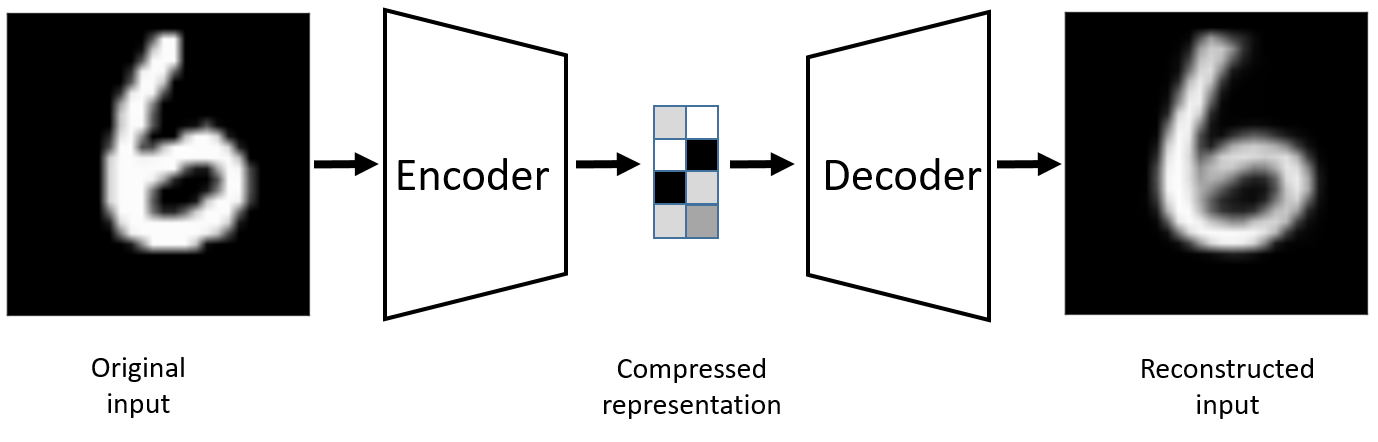
\includegraphics[width=.8\textwidth]{gfx/literature/autoencoder}
  \caption{Die Encoder-Decoder Struktur des "undercomplete" Autoencoders. Der Encoder berechnet eine komprimierte Repräsentation der Eingabe. Der Decoder ist in der Lage diese wieder zu einem Bild zu rekonstruieren. Abb. entnommen aus \cite{LopezPinaya2019}.}
  \label{fig:ae_model}
\end{figure}
Der erste Fall ist der sogenannte "undercomplete" AE. Hierbei wird die Dimension des Merkmalsraums kleiner als die der Eingabe gewählt, sodass dieser einen Flaschenhals für den Informationsfluss bildet. Der Encoder komprimiert die Eingabe und stellt so eine Dimensionsreduktion dar. Falls der Autoencoder $(f \circ g)$ durch eine lineare Abbildung definiert ist, entspricht diese Dimensionsreduktion einer "Principle-Component-Analysis" (PCA) (siehe \cite{ladjal2019pcalike}). Eine Definition über nicht-lineare Abbildungen ist deutlich mächtiger. An dieser Stelle bieten sich Neuronale Netze an, da sie beliebige, insbesondere nicht-lineare Funktionen, approximieren können. Zudem sind (Konvolutionale-) Neurale-Netzwerke (CNN) eine weit verbreitete Methode der automatisierten Merkmalsextraktion. Ein üblicher Nutzen von "undercomplete" Autoencodern ist eben dieser komprimierte Merkmalsvektor als Repräsentant der Eingabe.\\
Der zweite Fall ist der "overcomplete" Autoencoder. Anders als zuvor wird hier die Dimension des Merkmalsraums größer als die der Eingabe gewählt. Dadurch bildet der Encoder keinen Flaschenhals und ist folglich auch nicht gezwungen, Merkmale zu extrahieren. Der "overcomplete" Autoencoder lernt den Datensatz auswendig ("Overfitting"). Dies führt zum Strukturverlust im Merkmalsraum. Um diesem Verhalten entgegen zu wirken, werden Regularisierungstechniken angewandt. Eine dieser Regularisierungen, Denoising Autoencoder, wird im Folgenden vorgestellt. Weitere Regularisierungstechniken sind z.B. "Sparse-Autoencoder", "Contractive-Autoencoder" und "Conditional-Autoencoder" (nachzulesen in \cite{LopezPinaya2019}). Man bemerke, dass diese Varianten auch bei "undercomplete" Autoencodern zu einem stabileren Training beitragen können.

\begin{figure}[hbt]
  \centering
  
\includegraphics[width=\textwidth]{gfx/literature/reals}
  
\includegraphics[width=\textwidth]{gfx/literature/fakes}
  \caption{Zwei Rekonstruktionen von Vektoren aus dem Feature Space. Die Beispiele oben sind ein codierte Eingaben, welche anschließend decodiert wurden. Unten dargestellt sind zufällige decodierte Merkmalsvektoren.}
  \label{fig:ae_reconstruction}
\end{figure}


\subsection{Denoising Autoencoder}\label{sec:dae}
Der Denoising Autoencoder (DAE) betrachtet statt der Eingabe $x$ ein modifiziertes $\tilde{x}$. Die Modifikation wird durch Addition von Rauschen z.B. aus einer uniformen oder einer Normalverteilung erreicht. Diese Regularisierungstechnik führt offensichtlich dazu, dass der DAE robust gegenüber Rauschen in den Eingabebildern wird. Außerdem erfolgt eine bessere Exploration des Merkmalsraumes. DAEs verwenden Fehlerfunktionen der folgenden Art:
\begin{equation}\label{eq:DAE}
  \cL(x, g(f(\tilde{x})))
\end{equation}

\begin{figure}[hbt]
  \centering
  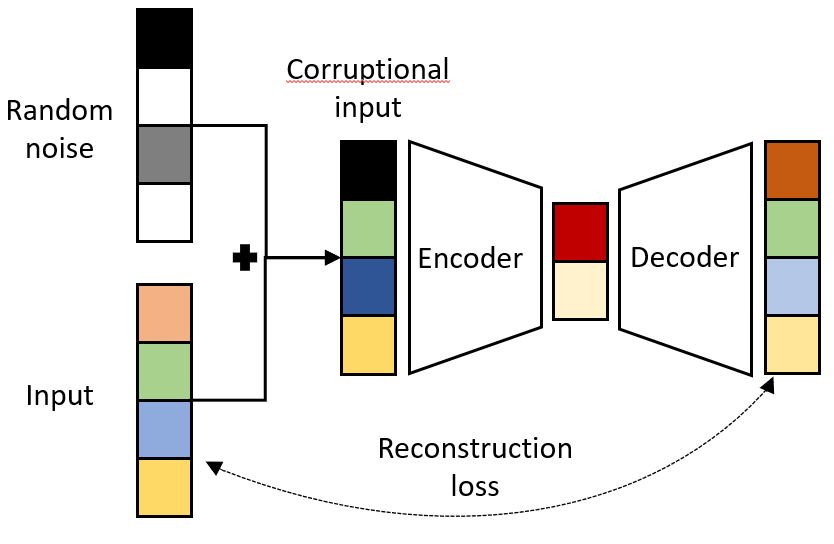
\includegraphics[width=.6\textwidth]{gfx/literature/dae}
  \caption{Der DAE minimiert den Fehler zwischen der Rekonstruktion des modifizierten Eingabevektors und der Eingabe. Abbildung entnommen aus \cite{LopezPinaya2019}}
\end{figure}

Abb. \ref{fig:ae_reconstruction} zeigt zwei Rekonstruktionen von Merkmalsvektoren. Man beachte, dass ein zufälliges Sample aus dem Merkmalsraum mehr einem Rauschen als einer tatsächlichen Klasse aus dem Datensatz ähnelt. Denn die Räume zwischen den codierten Merkmalsvektoren sind im Allgemeinen nicht definiert. Der Merkmalsraum besitzt keine "geometrische" Struktur. Um dieses Problem zu lösen wurde eine weitere Klasse von Autoencodern entworfen: Variational Autoencoder.



\section{Variational Autoencoder}\label{sec:VAE_introduction}\label{sec:variational_autoencoder}
\cite{Kingma2014} betrachten in ihrer Arbeit das Konzept des Autoencoders aus einer probabilistischen Sicht. Der Encoder bildet die Eingabe nicht auf einen eindeutigen Merkmalsvektor, sondern auf eine Wahrscheinlichkeitsverteilung über den Merkmalsraum ab. Damit bekommt der Merkmalsraum eine probabilistische Struktur. Die Herleitung des Variational Autoencoders erfolgt üblicherweise über das Konzept von latenten Variablen, welches im Folgenden näher erläutert wird. Die Herleitung Orientiert sich an den Arbeiten von \cite{Kingma2014} und \cite{Doersch2016}.


\subsection{Latente Variablen}
Latente Variablen sind nicht beobachtbare Zufallsvariablen (ZV), welche aber aus einem mathematischen Model heraus gefolgert werden können. Eine Latente Variable kann zum Beispiel eine codierte Merkmalsbeschreibung eines Bildobjektes sein. Diese gibt vor wie das Objekt aussieht, tatsächlich beobachtet werden, kann aber nur das Objekt selbst. Den Zufallsraum der latenten Variable wird Latent-Space genannt.\\
In den anschließenden Kapiteln werden die folgenden Bezeichnungen verwendet:
\begin{itemize}
  \item $\cD$, der Datensatz über einen Raum $\cX$, respektive $x \sim D$, mit $x \in X$ ein beliebiger Datenpunkt aus dem Datensatz.
  \item $\cZ = \bR^d$, der Latent-Space mit Dimension $d$
  \item $P\left[ \cZ\right]$ eine "probability density function" (PDF) über $\cZ$.
  \item $\mu_\phi: \cX \rightarrow \cZ$, eine beliebige Funktion parametrisiert durch $\phi$. Wird im folgenden verwendet, um den Erwartungswert einer Normalverteilung $\cN$ zu approximieren.
  \item $\sigma_\phi: \cX \rightarrow \cZ$, analog zu $\mu_\phi$, die Varianz der Normalverteilung $\cN$.
  \item $g_\theta: \cZ \rightarrow \cX$, beliebige Funktion parametrisiert durch $\Theta$. Repräsentiert den Decoder.
\end{itemize}
$\mu_\phi(x)$ und $\sigma_\phi(x)$ repräsentieren gemeinsam die Ausgabe des Encoders für Eingabe $x$.\\

Sei die PDF $P\left[ \cZ \right]$ beliebig aber fest. Außerdem sei $z \in Z$ eine Latente Variable, mit $z \sim P\left[ \cZ\right]$. Für ausreichend komplexe $g_\theta$ kann durch die Wahl von $\Theta$ jede beliebige Verteilung mittels $g_\theta$ modelliert werden (Inverse-Transform-Sampling). Sei nun $P_\theta(x \vert z) = P\left(g_\theta(z) = x \right)$ die bedingte Wahrscheinlichkeit des Auftretens von $x$. Über Marginalisierung erhalten wir:
\begin{equation}\label{eq:max_likelihood}
  P_\theta(x) = \bE_{z \sim P(\cZ)} \left[ P(x \vert z) \right] = \int_{\cZ} P_\theta(x \vert z) \cdot P(z) dz
\end{equation}
Um den Datensatz möglichst gut zu repräsentieren, soll $P_\theta\left[ \cX \right]$ nach der "Maximum-Likelihood" Methode maximiert werden. Dazu sind folgende Ableitungen nötig:
\begin{equation}
  \frac{\partial}{\partial \theta} P_\theta(x) = \int_{\cZ} \frac{\partial}{\partial \theta}P_\theta(x \vert z) \cdot P(z) dz
\end{equation}
Dieses Integral ist im Allgemeinen nicht lösbar. Dennoch kann es approximiert werden. Eine Möglichkeit dies zu tun ist Monte-Carlo-Integration. Dieser Ansatz ist allerdings nicht effizient, denn $\cZ$ ist überabzählbar. Erweiterungen der Monte-Carlo Integration (z.B. "Importance Sampling") sind auch nicht anwendbar, da keine Annahmen über die Verteilung $P_\theta(x \vert z)$ möglich sind. Bekannt ist aber, dass $P_\theta(z \vert x)$ die bedingte Wahrscheinlichkeit darstellt, dass $z$ im Urbild (bzgl. $g_\phi$) von $x$ liegt, sprich $z$ ist Erzeuger von $x$. Ziel ist es, $P_\theta(z \vert x)$ zu approximieren, um gezielt die $z$ zu sampeln, welche $x$ erzeugen. Gesucht ist also eine Verteilung $Q\left[ \cZ \right]$, welche ähnlich zu $P_\theta\left[ \cZ \vert x\right]$ ist. Dazu wird im anschließenden Abschnitt die Kullback-Leibler Divergenz eingeführt.


\subsection{Kullback-Leibler Divergenz}
Die Kullback-Leibler Divergenz, kurz KL Divergenz oder $\cD_{KL}$, ist ein Maß für die Ähnlichkeit zweier Wahrscheinlichkeitsverteilungen. Für beliebige Verteilungen $Q, P$ über eine Menge $\cX$ ist sie definiert als:
\begin{equation}
  \cD_{KL}\left[ Q \| P\right] = \bE_{x \sim Q}\left[ \log Q(x) - \log P(x)\right]
\end{equation}
Mit der KL Divergenz und dem Satz von Bayes kann die Beziehung zwischen $P(x)$ und $\bE_{z \sim Q}\left[ P(x \vert z )\right]$ formuliert werden:
\begin{align}
  \cD_{KL}\left[ Q\left[ \cZ \right] \| P_\theta\left[ \cZ \vert x\right] \right] &= \bE_{z \sim Q}\left[ \log Q(z) - \log P_\theta(z \vert x)\right] \\
  &= \bE_{z \sim Q}\left[ \log Q(z) - \log(\frac{P_\theta(x \vert z) \cdot P(z)}{P_\theta(x)})\right] \notag\\
  &= \bE_{z \sim Q}\left[ \log Q(z) - \log P_\theta(x \vert z) - \log P_\theta(z) + \log P_\theta(x)\right] \notag
\end{align}
Da $\log P_\theta(x)$ nicht von $z$ abhängt kann dieser Term aus dem Erwartungswert gezogen werden.
\begin{equation}
  \cD_{KL}\left[ Q(z) \| P_\theta(z \vert x)\right] = \bE_{z \sim Q}\left[ \log Q(z) - \log P_\theta(x \vert z) - \log P(z)\right] + \log P_\theta(x) \notag
\end{equation}
Dies ist äquivalent zu:
\begin{align}
  \underbrace{\log P_\theta(x)}_\text{Log-Likelihood} - \underbrace{\cD_{KL}\left[ Q\left[ \cZ \right] \| P_\theta\left[ \cZ \vert x\right] \right]}_\text{Error Term} &= - \bE_{z \sim Q}\left[ \log Q(z) - \log P_\theta(x \vert z) - \log P(z)\right] \notag\\
  &= \bE_{z \sim Q}\left[ \log(P_\theta(x \vert z)\right] - \cD_{KL}\left[ Q(z) \| P(z)\right] \label{eq:pre_objective}
\end{align}
Zu sehen ist auf der linken Seite dieser Gleichung zunächst die logarithmierte Wahrscheinlichkeit von $x$ (Log-Likelihood), welche maximiert werden soll. Von dieser wird die KL-Divergenz von $Q$ und $P$ subtrahiert. D.h. $P_\theta(x)$ wird maximiert und gleichzeitig $Q\left[ \cZ \right]$ dafür bestraft, zu weit von der tatsächlich unterliegenden Verteilung $P_\theta\left[ \cZ \vert x\right]$ abzuweichen. Die rechte Seite besteht aus dem Erwartungswert von $z \sim Q$ über folgende Terme: Die Log-likelihood $g_\phi(z) = x$ und die KL-Divergenz von $Q(z)$ und $P(z)$. Man beachte, dass $g_\phi(z)$ berechnet werden kann und $P\left[ \cZ \right]$ beliebig ist. Es wird nun $P\left[ \cZ \right]$ und $Q$ spezifiziert. Üblicherweise wird $P\left[ \cZ \right]$ als $\cN(0, I)$ gewählt ($I \in \bR^{d \times d}$ ist die Einheitsmatrix) . $Q\left[ \cZ \right]$ wird parametrisiert durch $Q_\phi\left[ \cZ \vert x \right] = \cN(\mu_\phi(x), \sigma_\phi(x))$. $\sigma_\phi(x)$ ist die Hauptdiagonale der Kovarianzmatrix $\Sigma_\phi(x)$. Eine Annahme für VAEs ist nähmlich, dass die Dimensionen in $\cZ$ unkorreliert sind und folglich $\Sigma_\phi$ diagonal ist. Vorteil dieser Parametrisierung von $Q$ ist, dass sich die Ableitung der KL-Divergenz von Normalverteilungen effizient berechnen lässt. Einsetzen in \ref{eq:pre_objective} ergibt:
\begin{align}\label{eq:objective}
  &\log P_\theta(x) - \cD_{KL}\left[ Q\left[ \cZ \right] \| P_\theta\left[ \cZ \vert x\right] \right] \notag\\[8pt]
  =& \, \bE_{z \sim \cN(\mu_\phi(x), \sigma_\phi(x))}\left[ \log \underbrace{P_\theta(x \vert z)}_\text{Decoder} - \cD_{KL}[\underbrace{\cN(\mu_\phi(x), \sigma_\phi(x))}_\text{Encoder} \| \cN(0, I)] \right]
\end{align}
Gleichung \ref{eq:objective} zeigt direkt die Encoder-Decoder Struktur der VAE Zielfunktion.
\begin{figure}[hbt]
  \centering
  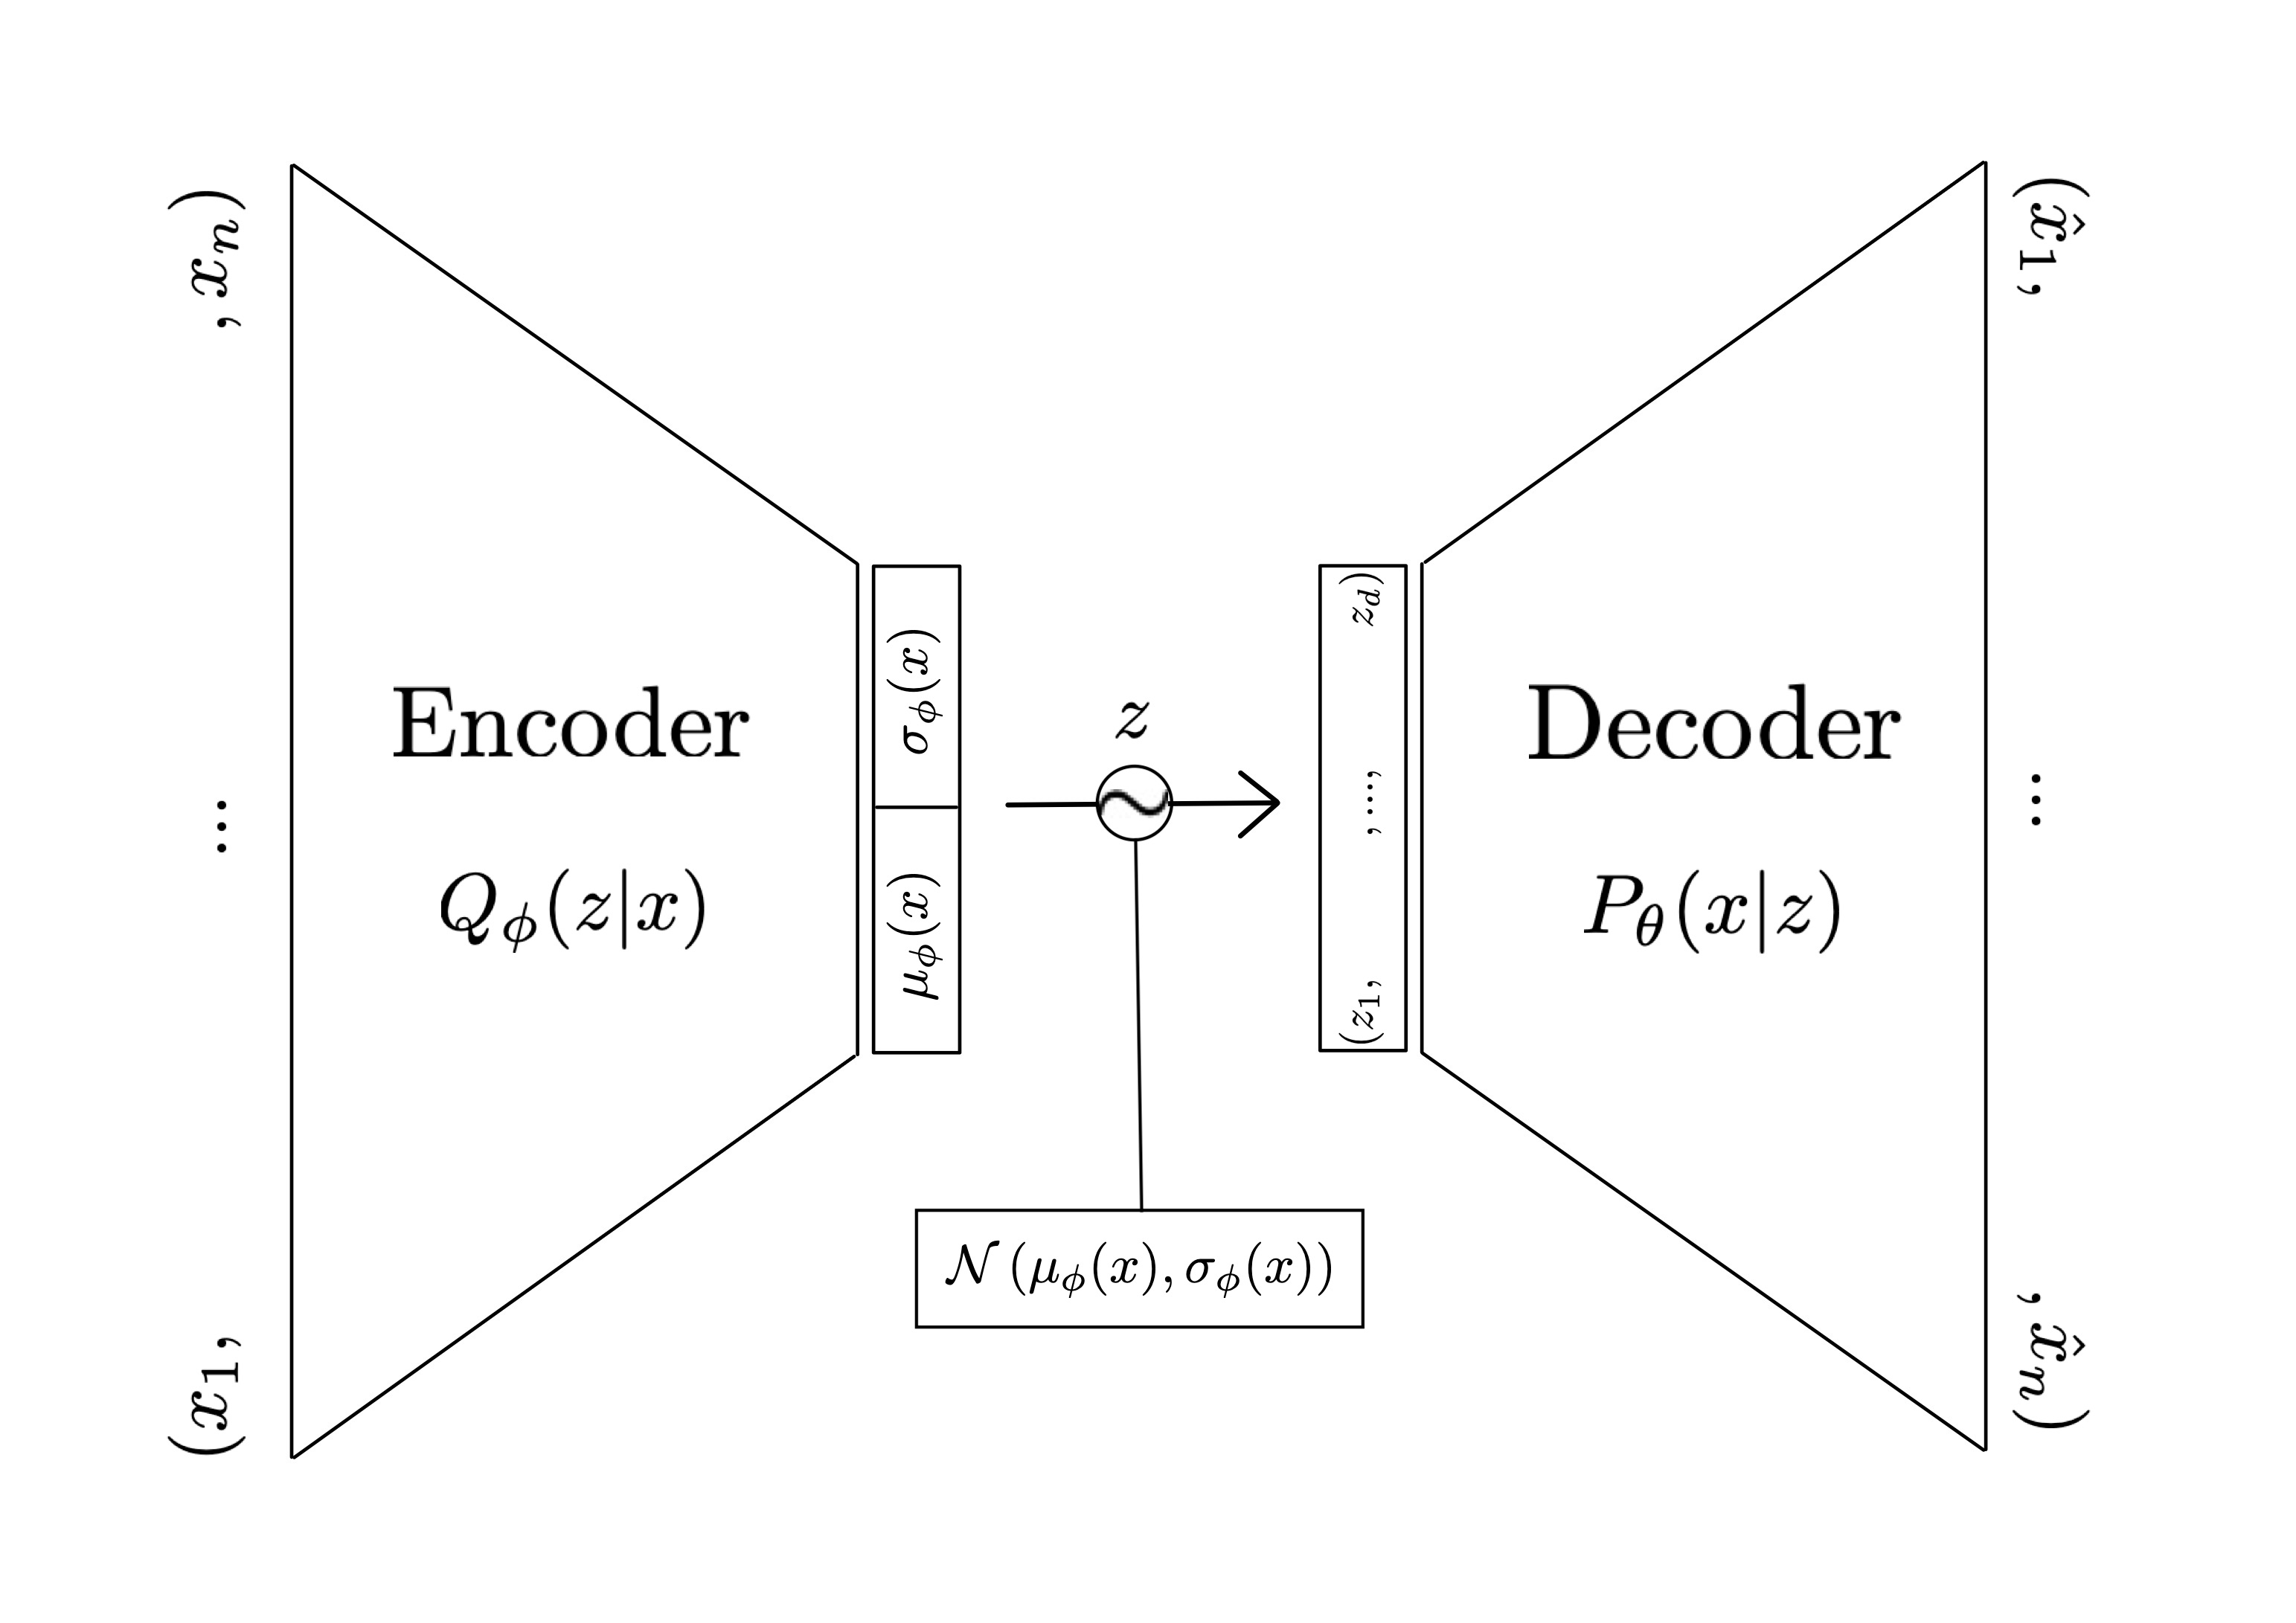
\includegraphics[width=.7\textwidth]{gfx/literature/forward_pass}
  \caption{Der Vorwärtsdurchlauf beim VAE. Der Encoder die Verteilung $Q_\phi(z \vert x)$ parametrisiert durch $\mu_\phi$ und $\sigma_\phi$. Aus dieser wird $z$ erzeugt. Anschließend liefert der Decoder die Rekonstruktionsverteilung $P_\theta(x \vert z)$ bzw. für festes $x$ die Rekonstruktion $\hat{x}$. (siehe auch \cite{Doersch2016}}
  \label{fig:enc-dec}
\end{figure}


\subsection{Optimierung der VAE Zielfunktion}\label{sec:vae_loss_func}
Statt die obige Zielfunktion zu maximieren, wird folgende Fehlerfunktion minimiert (der Einfachheit wegen wird $\mu_\phi$ statt $\mu_\phi(x)$ etc. geschrieben):
\begin{align}\label{eq:gradient}
  &\cL = - \left( \bE_{z \sim \cN(\mu_\phi, \sigma_\phi)}\left[ \log(P_\theta(x \vert z) - \cD_{KL}[\cN(\mu_\phi, \sigma_\phi) \| \cN(0, I)] \right] \right) \\
=& \, -\bE_{z \sim \cN(\mu_\phi, \sigma_\phi)}\left[ \log(P_\theta(x \vert z) \right] + \bE_{z \sim \cN(\mu_\phi, \sigma_\phi)}\left[ \cD_{KL}[\cN(\mu_\phi, \sigma_\phi) \| \cN(0, I)] \right]
\end{align}
Der erste Term entspricht dem komponentenweisen "Negative-Log-Likelihood" (NLL) Fehler der Eingabe $x$ und der Rekonstruktion $g_\theta(z)$. $z$ wird aus der Encoder Verteilung $\cN(\mu_\phi, \sigma_\phi)$ gesampelt. Für die KL Divergenz zweier Normalverteilungen existiert eine geschlossene Form zur Berechnung (siehe \cite{kl_divergence_close_form}):
\begin{align}
  &\cD_{KL}\left[ \cN(\mu_0, \Sigma_0) \| \cN(\mu_1, \Sigma_1)\right] = \notag\\
  &\frac{1}{2}\left( \Spur(\Sigma_1^{-1}\Sigma_0) + (\mu_1 - \mu_0)^T\Sigma_1^{-1}(\mu_1 - \mu_0) - k + \log(\frac{\det\Sigma_1}{\det\Sigma_0})\right)
\end{align}
Durch Einsetzen von $\cN(\mu_\phi, \sigma_\phi)$ und $\cN(0, I)$ vereinfacht sich die Gleichung zu:
\begin{align}
  &\cD_{KL}\left[ \cN(\mu_\phi, \Sigma_\phi) \| \cN(0, I)\right] = \notag\\
  &= \frac{1}{2}\left( \sum_{i=1}^k (\sigma_\phi)_i + \sum_{i=1}^k (\mu_\phi)_i^2 - \sum_{i=1}^k 1 - \log(\prod_{i=1}^k (\sigma_\phi)_i)) \right) \notag\\
  &= \frac{1}{2} \sum_{i=1}^k\left((\sigma_\phi)_i + (\mu_\phi)_i^2 - 1 - \log (\sigma_\phi)_i \right)
\end{align}
Die Ableitung des KL-Terms ist somit berechenbar. Für die Ableitung des NLL Fehlers nach dem Parametern $\phi$ des Encoders besteht jedoch folgendes Problem:
\begin{equation}
  \frac{\partial}{\partial \phi} (- \bE_{z \sim \cN(\mu_\phi, \sigma_\phi)}\left[ \log g_\theta(z) \right] )
\end{equation}
Da $z$ aus einer Zufallsverteilung gesampelt wird, kann keine Ableitung nach $\phi$ gebildet werden. Als Lösung wird der folgende Trick angewandt.

\subsection{Reparametrisierungs-Trick}\label{sec:reparam_trick}
Eine Ableitung des NLL Fehlers ist nach den Parametern $\phi$ des Encoder Netzwerks wegen des Samplings von $z \sim \cN(\mu_\phi, \sigma_\phi)$ nicht möglich. Statt aber direkt aus der Verteilung zu sampeln, kann ein $\epsilon \sim \cN(0, I)$ gesampelt werden und die gleiche Verteilung durch Multiplikation und Addition berechnet werden. Für $z \sim \cN(\mu_\phi(x), \sigma_\phi(x))$ gilt also:
\begin{equation}
  z = (\sigma_\phi(x))^{\frac{1}{2}} \cdot \epsilon + \mu_\phi(x)
\end{equation}
D.h. von folgender Gleichung kann die Ableitung nach $\phi$ berechnet werden:
\begin{equation}
  \frac{\partial}{\partial \phi} \left(- \bE_{x \sim D}\left[ -\bE_{\epsilon \sim \cN(0, I)}\left[ \log g_\theta\left(z = (\sigma_\phi(x))^{\frac{1}{2}} \cdot \epsilon + \mu_\phi(x)\right)\right] \right] \right)
\end{equation}

	
	% Datasets
	\chapter{Datensätze}\label{cpt:datasets}
Diese Arbeit wie bereits in der Einführung erläutert, ist ein Aspekt dieser Arbeit den VAE basierten Data Augmentation Ansatz auf unterschiedlichen Daten zu evaluierten. Dazu werden sowohl Bilddaten, als auch numerische Daten evaluiert. Zusätzlich wird die Datensatzgröße variiert. Im folgenden werden die verwendeten Datensätze und ihre Besonderheiten näher beschrieben.



\section{MNIST}\label{sec:MNIST}
\begin{figure}[hbt]
  \centering
  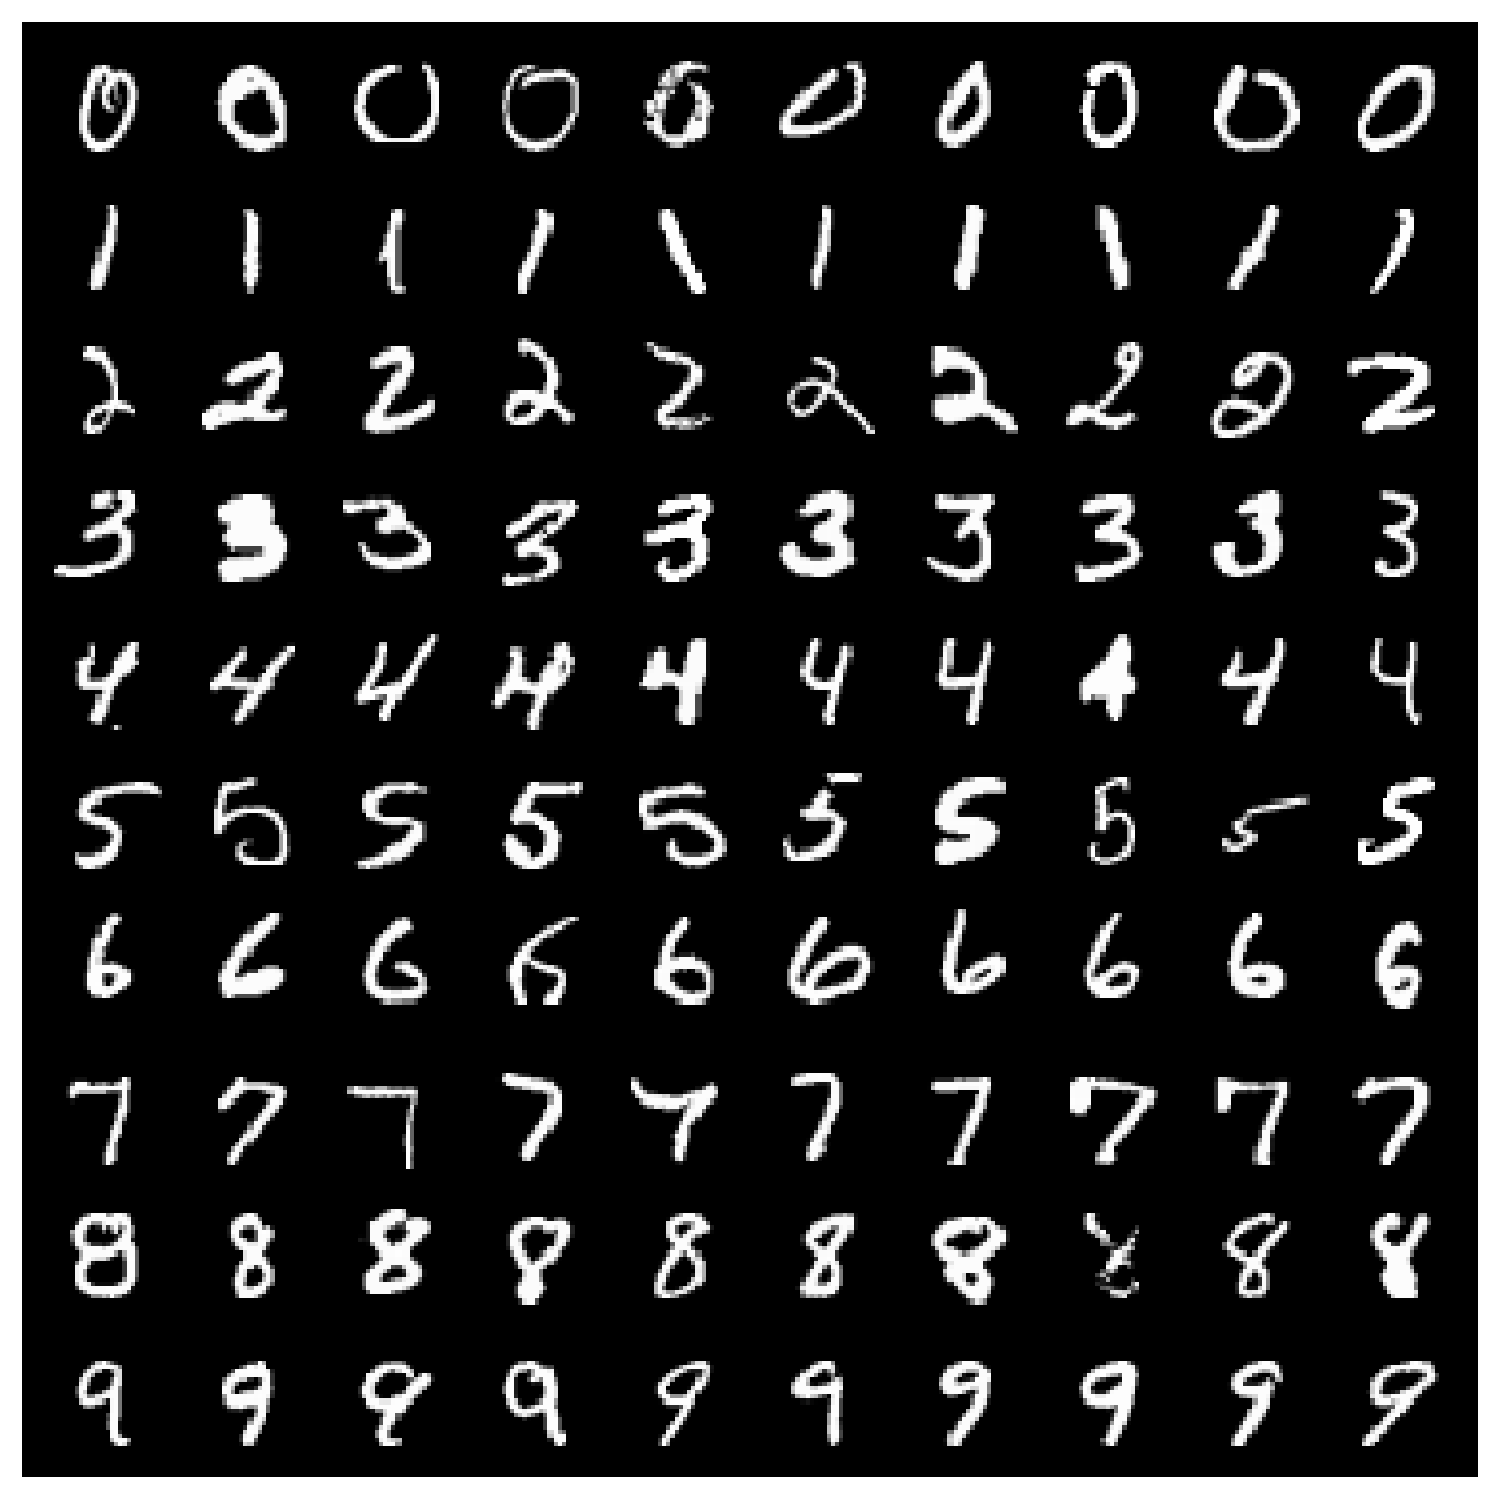
\includegraphics[width=.4\textwidth]{gfx/datasets/mnist_ciffers}
  \caption{Der MNIST Datensatz beinhaltet annotierte Bilder der handgeschriebenen Zahlen $\lbrace0, \dots, 9\rbrace$}
\end{figure}
Der MNIST Datensatz von \cite{lecun-98} wird oft verwendet, um neue Ansätze im Bereich Visual Machine Learning auf ihre Nutzbarkeit hin zu untersuchen. Es handelt sich bei den Daten um $(28 \times 28)$ Pixel große Grauwertbilder handgeschriebener Zahlen $\lbrace0, \dots, 9\rbrace$. Es gibt zwei Partitionen des Datensatzes: Die Trainings-Partition besteht aus 60.000 Beispielen, also 6.000 pro Klasse. Die Test-Partition beinhaltet 10.000 Beispiele. Die Klassifikation von MNIST ist über die letzten Jahre nahezu fehlerfrei gelöst (z.B. von \cite{byerly2021branching}), da die Daten klar voneinander unterscheidbar sind, der Datensatz balanciert ist und ausreichend Beispiele besitzt. \\

Da die MNIST Aufgabe wegen der genannten Eigenschaften schon durch einfache Modelle gut gelöst werden kann, werden in dieser Arbeit ausschließlich reduzierte Versionen des Originaldatensatzes betrachtet. Die Reduktion erfolgt durch zufälliges Wählen von Beispielen aus der Trainings-Partition des Datensatzes. Für die Evaluation wird der unveränderte Test-Teil verwendet.



\section{PROBEN1}\label{sec:PROBEN1_dataset}
PROBEN1 ist eine Zusammenfassung mehrerer Datensätze, welche verschiedenste Diagnoseinformationen (Attribute) enthalten, die eine Klassifikation ermöglichen. Vorgeschlagen wurde dieser Datensatz von \cite{Moreno-Barea2020} um verschiedene Generative Modelle auf kleinen teilweise imbalancierten Datensätzen zu evaluieren. Es ist ein rein numerischer Datensatz, bei dem jede Dimension des Eingabevektors ein Attribut (z.b. Alter, BMI, etc.) beschreibt. Nicht alle diese Attribute entsprechen kontinuierlichen Werten, daher wurden alle Daten, kontinuierliche und diskrete, normalisiert. Fehlende Daten (im Original durch ein "?" repräsentiert) wurden durch Nullen ersetzt. Im Gegensatz zu MNIST und anderen Bild-Datensätzen spielt die relative Position der Attribute im Eingabevektor keine Rolle. Dies wird bei der Wahl der Modellarchitektur für diesen Datensatz berücksichtigt.
 Tabelle \ref{tab:PROBEN1-datasets} gibt einen Überblick über die Dimension der Eingabevektoren (\# Attribute), die Anzahl an Klassen und die Größe und Balance der einzelnen Datensätze.
\begin{table}[hbt]
\centering
\begin{tabular}{l|l|l|l|l|l}
\toprule
Datensatz   & \# Attribute & kontinuierlich        & \# Klassen & \# Beispiele & Balancing \\ \hline
card        & 15           & 0.40                  & 2          & 690          & 0.99      \\
diabetes    & 8            & 1.00                  & 2          & 768          & 0.93      \\
geneN       & 60           & 0.00                  & 3          & 3175         & 0.93      \\
glass       & 9            & 1.00                  & 6          & 214          & 0.84      \\
horse-colic & 20           & 0.70                  & 3          & 364          & 0.84      \\
thyroid     & 21           & 0.29                  & 3          & 7200         & 0.28      \\
\bottomrule
\end{tabular}
\caption{PROBEN1 Datensatz Infos.}
\label{tab:PROBEN1-datasets}
\end{table}
Für diese Arbeit wurde jeder Datensatz in Trainings und Test-Partition aufgeteilt, wobei 80\% für das Training und 20\% für die Evaluation verwendet wurden. Zusätzlich werden reduzierte Trainings-Partitionen, analog zum Abschnitt \ref{sec:MNIST} betrachtet.


\section{CIFAR-10}
\begin{figure}[hbt]
  \centering
  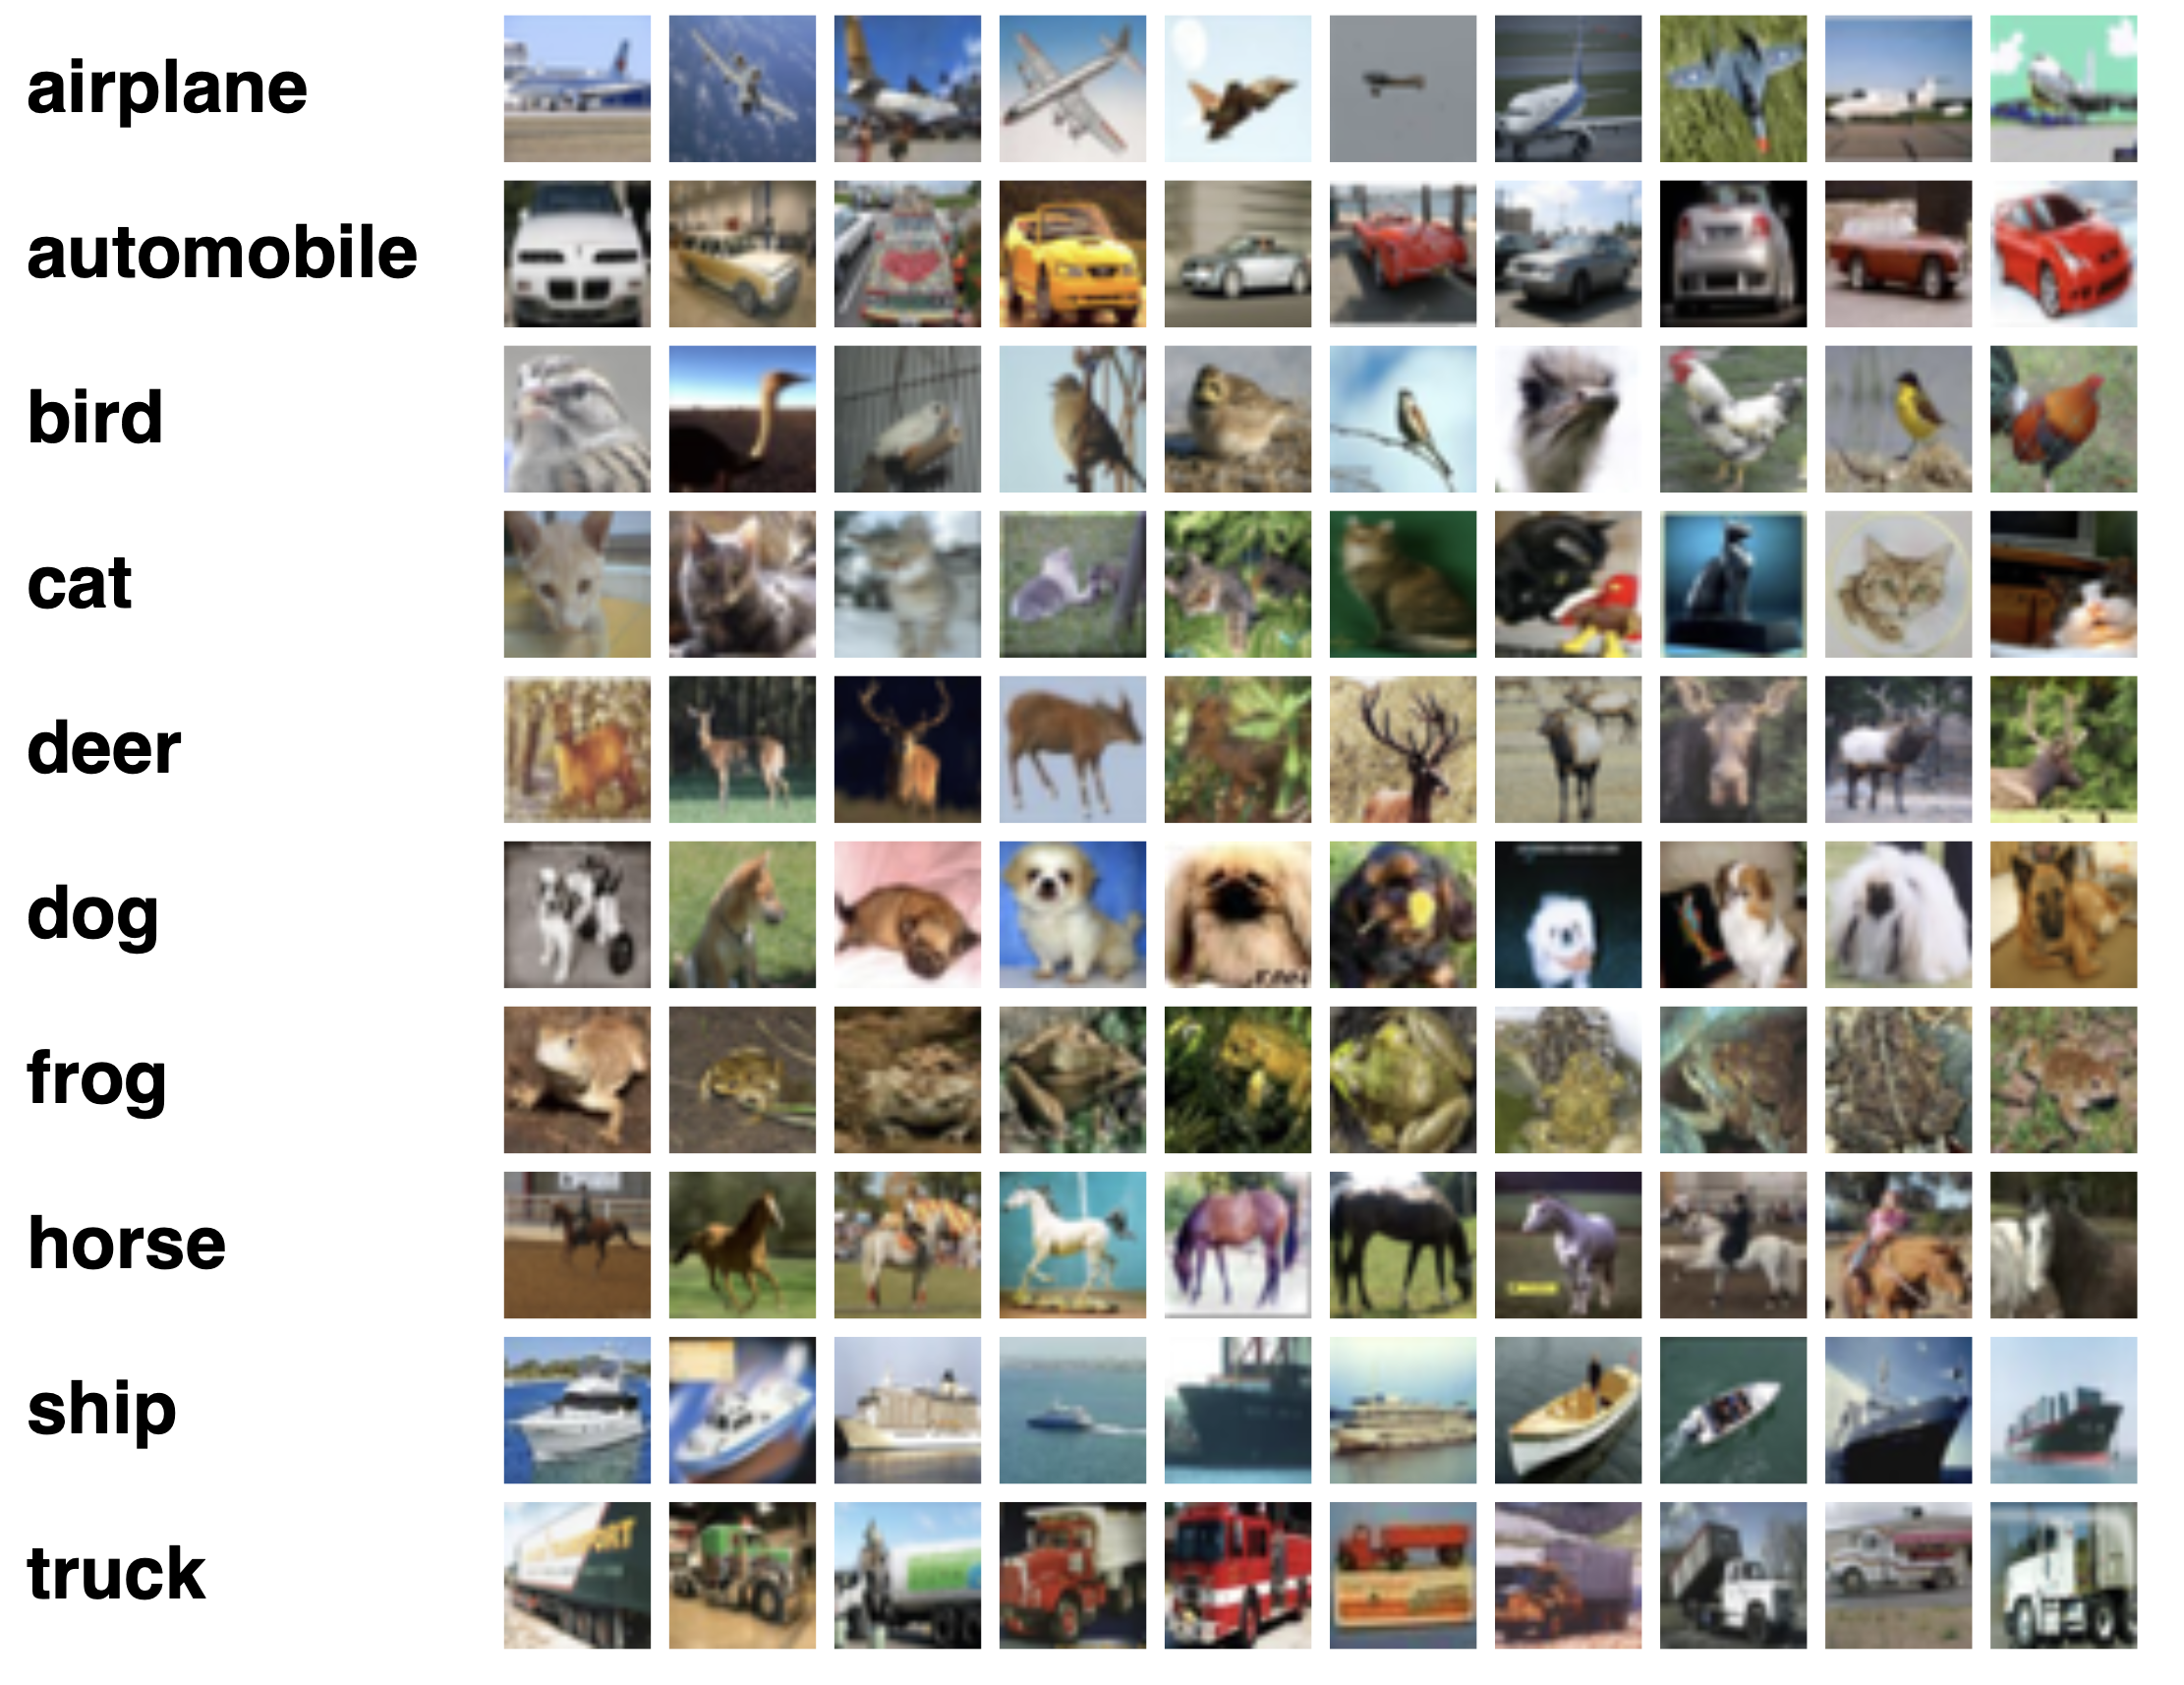
\includegraphics[width=.55\textwidth]{gfx/datasets/cifar10_dataset}
  \caption{CIFAR-10 Datensatz: Die einzelnen Klassen schließen sich gegenseitig aus, d.h. es gib z.b. keine Mischform aus "truck" und "automobile" wie SUV.}
  \label{fig:CIFAR_10_dataset}
\end{figure}
CIFAR-10 erstellt von \cite{cifar-orig} ist eine annotierte Teilmenge des "80 million tiny images" Datensatzes. Der Datensatz ist analog zu MNIST (vgl. Abschnitt \ref{sec:MNIST}) aufgeteilt in 60.000 Trainingsbeispiele und 10.000 Testbeispiele. Er enthält 10 verschiedene Klassen (siehe Abb. \ref{fig:CIFAR_10_dataset}). CIFAR-10 stellt als Klassifikationsaufgabe, wie MNIST, keine große Herausforderung da (siehe \cite{foret2021sharpnessaware}). Daher fokussiert sich diese Arbeit vor allem auf die Qualität der Rekonstruktionen auf diesem Datensatz.



\section{Large-scale CelebFaces Attributes}
\begin{figure}[hbt]
  \centering
  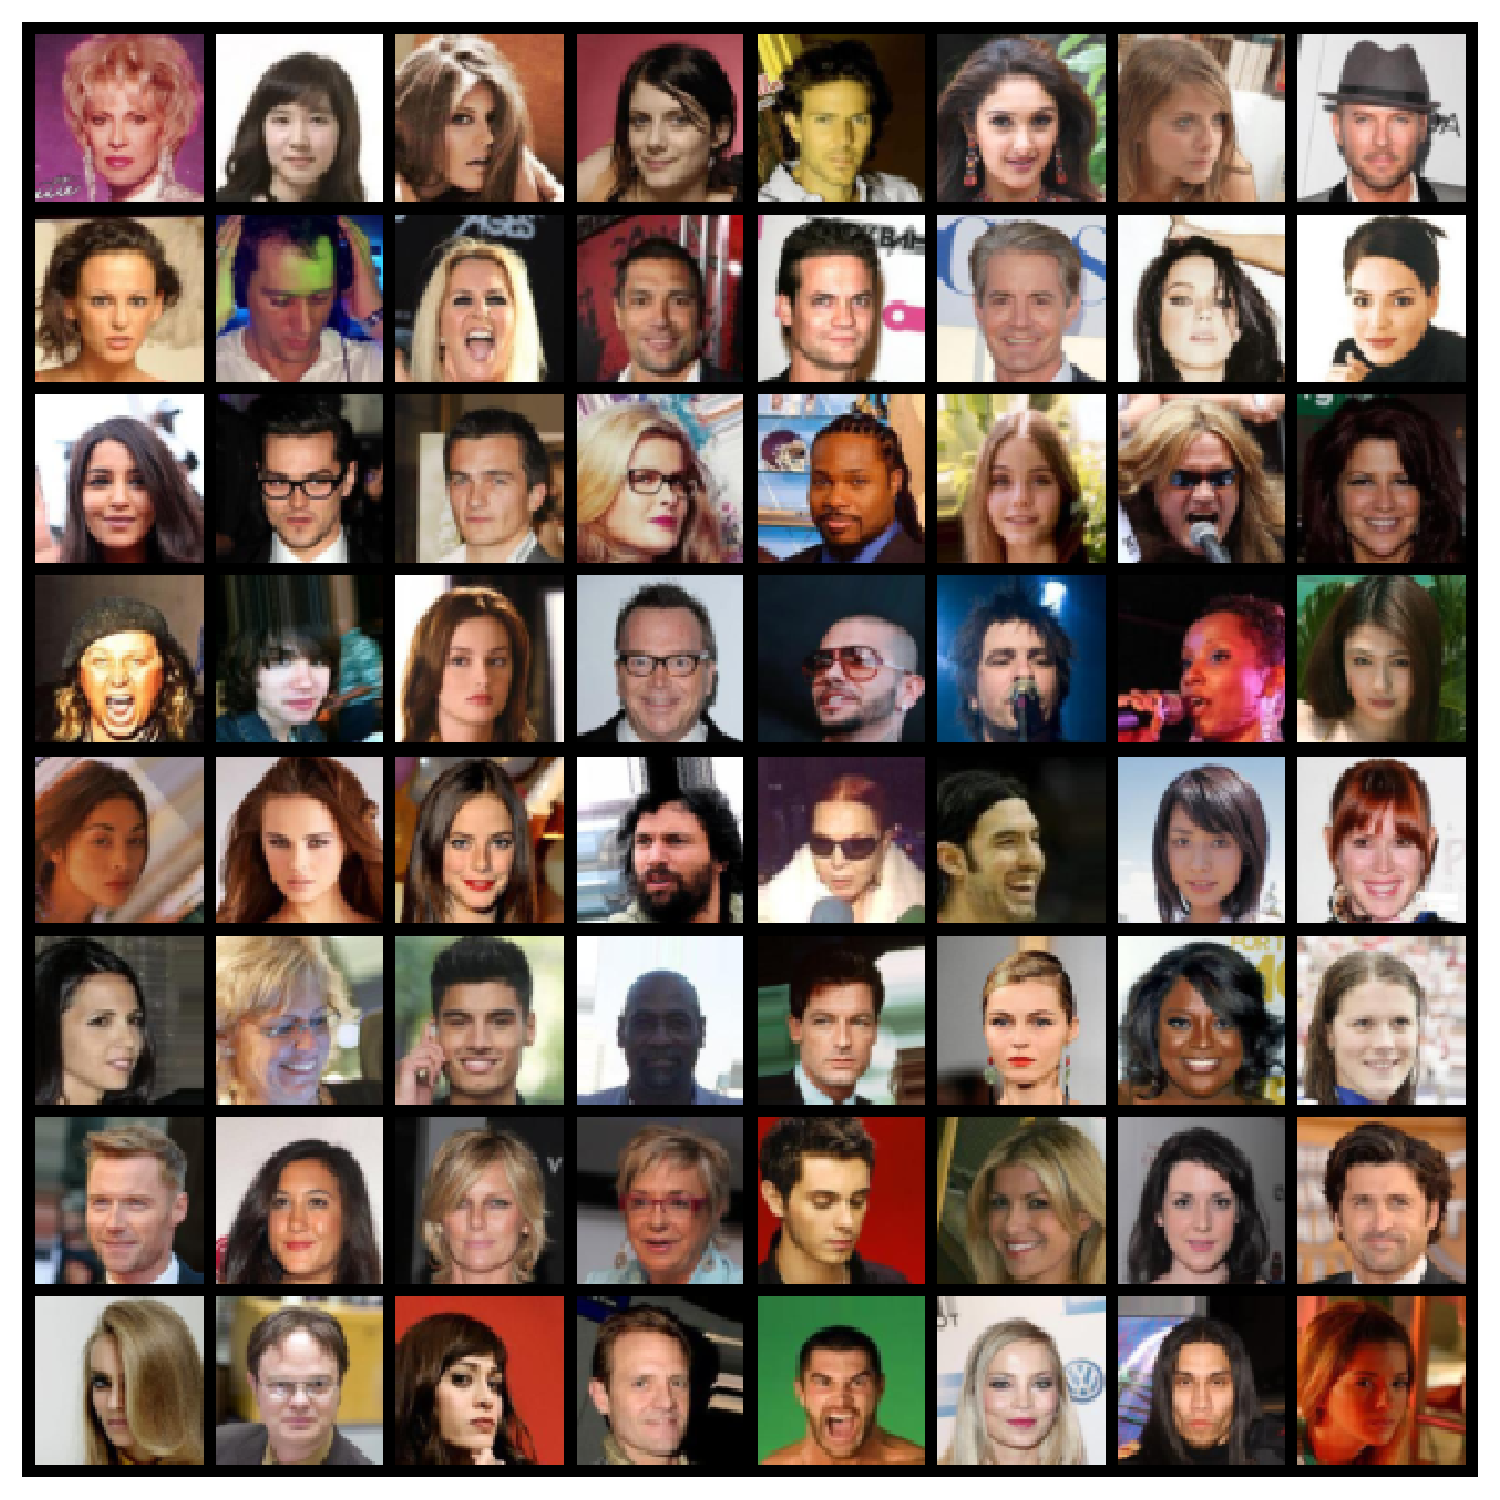
\includegraphics[width=.4\textwidth]{gfx/datasets/real}
  \caption{Die Gesichtsdaten des CelebA Datensatzes}
\end{figure}

Large-scale CelebFaces Attributes (CelebA), von \cite{liu2015faceattributes}, ist eine Sammlung von über 200.000 Bildern von Gesichten. Es gibt 10.177 verschiedene Identitäten. Jedes Bild ist mit 40 Attributen wie Haarfarbe, Brille, etc. annotiert. In dieser Arbeit wird insbesondere untersucht, wie sich Manipulationen im Merkmalsraum auf die decodierten Bilder auswirken. Da CelebA ein Multi-Label Datensatz ist (d.h. Attribute schließen sich gegenseitig nicht aus), liegt der Fokus auf der Trennung dieser Attribute im Latent-Space.

	
	% Methodology
	\chapter{Methodik}
Im Abschnitt \ref{sec:variational_autoencoder} wurde bereits die Funktionsweise und das Optimieren des VAE Modells beschrieben. Im folgenden wird erklärt, wie neue Beispiele generiert werden. Außerdem werden Details zu den Modellarchitekturen gezeigt.



\section{Latent-Space Sampling}\label{sec:sampling}
Der Variational Autoencoder besitzt einen strukturierten Latent-Space. Daher kann zwischen den Erwartungswerten $\mu_1 = \mu_\phi(x_1)$ und $\mu_2 = \mu_\phi(x_2)$ vom Encoder berechneten Normalverteilung interpoliert werden. Es werden im Folgenden vier verschiedene Sampling Methoden vorgestellt, um neue Latent-Vektoren $\hat{z}$ zu erzeugen. Diese wurden in leicht anderer Form von \cite{Jorge2018} vorgeschlagen. Die erste Methode ist aus der Standardnormalverteilung $\cN(0, 1)$ zu sampeln. Dies ist sinnvoll, da der Encoder durch den KL-Term dazu gezwungen ist, nicht zu sehr von $\cN(0, 1)$ abzuweichen. Eine weitere Methode ist, den Erwartungswert eines original Beispiels $\mu_\phi(x)$, welcher das Zentrum der dazugehörigen Normalverteilung repräsentiert, zu modifizieren. Betrachtet werden drei Modifikationen: Addieren von Gauss-Rauschen (Noise), Interpolation und Extrapolation. Für die Noise Variante wird zufälliges Rauschen einer Normalverteilung $\cN(0, \alpha)$ auf den Eingabe- Erwartungswert addiert.
\begin{equation}\label{eq:add_noise}
  \hat{z_i} = z_i + \epsilon, \epsilon \sim \cN(0, \alpha)
\end{equation}
Für die Wahl Interpolations Partner wird eine $k$-Nächster-Nachbar Suche im Latent-Space durchgeführt. Gesucht wird unter allen Erwartungswerten $\mu_\phi(x_i)$ für Eingaben $x_i$. $\hat{z}_i$ repräsentiert den modifizierten Latent-Vektor. Das Vorzeichen vor $\alpha$ bestimmt, ob interpoliert oder extrapoliert wird. $\alpha$ ist ein zu setzender Hyperparameter und definiert die Stärke der Inter-/Extrapolation
\begin{equation}
  \hat{z_i} = \pm \alpha \cdot \left[\mu_\phi(x_k) - \mu_\phi(x_i)\right] + \mu_\phi(x_i)
\end{equation}



\section{Single-VAE}
Dieses Verfahren trainiert ein VAE Modell auf dem gesamten Datensatz. Das Training erfolgt selbst-überwacht, d.h. es werden keine Informationen über die Klassen benötigt. Vorteil dieses Ansatzes ist, dass große Datenmengen genutzt werden können, welche nicht annotiert sein müssen. Es erschwert allerdings das Sampling neuer Beispiele, denn für einen Latent-Vektor $\hat{z}_i$ ist nicht definiert, welcher Klasse er angehört. Der Single-VAE wird deshalb nur mit den Sampling Methoden Noise, Interpolation und Extrapolation für die Data Augmentation genutzt. Das Originalbeispiel, welches für Generation modifiziert wird, definiert dabei die Klasse des generierten Beispiels. Weitere Ansätze, wie das Nutzen eines Klassifikators, welcher die Klasse zu $\hat{z}_i$ bestimmt, wurden nicht weiter verfolgt.



\section{Multi-VAE}\label{sec:multi-vae-intro}
Ein von \cite{Moreno-Barea2020} angeführtes Problem mit dem Single-VAE Ansatz besteht darin, dass ein einzelner VAE bei imbalancierten Datensätzen dazu tendiert, die größere Klasse im Latent-Space zu überrepräsentieren. Um dem entgegen zu wirken, schlagen die Autoren vor, nur einen VAE pro Klasse zu trainieren. Dazu werden die Daten in $k$ Submengen aufgeteilt, wobei $k$ die Anzahl der verschiedenen Klassen bezeichnet. Jede dieser $k$ Klassen besteht aus den der Klasse zugehörigen Daten. Außerdem wird eine Variante untersucht, bei der zusätzlich noch zufällige Beispiele der anderen Klassen mit einem Anteil von 20\% hinzugefügt werden (Bezeichnet mit "Mix Data"). Falls Klassen bestimmte Merkmale teilen, kann dies dem Encoder helfen, diese zu extrahieren. Die Abbildung \ref{fig:dataset_parts} veranschaulicht die Aufteilung des Datensatzes. Das Training der einzelnen VAEs erfolgt auf den klassenweisen Datensätzen. Neue Beispiele können somit leicht über Sampling aus einer Standard Normalverteilung generiert werden. Die Klasse des neuen Beispiels ist die zugehörige Klasse des VAEs.

\begin{figure}[hbt]
  \centering
  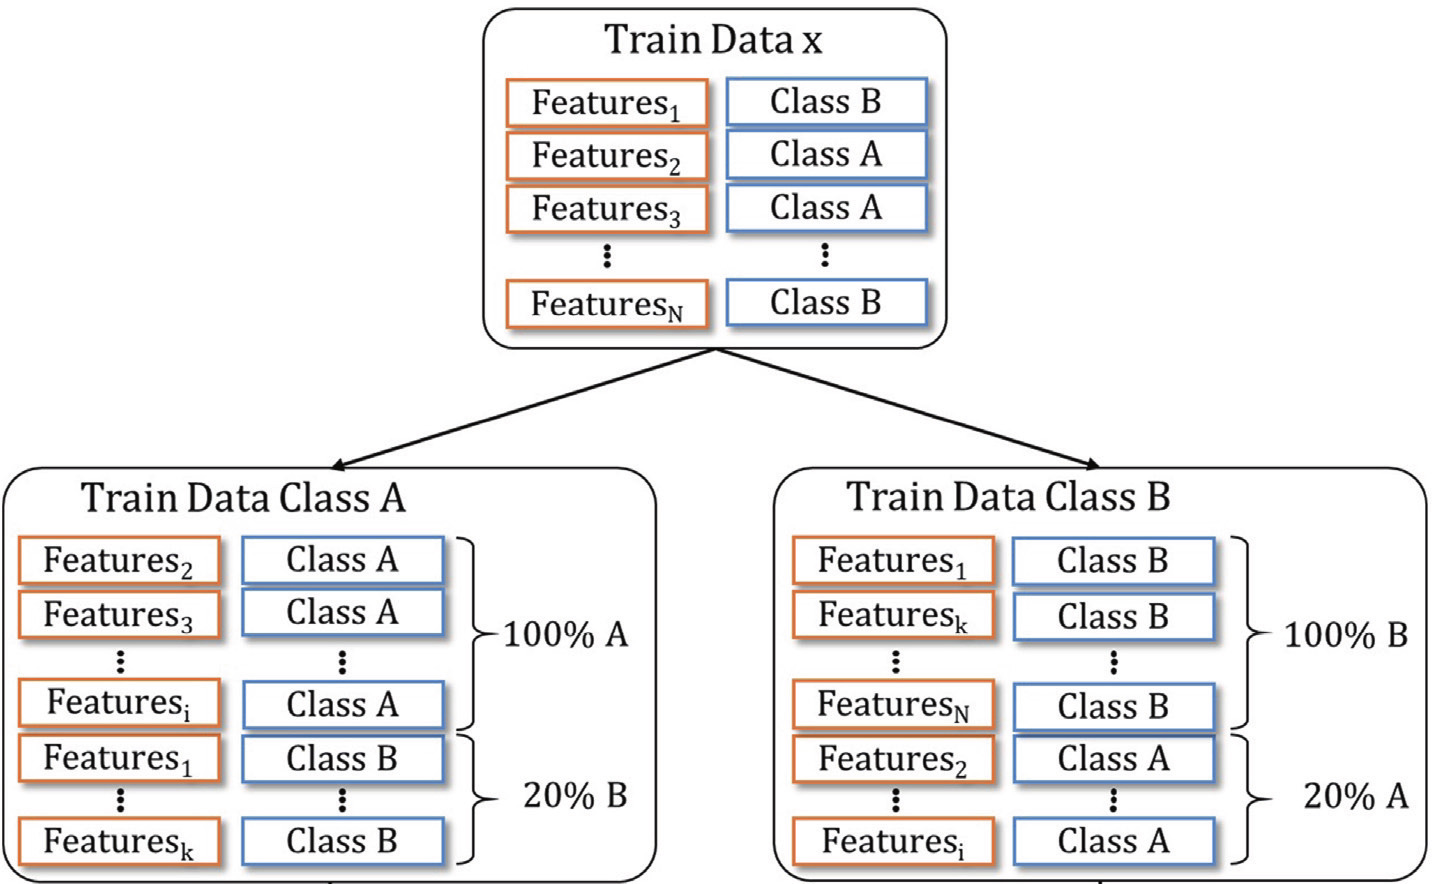
\includegraphics[width=.6\textwidth]{gfx/methodology/ds_split}
  \caption{Die Aufteilung der Datensätze beim Multi-VAE Ansatz. Der vollständige Datensatz wird in klassenweise partitioniert. Zusätzlich wird der Ansatz betrachtet, zu den Daten der Klasse $i$ auch Daten der anderen Klassen beizumischen. Bei mehr als 2 verschiedenen Klassen werden die 20\% zusammen aus zufälligen Beispielen der jeweils anderen Klassen gebildet. Abbildung entnommen aus \cite{Moreno-Barea2020}}
  \label{fig:dataset_parts}
\end{figure}



\section{Generative Classifiers}
Da der VAE darauf trainiert wird, nicht Merkmalsvektoren sondern Latent-Vektoren, welche aus einer Distribution gesampelt werden, zu decodieren, sind die generierten Beispiele häufig unscharf oder entsprechen nicht-interpretierbaren Mischformen zweier Klassen. \cite{Moreno-Barea2020} schlagen daher ein weiteres Neuronales Netz, den "Generative Classifier" (GC), vor, um diese Beispiele zu erkennen und zu verwerfen. Dazu wird zu jedem Eingabebeispiel $x$ eine verrauschte Variante $\tilde{x}$ erzeugt. Das Netzwerk wird auf die binäre Klassifikation von Rauschen und Originalbeispiel trainiert. \cite{Moreno-Barea2020} verwenden Rauschen aus zwei Quellen:
\begin{itemize}
  \item Uniformes Rauschen: Repräsentiert, dass dieses Beispiel "nur Rauschen" beinhaltet
  \item Normalverteiltes Rauschen: Repräsentiert verrauschte Originalbeispiele. Der Erwartungswert der Normalverteilung ist der Sample-Mean über die Originalbeispiele und die Varianz ist ein einstellbarer Hyperparameter $\sigma_{gc}$
\end{itemize}
Mit $\sigma_{gc}$ kann die Sensitivität des Generative Classifiers beeinflusst werden.\\

Da auf Bilddaten die verrauschten Beispiele $\tilde{x}$ nicht den verrauschten Beispielen des VAEs entsprechen, wird in dieser Arbeit eine weitere Art von Trainings Beispielen für den GC vorgeschlagen. Während des VAE Trainings wird eine frühe Version des Modells zwischengespeichert. Diese frühe Modellversion erzeugt in der Regel noch sehr verrauschte Rekonstruktionen. Diese können genutzt werden, um den GC darauf zu trainieren. Diese Art des GC wird auf dem MNIST Datensatz verwendet.

\begin{figure}[hbt]
  \centering
  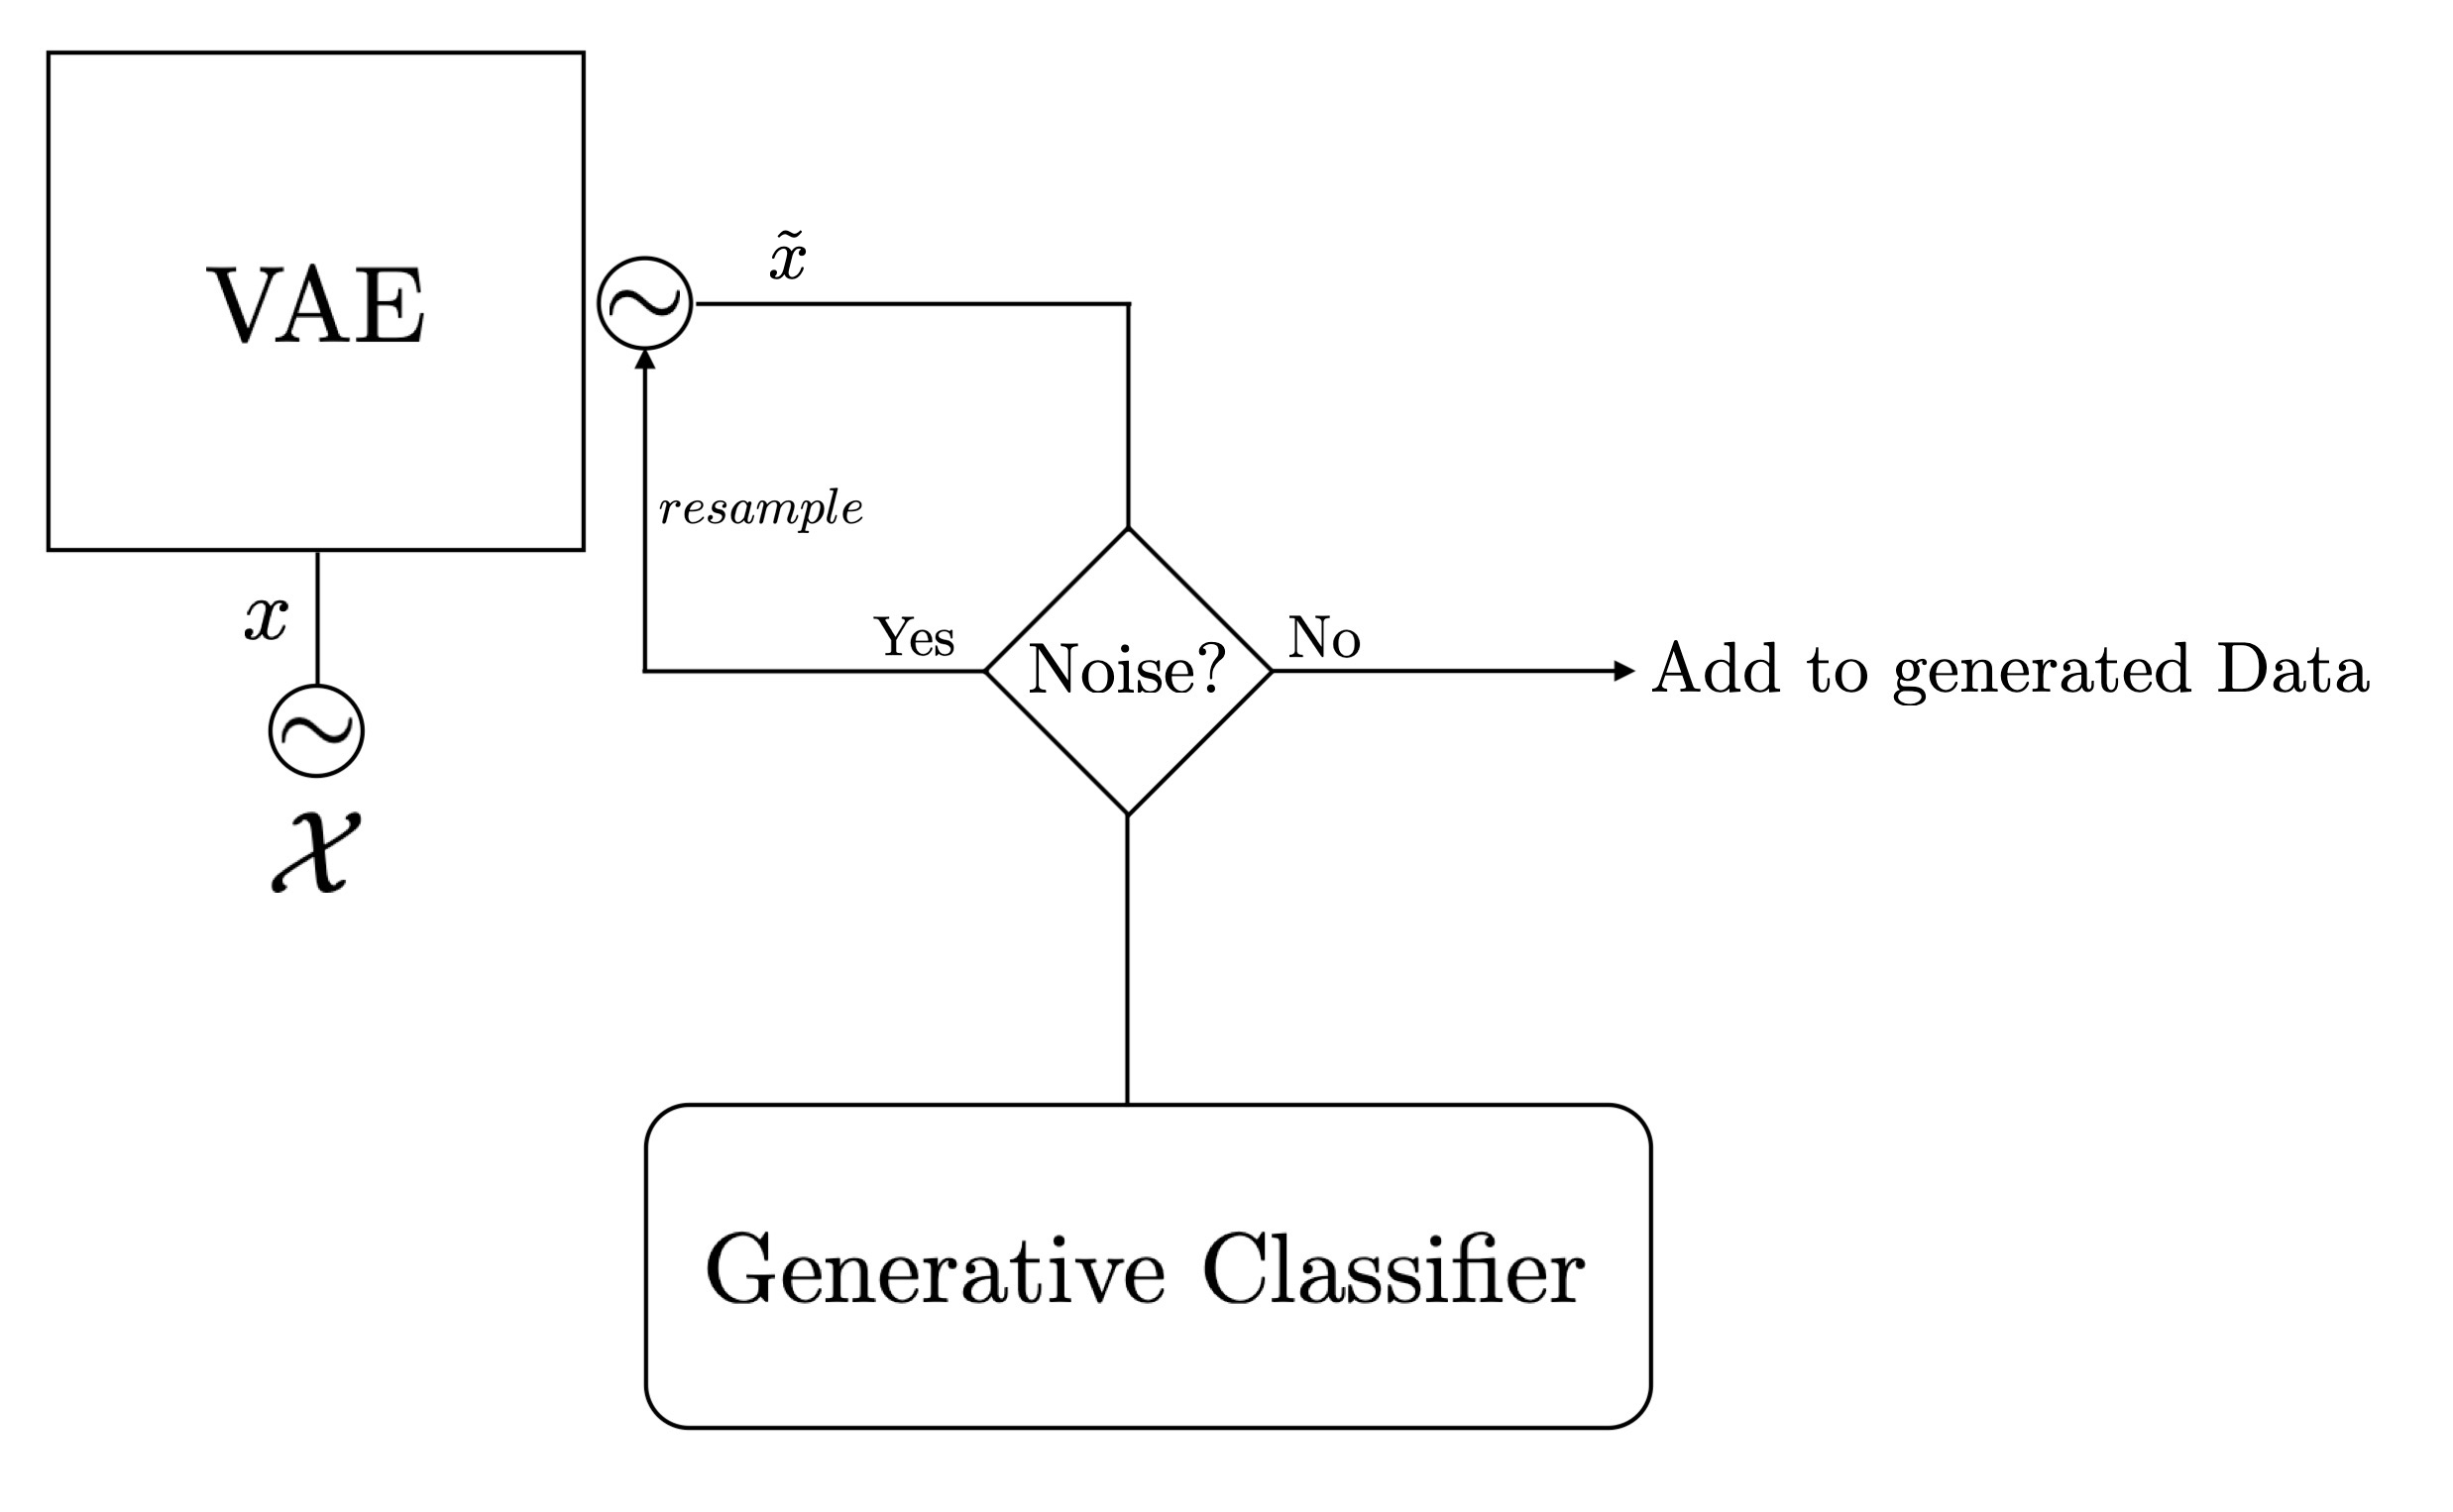
\includegraphics[width=.8\textwidth]{gfx/methodology/gc}
  \caption{Der Generative Classifier dient dazu, verrauschte und verschwommene Daten während des Generations Prozesses auszusortieren. Wenn ein generierter Datenpunkt $\tilde{x}$ als \textit{Noise} klassifiziert wird, erzeugt der VAE ein neues Beispiel.}
\end{figure}



\section{Details zu den VAE Modellarchitekturen}
Wie schon im Abschnitt \ref{sec:VAE_introduction} eingeführt besteht der Variational Autoencoder aus einem Encoder und einem Decoder Teil.
Der Encoder extrahiert Merkmale aus der Eingabe $x$ und bildet diese auf eine $d$-dimensionale Normalverteilung $Q_\phi(z \vert x) = \cN(\mu_\phi(x), \sigma_\phi(x))$ ab. Die Verteilung ist durch die Ausgaben $\mu_\phi(x)$ und $\sigma_\phi(x)$ des Encoders parametrisiert. Man beachte, dass aus numerischen Gründen tatsächlich die logarithmische Varianz $\log \sigma_\phi(x)$ berechnet wird. Das in Abschnitt \ref{sec:reparam_trick} beschriebene Sampling findet nur während des Trainings statt. Für das Generieren neuer Beispiele wurden die in \ref{sec:sampling} erklärten Sampling Methoden genutzt. Wie im Abschnitt \ref{sec:autoencoder} motiviert, wurden auf Bilddaten Konvolutionen für die Merkmalsextraktionen im Encoder verwendet. Der Decoder besteht respektive aus den entsprechenden transponierten Konvolutionen, welche den Latent-Vektor auf Bildgröße hochskalieren. Für die numerischen Daten des Datensatzes PROBEN1 werden keine Konvolutionen verwendet, da die Eingabeattribute dieses Datensatzes eindimensional und unabhängig voneinander sind (vgl. Abschnitt \ref{sec:PROBEN1_dataset}).

Für unsere Experimente wurden die in Tabelle \ref{tab:vae_models} spezifizierten Modell Architekturen gewählt. "Batch-Normalization" wurde zwischen allen Layer genutzt und "LeakyRelu" als Aktivierungsfunktion verwendet, um das Training zu stabilisieren (siehe \cite{Garay-Maestre2019}). Der Log-Likelihood Fehler wird über die "Binary-Cross-Entropy" (BCE) zwischen Eingabe und Rekonstruktion minimiert. Für den KL-Term wurde die in Abschnitt \ref{sec:vae_loss_func} angegebene Formel genutzt. Als Reduktion über die Batches für den Binary-Cross-Entropy Term und die KL-Divergenz wurde "Mean" benutzt, allerdings wird der BCE Term mit der Eingabegröße skaliert, um diesen höher zu gewichten.

\begin{table}[t]
\centering
\scalebox{0.75}{\begin{tabular}{l|l|ll}
\toprule
Datensatz / VAE-Ansatz & Netzwerk & \multicolumn{2}{l}{Konfiguration}                                       \\ \midrule
MNIST Single-VAE       & Encoder  & $Conv(64, 4 \times 4)$           & $Flatten()$                           \\
                       &          & $Conv(128, 4 \times 4)$          & $Linear(128)$                         \\
                       &          & $Conv(256, 4 \times 4)$          & $\mu = Linear(d), \sigma = Linear(d)$ \\ \cline{2-4} 
                       & Decoder  & $Linear(128)$                    & $ConvT(64, 4 \times 4)$               \\
                       &          & $Reshape(256 \times 4 \times 4)$ & $ConvT(1, 4 \times 4)$                \\
                       &          & $ConvT(128, 4 \times 4)$         & $Sigmoid()$                           \\ \midrule
MNIST Multi-VAE        & Encoder  & $Conv(32, 4 \times 4)$           & $Flatten()$                           \\
                       &          & $Conv(64, 4 \times 4)$           & $\mu = Linear(d), \sigma = Linear(d)$ \\ \cline{2-4} 
                       & Decoder  & $Linear(64 \cdot 4 \cdot 4)$     & $ConvT(1, 4 \times 4)$                \\
                       &          & $Reshape(64 \times 4 \times 4)$  & $Sigmoid()$                           \\
                       &          & $ConvT(32, 4 \times 4)$          &                                       \\ \midrule
MNIST Classification   & Classifier & $Conv(8, 5 \times 5)$          & $Flatten()$                           \\
                       &            & $MaxPool2D(2)$                 & $Linear(64)$                          \\
                       &            & $Conv(16, 5 \times 5)$         & $Dropout(0.5)$                        \\
                       &            & $Dropout(0.5)$                 & $Linear(10)$                          \\
                       &            & $MaxPool2D(2)$                 & $LogSoftmax()$                        \\ \midrule
PROBEN1 Multi-VAE      & Encoder  & $Linear(512)$                    & $Linear(64)$                          \\
                       &          & $Linear(256)$                    & $\mu = Linear(d), \sigma = Linear(d)$ \\
                       &          & $Linear(128)$                    &                                       \\ \cline{2-4} 
                       & Decoder  & $Linear(64)$                     & $Linear(512)$                         \\
                       &          & $Linear(128)$                    & $Linear(\text{input\_size})$          \\
                       &          & $Linear(256)$                    & $Sigmoid()$                           \\ \midrule
PROBEN1 Classification & Classifier & $Linear(512)$                  & $Linear(128)$                         \\
                       &            & $Dropout(0.1)$                 & $Dropout(0.1)$                        \\
                       &            & $Linear(256)$                  & $Linear(n\_classes)$                  \\
                       &            & $Dropout(0.1)$                 & $LogSoftmax()$                        \\ \midrule
CIFAR-10 Single-VAE    & Encoder  & $Conv(64, 4 \times 4)$           & $Flatten()$                           \\
                       &          & $Conv(256, 4 \times 4)$          & $Linear(128)$                         \\
                       &          & $Conv(512, 4 \times 4)$          & $\mu = Linear(d), \sigma = Linear(d)$ \\ \cline{2-4} 
                       & Decoder  & $Linear(128)$                    & $ConvT(64, 4 \times 4)$               \\
                       &          & $Reshape(512 \times 4 \times 4)$ & $ConvT(1, 4 \times 4)$                \\
                       &          & $ConvT(256, 4 \times 4)$         & $Sigmoid()$                           \\ \midrule
CelebA-10 Single-VAE   & Encoder  & $Conv(64, 4 \times 4)$           & $Flatten()$                           \\
                       &          & $Conv(128, 4 \times 4)$          & $Linear(128)$                         \\
                       &          & $Conv(256, 4 \times 4)$          & $\mu = Linear(d), \sigma = Linear(d)$ \\
                       &          & $Conv(512, 4 \times 4)$          &                                       \\ \cline{2-4} 
                       & Decoder  & $Linear(128)$                    & $ConvT(64, 4 \times 4)$               \\
                       &          & $Reshape(512 \times 4 \times 4)$ & $ConvT(1, 4 \times 4)$                \\
                       &          & $ConvT(256, 4 \times 4)$         & $Sigmoid()$                           \\
                       &          & $ConvT(128, 4 \times 4)$         &                                       \\
\bottomrule
\end{tabular}}
\caption{Architektur der verwendeten VAE Modelle (spaltenweise angegeben). Mit $Linear(m)$ wird ein "Fully-Connected"-Layer mit $m$ Ausgabe-Features beschrieben. $Conv(m, n \times n)$ bezeichnet eine 2D Konvolution mit Kernelgröße $n \times n$, $ConvT$ analog für 2D transponierte Konvolution. $m$ bezeichnet hierbei die Anzahl an Ausgabe Featuremaps der jeweiligen Konvolution. In allen Konvolutionen wurde Zero-Padding der Größe 1 angewandt, ebenso wie eine Stride von 2. Dies führt zu einer Halbierung der Bildgröße in jedem $Conv$-Layer. Ausnahme stellt das MNIST Klassifikations Netzwerk dar: Hier wurde Stride 2 verwendet und \textit{MaxPooling2D} um eine Dimensionsreduktion zu erreichen. Für die Ausgabelayer $\mu$ und $\sigma$ ist $d$ die Dimension des Latent-Spaces.}
\label{tab:vae_models}
\end{table}


\subsection{Hyperparameter für KL-Divergenz Gewichtung}\label{sec:beta_vae}
\cite{Higgins2017} zeigen empirisch, dass es sinnvoll ist, für das Training des VAE einen Hyperparameter $\beta$ einzuführen. Dieser gewichtet den KL-Term in der Fehlerfunktion und ermöglicht es, einen Trade-Off zwischen einem strukturierten Merkmalsraum und der Qualität der Rekonstruktion zu steuern. Größere Werte lenken den Encoder Output $\mu_\phi(x)$ näher gegen 0. Mit Werten $< 1$ sind die $\mu_\phi(x)$ weniger beschränkt, d.h. Verteilung $\mu[\cX]$ liegt nicht mehr zentral bei 0 und kann beliebige Strukturen annehmen. Da beliebig verteilte Erwartungswerte weniger überlappende Verteilungen zur Folge haben, ermöglicht ein kleinerer Wert für $\beta$ schärfere Rekonstruktionen. \\

Desweiteren geben die Autoren eine Berechnungsvorschrift für ein normalisiertes $\beta$ an, welches die Gewichtung in Abhängigkeit der Dimension der Eingabe $N$ und der Größe des Latent-Spaces kontrolliert.
\begin{equation}
  \beta_{norm} = \beta \cdot \frac{d}{N}, 
\end{equation}
mit Latent-Space Dimension $d$.

	
	% Evaluation
	\chapter{Evaluation}
Im anschließenden Kapitel wird die Güte des VAE basierten Data Augmentation Ansatzes auf den in Kapitel \ref{cpt:datasets} beschriebenen Datensätzen evaluiert. Außerdem wird eine umfassende Analyse des Latent-Spaces vorgeführt. Alle Zufallskomponenten wurden mit Seeds verwendet, um zwischen den Methoden vergleichbare Resultate zu erzielen. Dabei wurden alle Experimente stets für 3 verschiedene Seeds durchgeführt. Anschließend wurden die Ergebnisse der Metriken gemittelt. Alle Hyperparameter wurden innerhalb der Experimente identisch gewählt und für die Gewichtung $\beta$ des KL-Terms wurde keine $\beta$-Normalisation angewandt, wenn nicht anders vermerkt. Trainiert wurde auf einer GeForce RTX 2070 SUPER mit 8 GB VRAM.\\

\section{Metriken}
\begin{table}[hbt]
\centering
\begin{tabular}{l|l|l|l}
\multicolumn{2}{l}{\multirow{2}{*}{}}                                                  & \multicolumn{2}{|c}{ground truth} \\ \cline{3-4}
\multicolumn{2}{l|}{}                                                                   & True                              & False \\ \hline
\rule{0pt}{25pt}\multirow{2}{*}{\rotatebox[origin=c]{90}{predicted}} & \rotatebox[origin=c]{90}{True}  & true-positive (tp) & false-positive (fp) \rule{0pt}{25pt} \\ \cline{2-4}
\rule{0pt}{25pt} & \rotatebox[origin=c]{90}{False}   & false-negative (fn) & true-negative (tn) \rule{0pt}{25pt}
\end{tabular}
\caption{Üblicherweise beschreibt man in der Klassifikation die Beziehung zwischen Vorhersage eines Modells (\textit{predicted}) und der tatsächlichen Klasse (\textit{ground truth}) über eine Konfusionsmatrix. Basierend darauf ergeben sich mehrere Bewertungs Metriken.}
\end{table}

In der binären Klassifikation dient meist die \textit{Accuracy} Metric als Bewertungsgrundlage. Diese teilt die Anzahl richtig-positiv ($tp$) vorhergesagter Klassen durch die Gesamtanzahl an Beispielen. In der Multi-Class Klassifikation bringt die \textit{Accuracy} jedoch den Nachteil mit, dass sie falsch-positive ($fp$) und falsch-negative ($fn$) nicht berücksichtig. Daher betrachten wird in dieser Arbeit der F-Score als Vergleichsmetrik betrachtet. Der F-Score stellt das harmonische Mittel von "Recall" und "Precision" dar (siehe Gl. \ref{eq:f1_score}).
\begin{align}\label{eq:f1_score}
  precision &= \frac{tp}{tp + fp} \notag\\
  recall &= \frac{tp}{tp + fn} \notag\\
  \textit{f-score} &= 2 \cdot \frac{precision \cdot recall}{precision + recall} \\
         &= \frac{tp}{tp + \frac{1}{2}(fp + fn)} \notag
\end{align}

Im Fall von mehr als zwei Klassen werden verschiedene Durchschnittsmethoden benutzt, um die klassenweisen F-Scores zusammenzurechnen (siehe Gleichung \ref{eq:f_score_averaging}). Da auch imbalancierte Datensätze Teil der Experimente sind, wird der \textit{weighted-F-Score} als Vergleichsmetrik genutzt. Dieser gewichtet die klassenweisen F-Scores nach der Anzahl an Beispielen pro Klasse. $k$ bezeichnet die Anzahl an Klassen und $n_c$ die Anzahl an Beispielen in Klasse $c$. $n$ gibt die Gesamtanzahl Beispiele an.
\begin{align} \label{eq:f_score_averaging}
  \textit{micro-f-score}    &= \frac{\sum_{c=1}^{n} tp_c}{\sum_{c=1}^{n} tp + fp} = \textit{Accuracy} \notag\\
  \textit{macro-f-score}    &= \frac{\sum_{c=1}^{n} f_c}{n} \notag\\
  \textit{weighted-f-score} &= 2 \frac{\sum_{c=1}^{n} f_c \cdot n_c}{n}
\end{align}


\subsection{Few-Shot Szenario}
Für die Evaluation in Few-Shot Szenarien wird die Größe der Trainings-Partition jedes Datensatzes reduziert. Gewählt werden dabei jeweils $n$ Beispiele pro Klasse, mit \\
$n \in \lbrace 2, 3, 4, 5, 10, 20, 30, 50, 100, 200, 500, 1000, 2000\rbrace$. Für 1-Shot Learning ist der Multi-VAE basierte Ansatz nicht praktikabel, da aus einem Beispiel keine Generalisierung über den Datensatz erzielt werden kann. In diesem Fall erzeugt der VAE keine ungesehen Beispiele. Da ebenfalls die Interpolations- und Extrapolations Methoden auf einer nächsten-Nachbar Suche basieren, welche bei nur einem Beispiel nicht möglich ist, werden nur Few-Shot Szenarien ab $n=2$ untersucht.



\section{Latent-Space Analyse}\label{sec:latent_space_analysis}
Für die Analyse des Latent-Space wird aus Gründen der Visualisierung im Folgenden eine Latent-Space Dimension von $d = 2$ betrachtet. Analysiert wird zunächst die Test-Partition des MNIST Datensatzes. Abb. \ref{fig:mnist_latent_space} stellt eine Visualisierung des erlernten Latent-Spaces dar. Zu sehen ist, dass die Encoder Verteilung nahe einer Normalsverteilung $\cN(0, 1)$ liegt. Gleichzeitig ist eine Trennung der verschiedenen Klassen in einzelne Cluster sichtbar. Es fällt auf, dass die beiden Ziffern 4 und 9 weniger deutlich als z.B. 0 und 1 getrennt werden. Offenbar ähneln sich die Merkmale einer 4 und einer 9 also mehr. Dies ist auch in den Rekonstruktionen in Abb. \ref{fig:mnist_recon_4} erkennbar. Auffallend ist, dass einige Klassen einen größeren Teil des Latent-Spaces einnehmen, obwohl die Anzahl der Beispiele pro Klasse im Training identisch war.

\begin{figure}[hbt]
\begin{subfigure}{.5\textwidth}
  \centering
  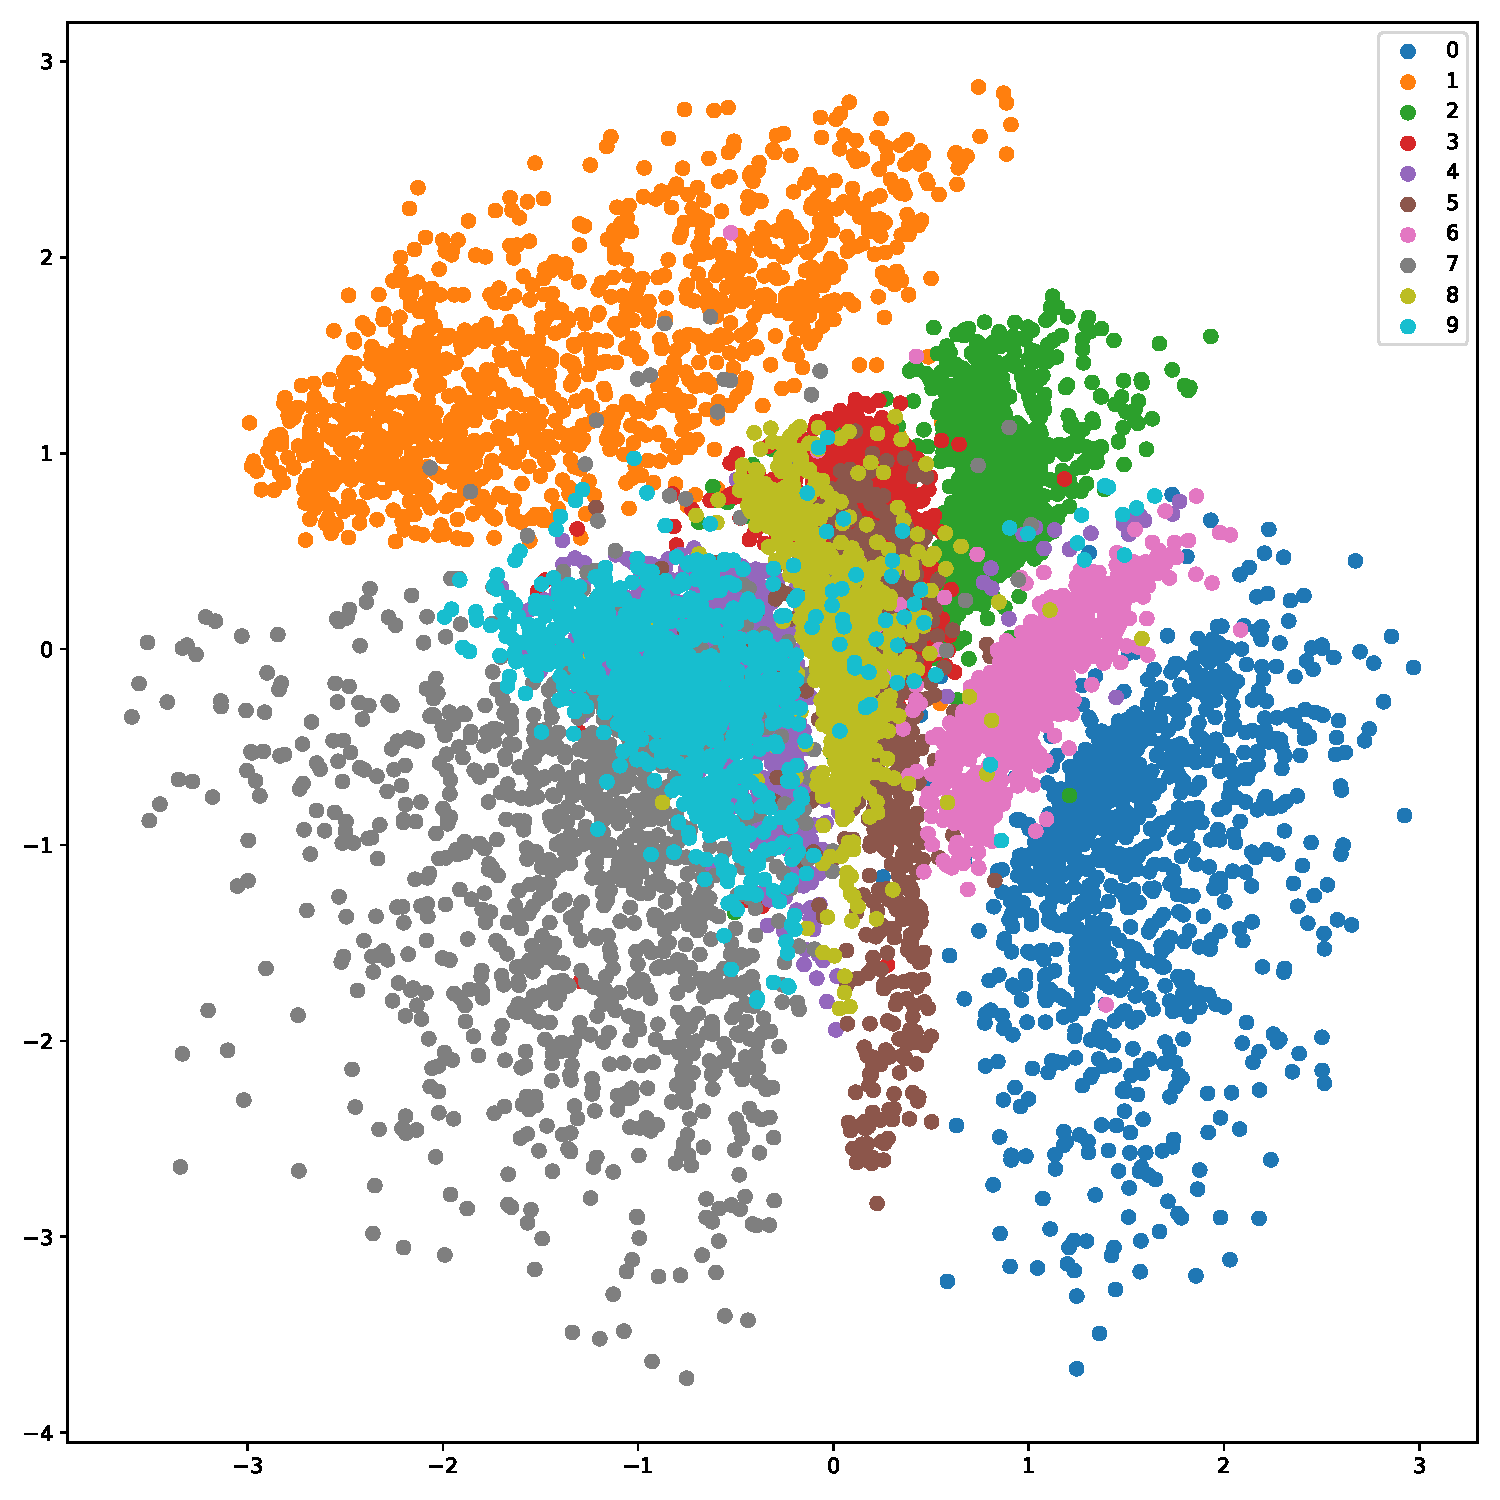
\includegraphics[width=\textwidth]{gfx/evaluation/feature_space/distributions_mnist}
  \caption{Latent Space}
  \label{fig:mnist_latent_space}
\end{subfigure}%
\begin{subfigure}{.5\textwidth}
  \centering
  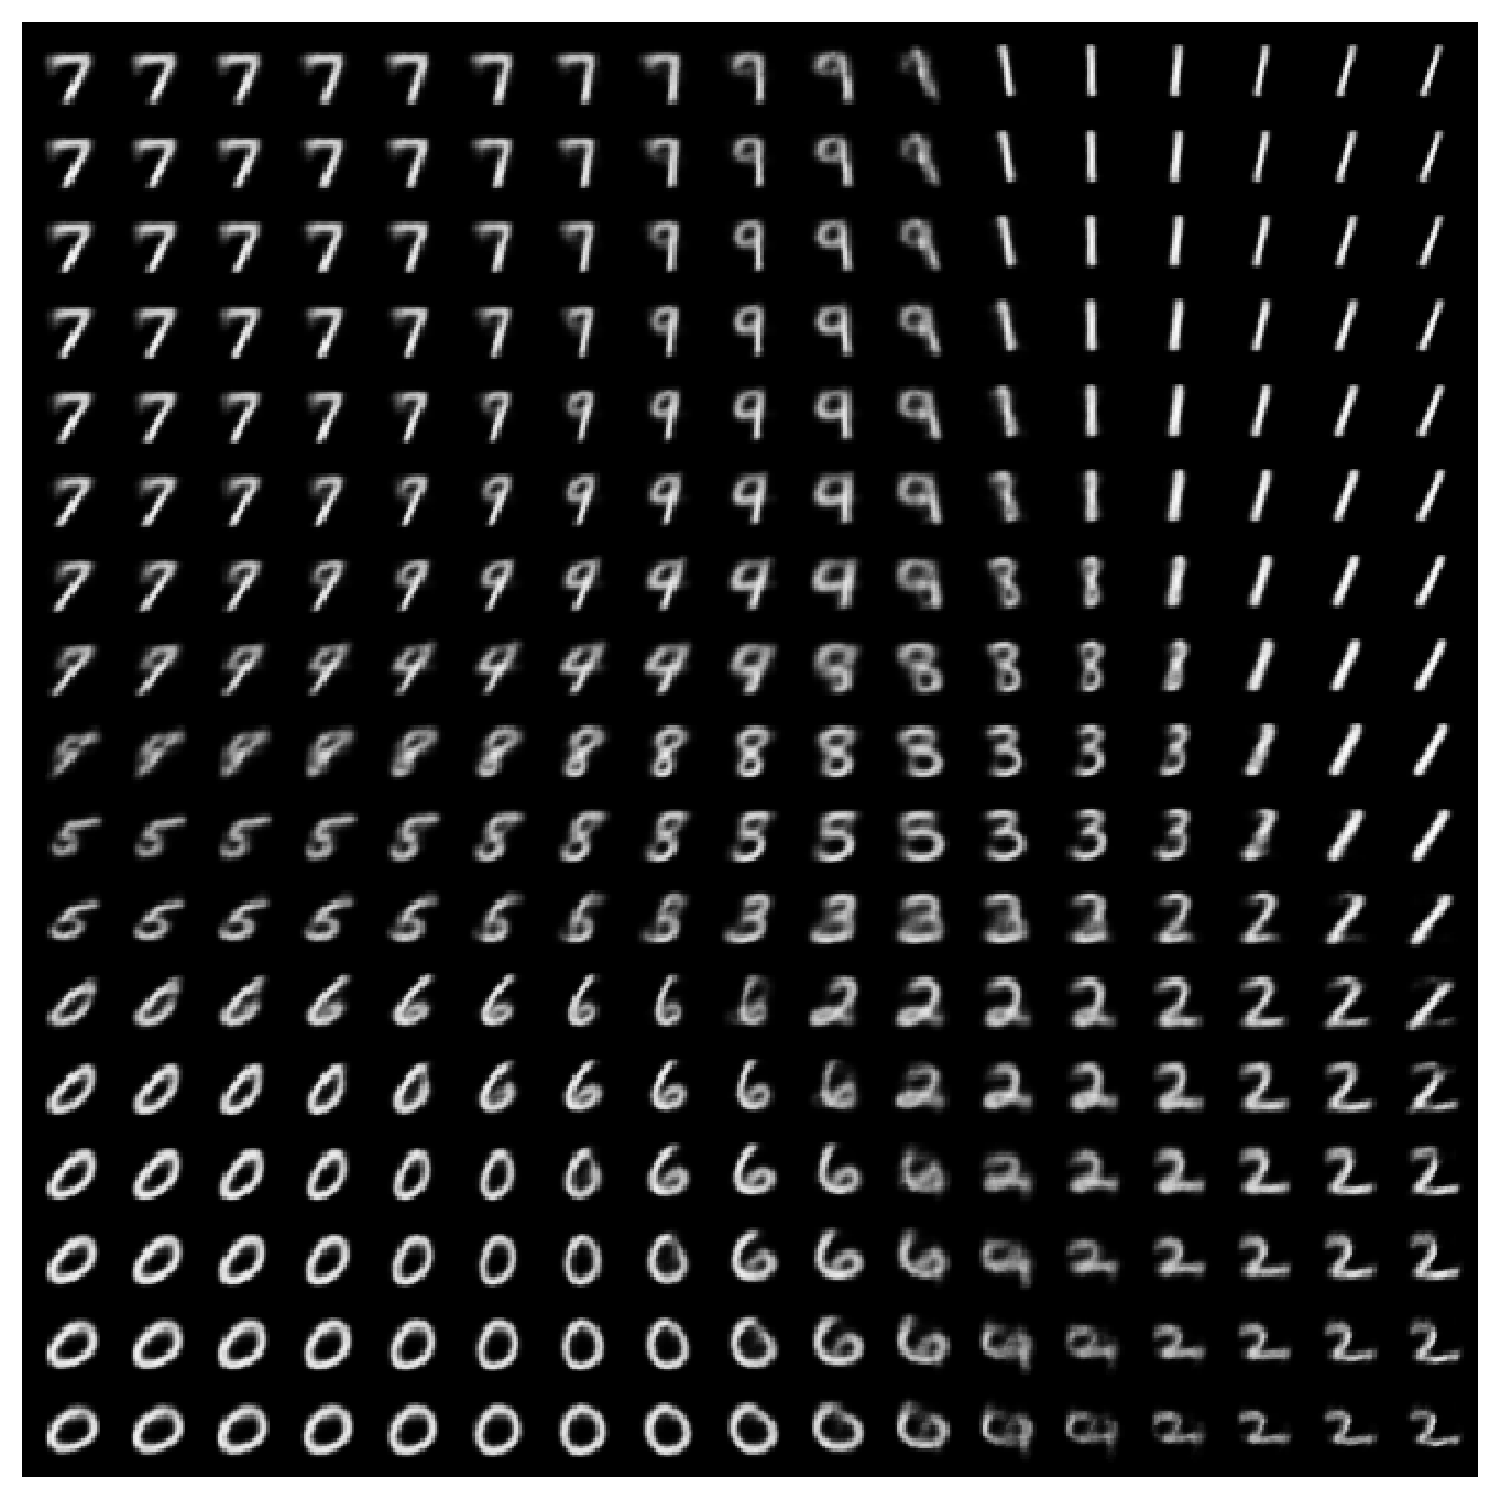
\includegraphics[width=\textwidth]{gfx/evaluation/feature_space/mnist_grid.pdf}
  \caption{Generierte Beispiele}
  \label{fig:mnist_reconstructions}
\end{subfigure}
\caption{(links) Der Latent Space eines Single-VAE auf dem Datensatz MNIST. Trainiert wurde mit $\beta = 0.5$. Zu sehen ist die klare Trennung der Klassen im äußeren Bereich. Nahe 0 sind die Klassen weniger deutlich getrennt. (rechts) Die Rekonstruktionen von Latent-Vektoren aus dem Intervall $(-3, 3)$. Auch hier sind die Rekonstruktionen im äußeren Bereich deutlich schärfer.}
\end{figure}

Abb. \ref{fig:mnist_reconstructions} zeigt die Rekonstruktionen von 2D Latent-Vektoren aus dem Intervall $(-3, 3)$ in beiden Dimensionen. Es ist dieselbe Trennung wie schon im Latent-Space sichtbar. An den Grenzen zwischen zwei Clustern sind außerdem Mischformen von Klassen zu sehen.

\begin{figure}[hbt]
  \centering
  
\includegraphics[width=\textwidth]{gfx/evaluation/feature_space/mnist_4}
  \caption{Rekonstruktionen verschiedener Original Ziffern 4 beim Single-VAE. Trainiert wurde mit $\beta = 0.5$. Zu sehen ist das Problem bei Überlappungen von Klassen im Latent-Space. Die Rekonstruktionen sind nicht eindeutig einer 4 oder 9 zuordbar, da durch die geringe Latent-Space Dimension ein zu hoher Informationsverlust mit einhergeht. Höheren Latent-Space Dimensionen verringern diesen Effekt.}
  \label{fig:mnist_recon_4}
\end{figure}

In Abb. \ref{fig:extrapolation_feature_space} ist die Funktionsweise des Interpolations- bzw. Extrapolations-Samplings gezeigt. Eine Erkenntnis ist, dass bei diesen Sampling Methoden immer garantiert ist, aus der Nähe von Originalbeispielen zu sampeln. Damit ergeben sich mehr plausible Rekonstruktionen. \\
\begin{figure}[hbt]
\centering
\begin{subfigure}{.5\textwidth}
  \centering
  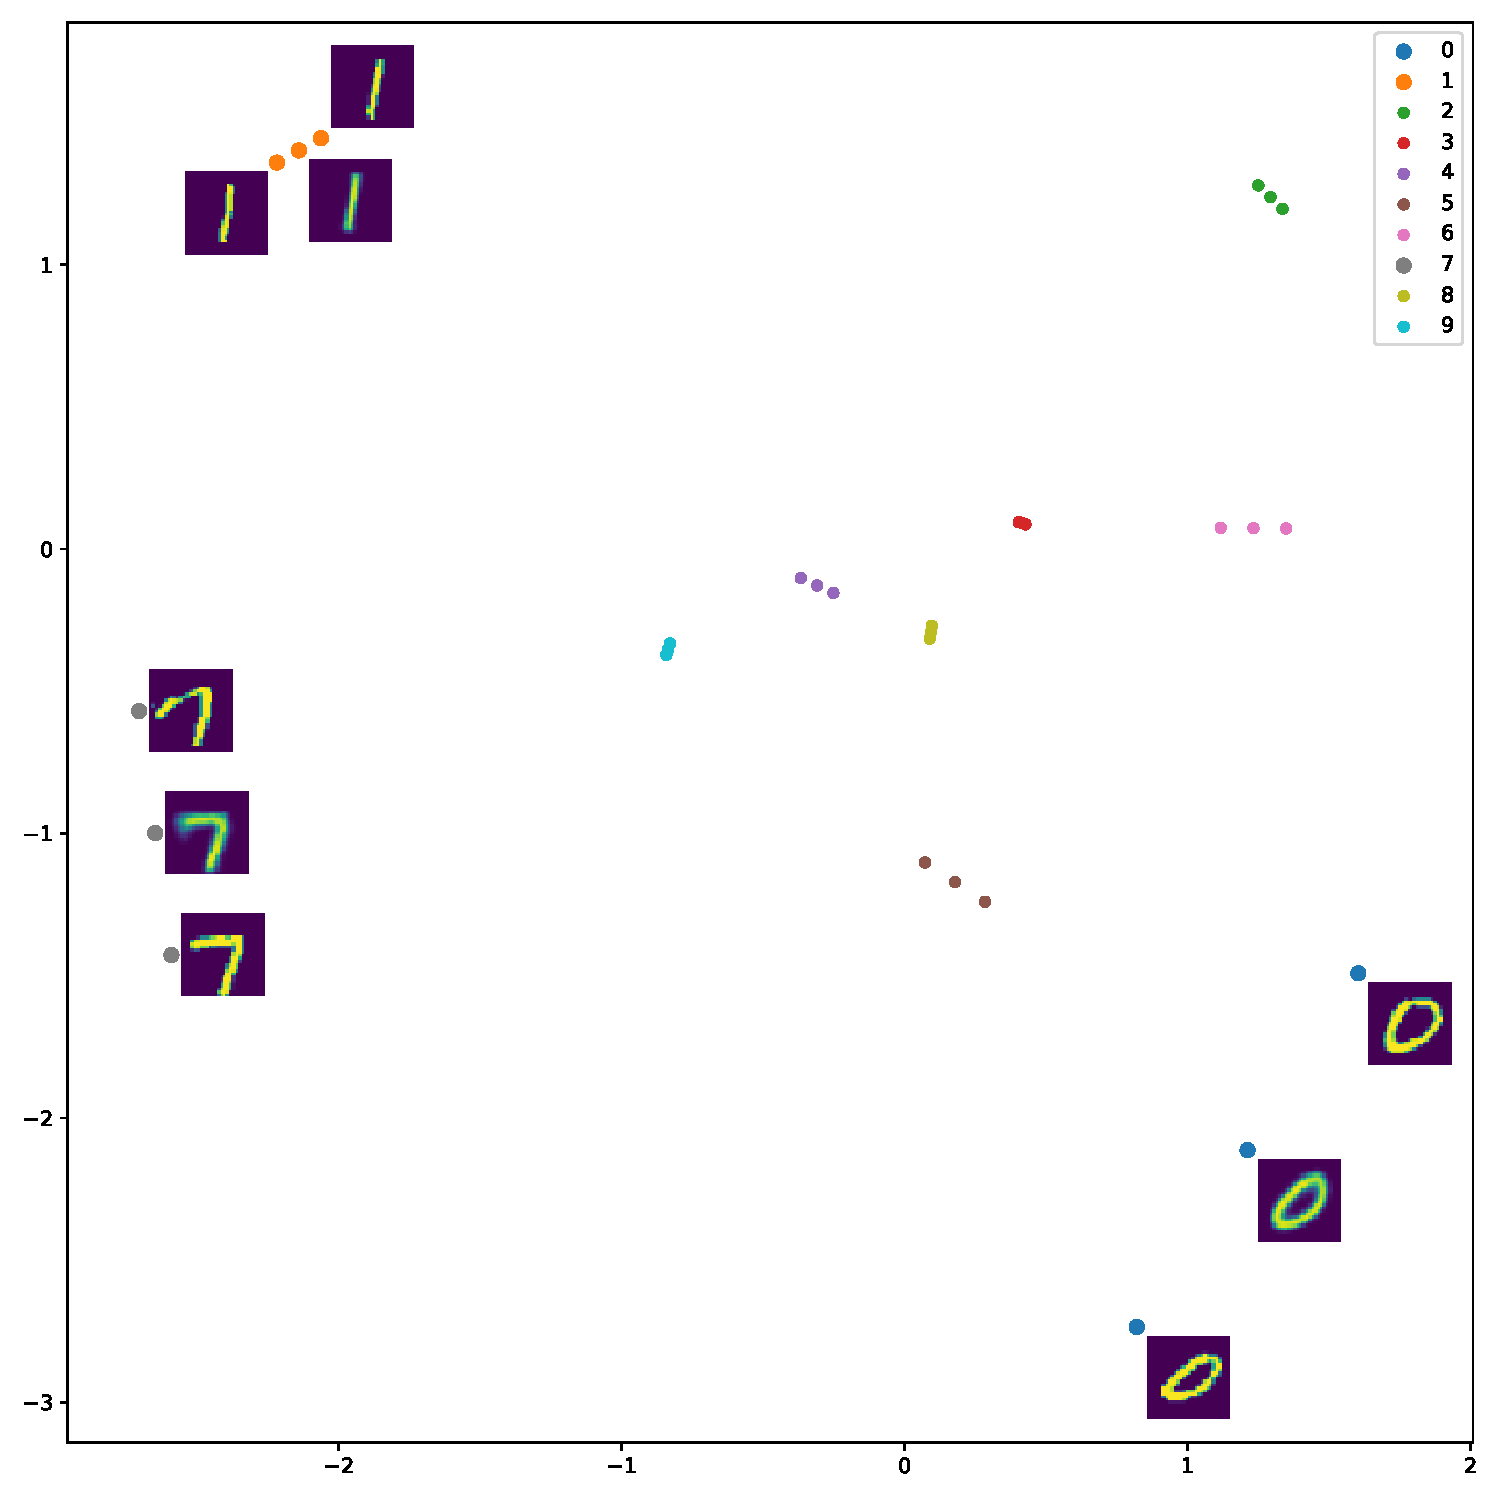
\includegraphics[width=\textwidth]{gfx/evaluation/feature_space/interpolation}
  \caption{Interpolation}
\end{subfigure}%
\begin{subfigure}{.5\textwidth}
  \centering
  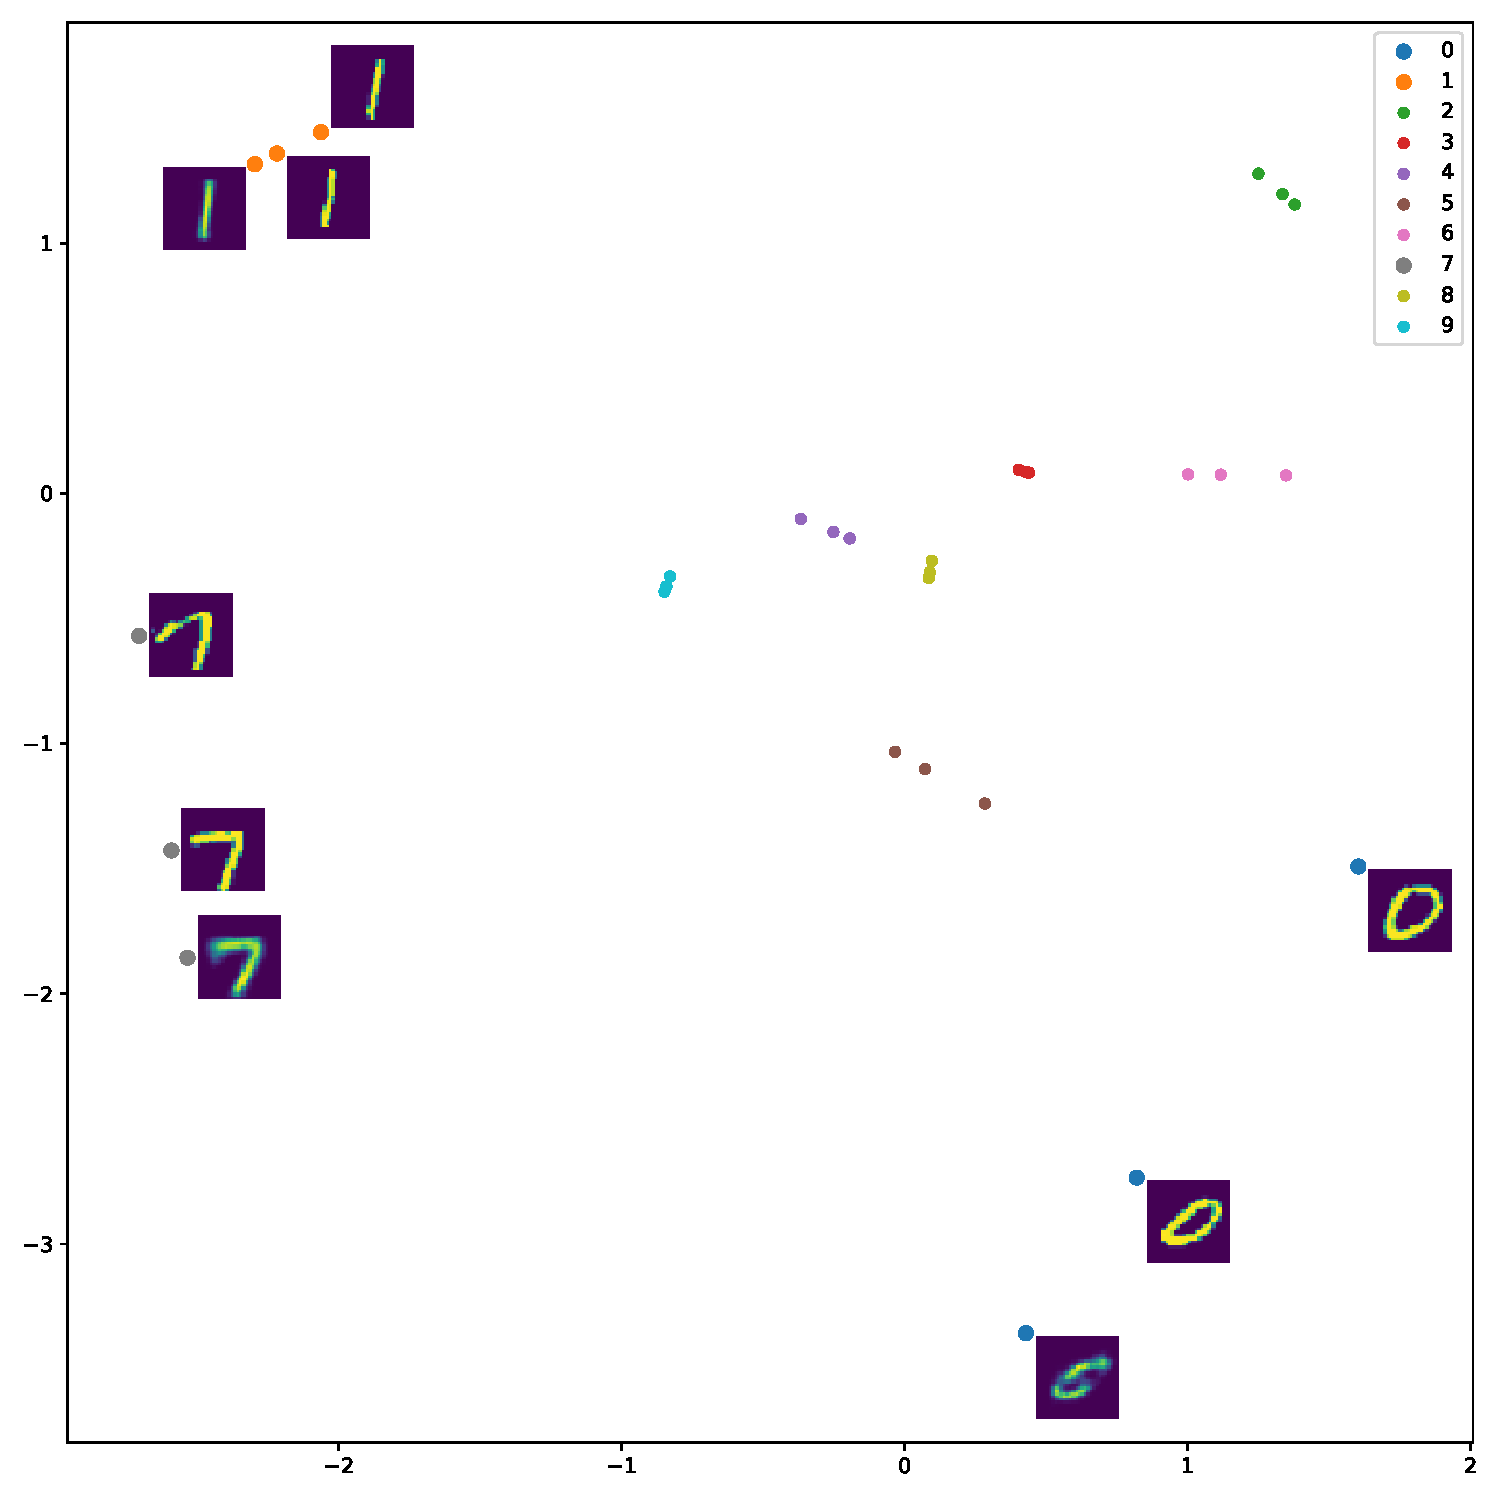
\includegraphics[width=\textwidth]{gfx/evaluation/feature_space/extrapolation}
  \caption{Extrapolation}
\end{subfigure}
\caption{Die Interpolations und Extrapolationsmethode. Zu sehen sind das Ergebnis der nächsten-Nachbar Suche im Latent-Space und der inter- / extrapolierte Punkt für jeweils ein Beispiel jeder Klasse. Der $\alpha$ Parameter wurde auf $0.5$ gesetzt, was bei einer Interpolation genau dem Mittelpunkt entspricht. Zusätzlich sind die Rekonstruktionen der korrespondierenden Punkte zu sehen.}
\label{fig:extrapolation_feature_space}
\end{figure}

In Abb. \ref{fig:mnist_beta_influence} wird der Einfluss des $\beta$ Faktors in der Fehlerfunktion des VAEs gezeigt. Für kleine $\beta$ Werte  ähnelt die Struktur des Latent-Space weniger einer Standardnormalverteilung. Er hat zwar immernoch eine probabilistische Form, welche durch das Sampling im Training (siehe Reparametrisierungstrick, Abschnitt \ref{sec:reparam_trick}) erreicht wird, die Latent-Vektoren weichen aber immer weiter von einem Erwartungswert 0 ab. Der KL-Term ist also essentiell wichtig, um eine bekannte Struktur im Latent-Space zu erzeugen. Gleichzeitig kann eine zu große Gewichtung dazu führen, dass der Latent-Space kollabiert und alle Eingaben auf Erwartungswert 0 und Varianz 1 abbildet. Für Datensätze mit eindeutigen Klassen ist dies von großem Nachteil, da die Merkmale nun voneinander entkoppelt sind (\textit{Disentanglement}, siehe \cite{Higgins2017}). Der Latent-Vektor verliert die Informationen über seine eindeutigen Merkmale. Für Multi-Label Klassifikation kann sich diese Eigenschaft jedoch zu Nutze gemacht werden, um gezielt Merkmale zu dekorrelieren. In den Rekonstruktionen in Abb. \ref{fig:mnist_recon_beta_influence} sehen wir, dass eine größere Gewichtung der KL-Divergenz ein verschwommenere Rekonstruktion mit sich bringt.
%\begin{figure}[H]
%  \centering
%  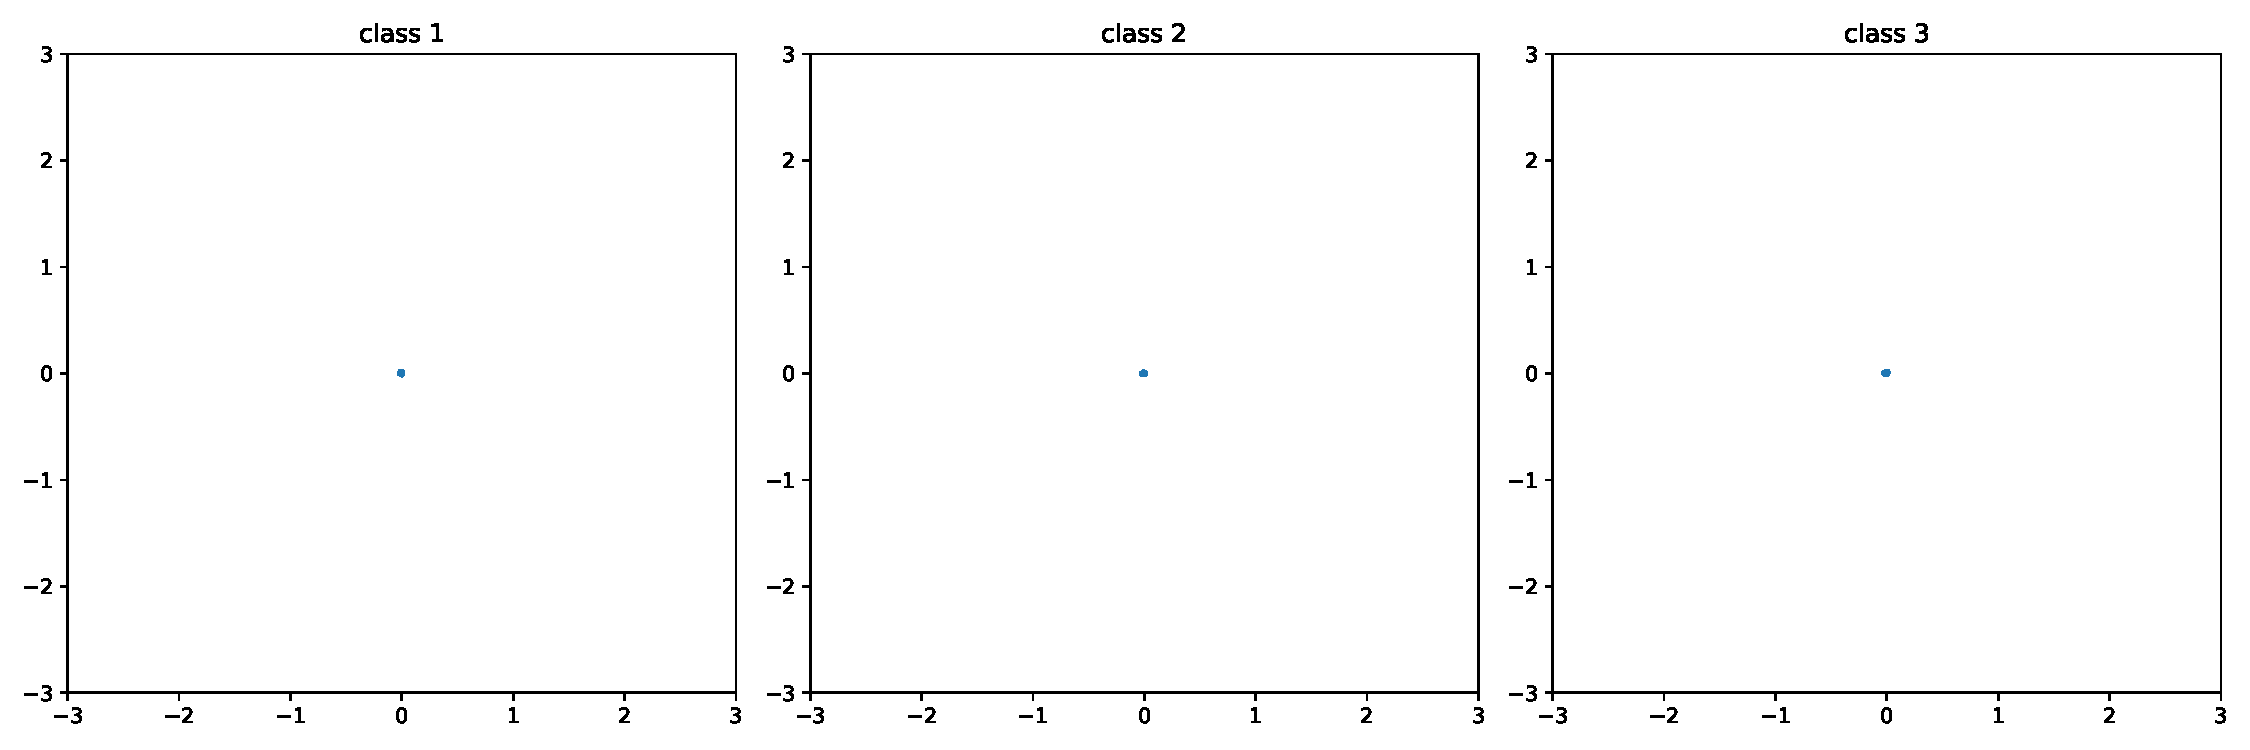
\includegraphics[width=.7\textwidth]{gfx/evaluation/feature_space/thyroid_collapse}
%  \caption{Latent-Space der klassenweisen Multi-VAEs auf dem "thyroid" Datensatzes mit $\beta=1.0$. Alle Eingabebeispiele werden auf den Latent-Vektor 0 abgebildet.}
%  \label{fig:thyroid_collapse}
%\end{figure}

\begin{figure}[H]
\centering
\begin{subfigure}{.28\textwidth}
  \centering
  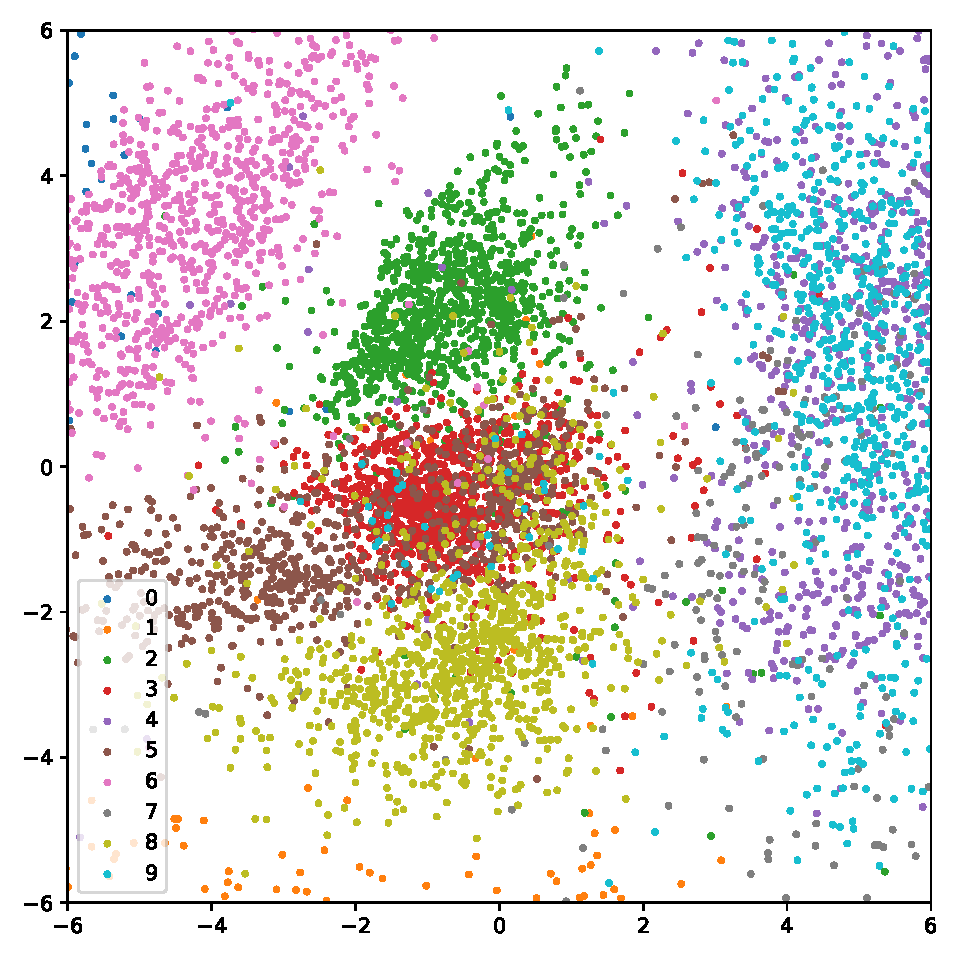
\includegraphics[width=\textwidth]{gfx/evaluation/feature_space/beta=0.001.pdf}
  \caption{$\beta = 0.001$}
\end{subfigure}
\begin{subfigure}{.28\textwidth}
  \centering
  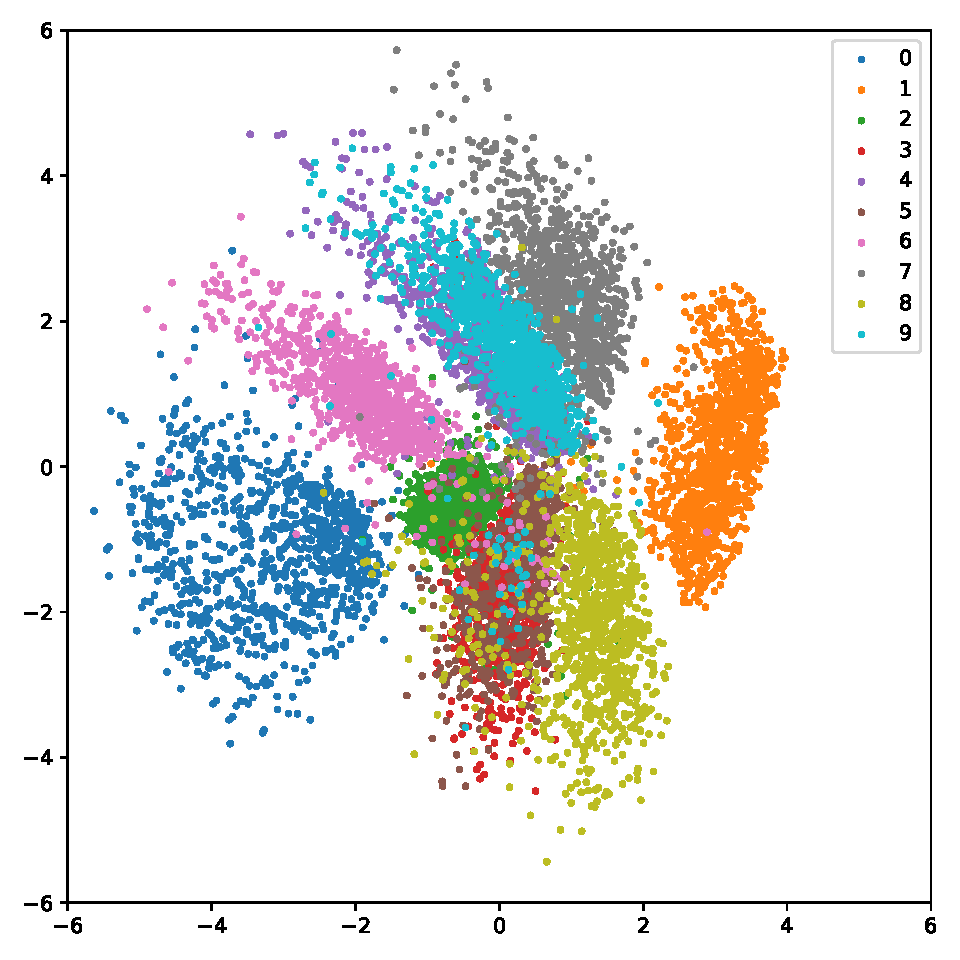
\includegraphics[width=\textwidth]{gfx/evaluation/feature_space/beta=0.1.pdf}
  \caption{$\beta = 0.1$}
\end{subfigure}
\begin{subfigure}{.28\textwidth}
  \centering
  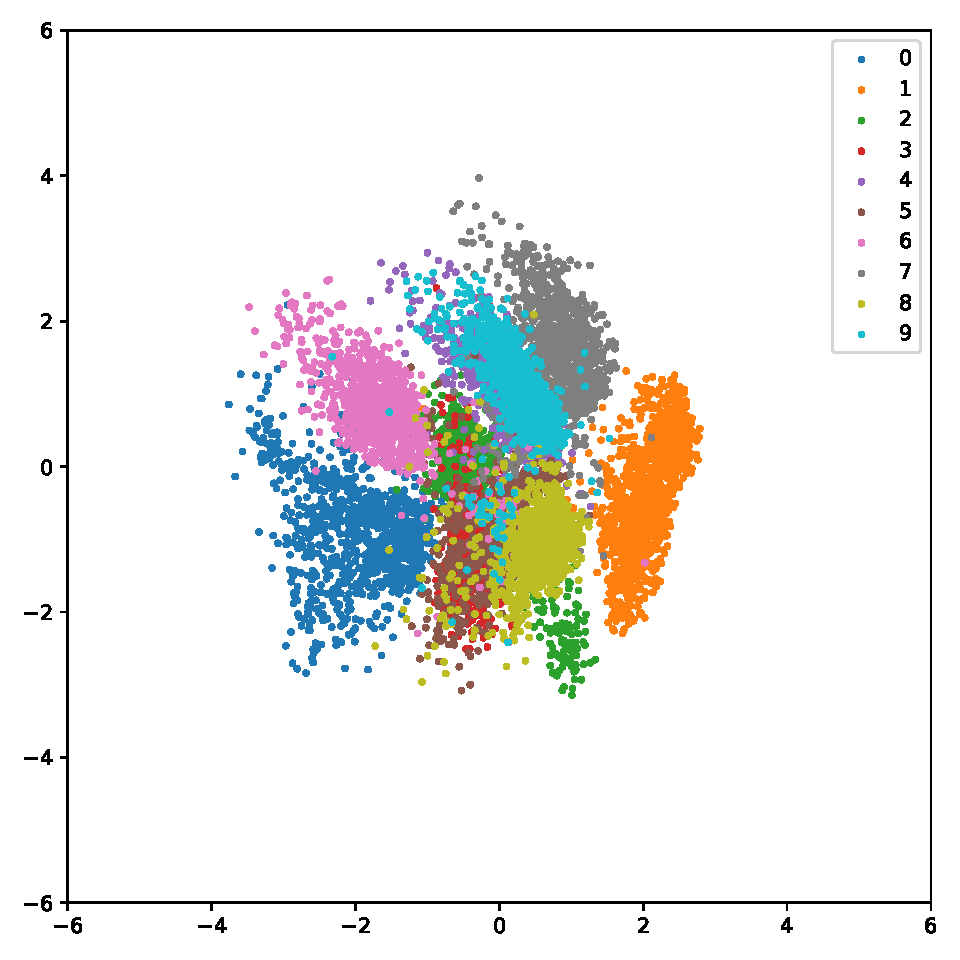
\includegraphics[width=\textwidth]{gfx/evaluation/feature_space/beta=0.5.pdf}
  \caption{$\beta = 0.5$}
\end{subfigure}
\begin{subfigure}{.28\textwidth}
  \centering
  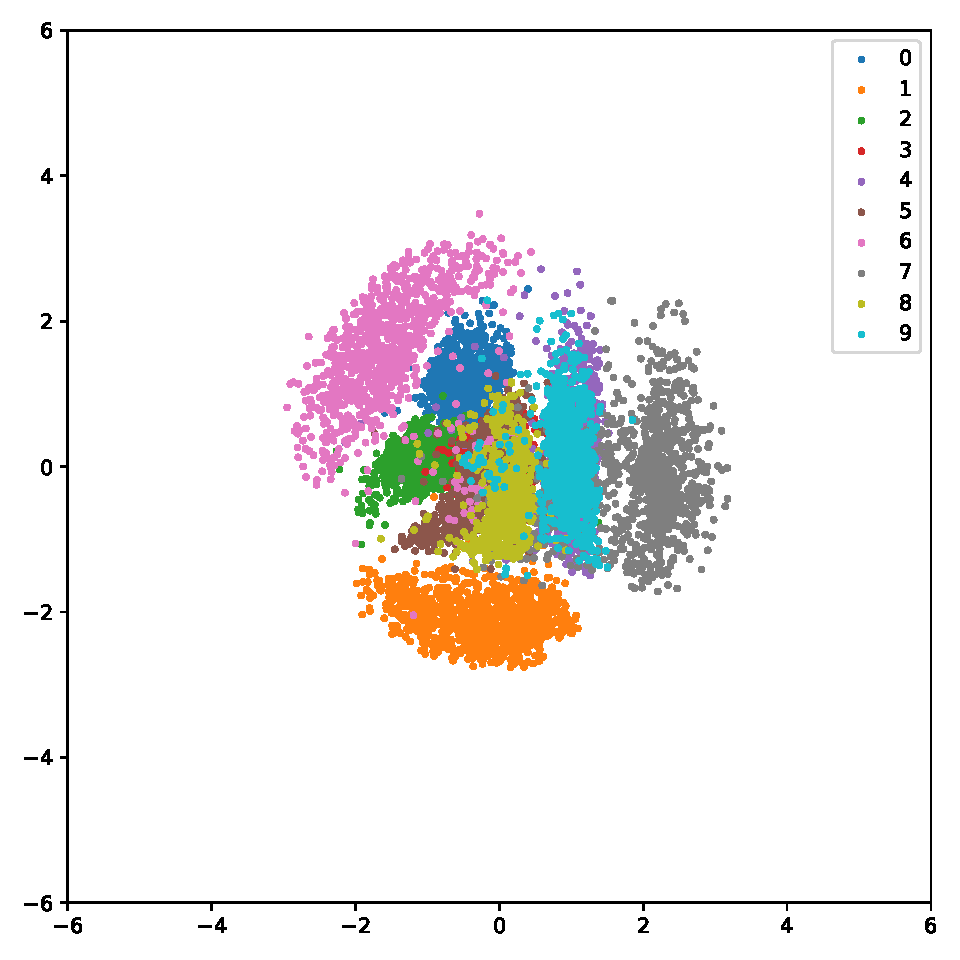
\includegraphics[width=\textwidth]{gfx/evaluation/feature_space/beta=1.0.pdf}
  \caption{$\beta = 1.0$}
\end{subfigure}
\begin{subfigure}{.28\textwidth}
  \centering
  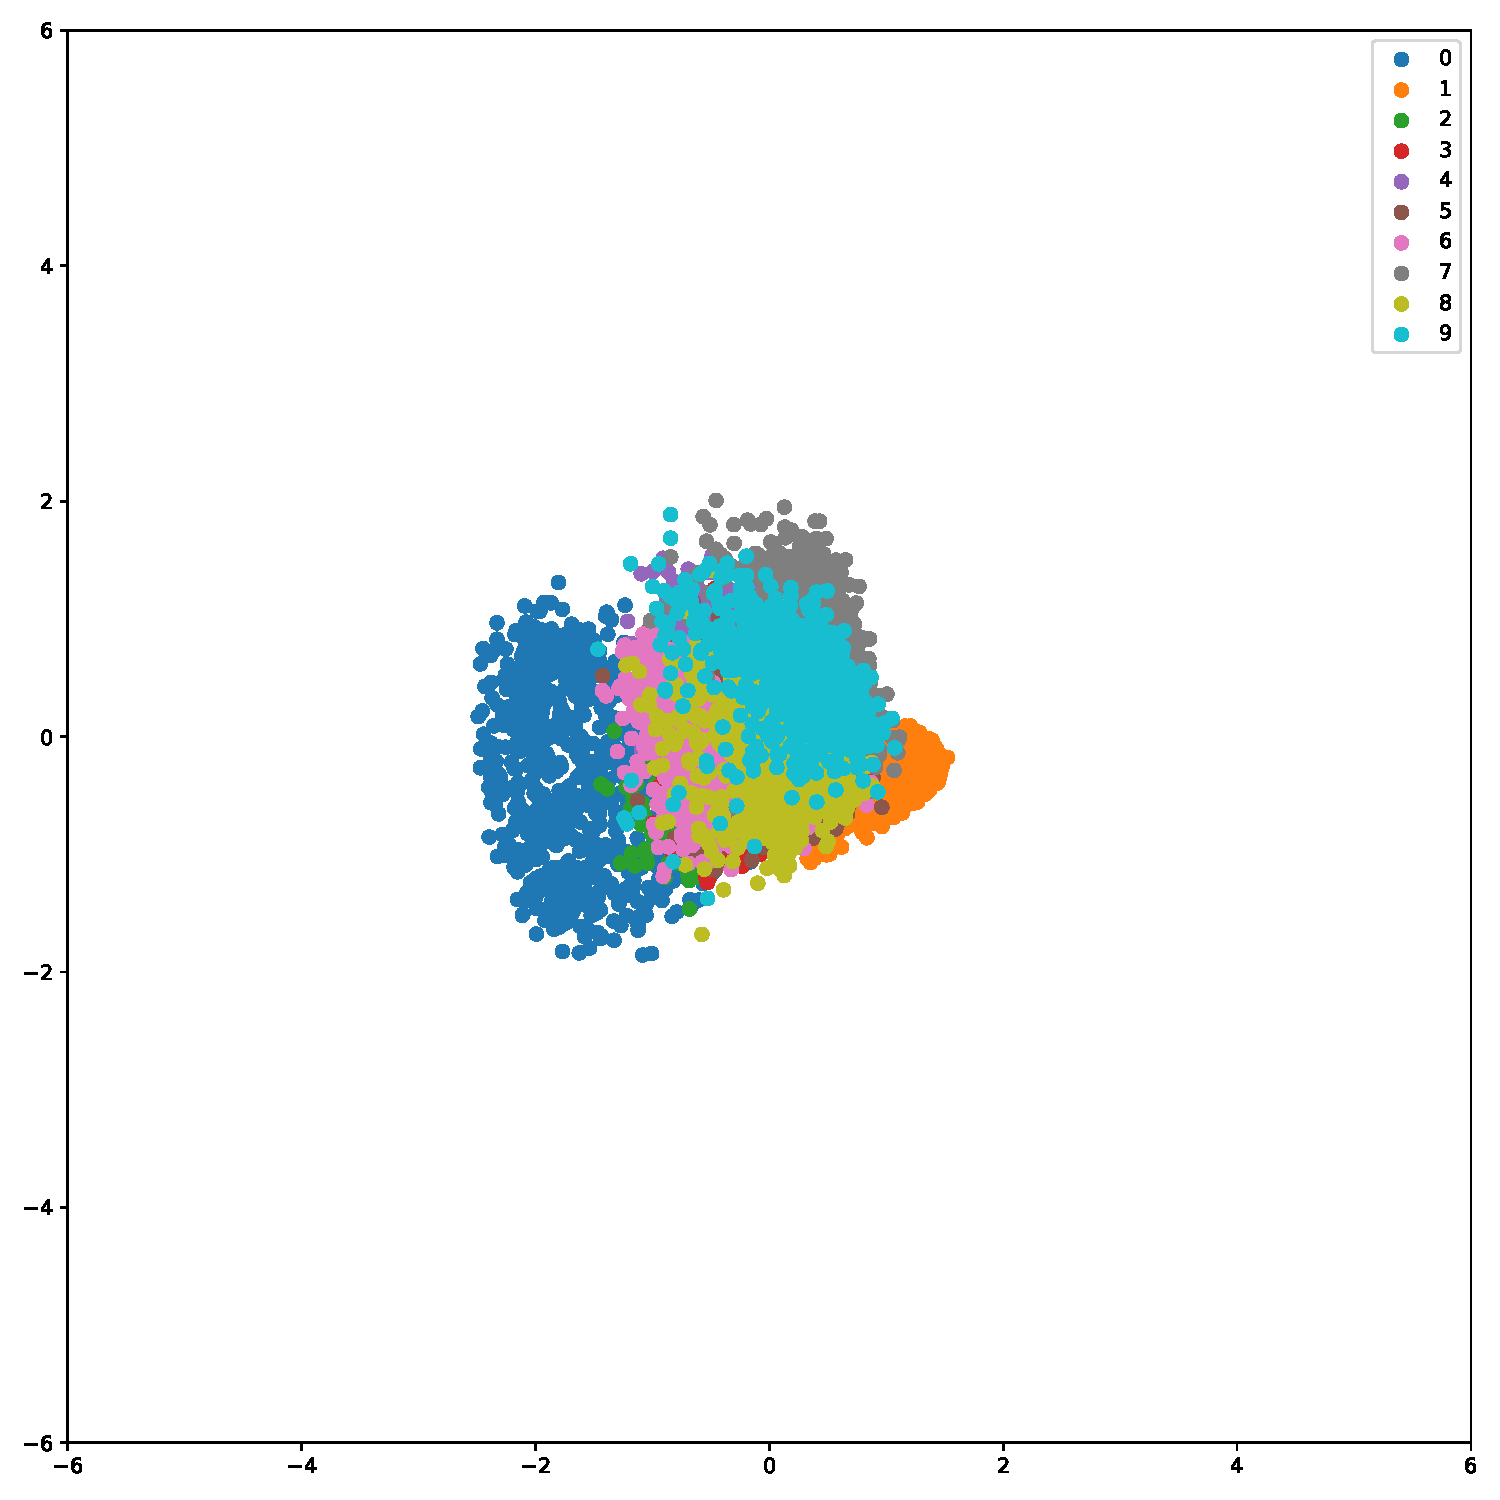
\includegraphics[width=\textwidth]{gfx/evaluation/feature_space/beta=10.0.pdf}
  \caption{$\beta = 10.0$}
\end{subfigure}
\caption{Der Latent-Space eines Single-VAEs (MNIST) für verschiedene Werte von $\beta$. Erkennbar ist, dass zu kleine Werte für $\beta$ weniger Annahmen über die Latent-Vektoren ermöglichen. Zu große Werte haben dagegen einen vollständigen Strukturverlust zur Folge.}
\label{fig:mnist_beta_influence}
\end{figure}

\begin{figure}[H]
  \centering
  
\includegraphics[width=1.3\textwidth]{gfx/evaluation/feature_space/mnist_beta=50.0}
  
\includegraphics[width=1.3\textwidth]{gfx/evaluation/feature_space/mnist_beta=1.0}
  
\includegraphics[width=1.3\textwidth]{gfx/evaluation/feature_space/mnist_beta=norm}
  \caption{Rekonstruktionen zufälliger MNIST Beispiele eines Single-VAEs. Höhere Werte für $\beta$ haben deutlich unschärfere rekonstruierte Bilder zur Folge. Extrem kleine Werte beeinträchtigen die Rekonstruktionsqualität dagegen nicht.}
  \label{fig:mnist_recon_beta_influence}
\end{figure}

Für numerische Daten in den PROBEN1 Datensätzen hat es sich als außerordentlich schwierig erwiesen, geeignete Hyperparameter für einen strukturierten Latent-Space zu finden. In vielen Fällen kollabierte der Latent-Space schon für Werte für $\beta > 0.5$. Ein Grund dafür ist das Verhältnis des BCE-Fehlers zur KL-Divergenz. Für MNIST ist der BCE-Fehler entsprechend groß, da die Bildgröße mit $28 \times 28$ Pixeln einen hohen BCE-Fehler bewirkt (vgl. Reduktion des BCE-Fehlers, Abschnitt \ref{sec:beta_vae}). Im Falle von PROBEN1 jedoch ist die Eingabe nur 8-60 dimensional. Über $\beta$-Normalisierung konnte diesem Problem in den meisten Fällen entgegen gewirkt werden. Bei numerischen Daten hatten auch Batch-Größen von über 32 einen negativen Effekt auf die Struktur des Latent-Spaces. \\

Ein weiteres Problem bei den numerischen Daten des PROBEN1 Datensatzes sind die diskreten Attribute. In Abb. \ref{fig:discrete_problem} ist eine Clusterbildung im Latent-Space zu erkennen.
\begin{figure}[H]
  \centering
  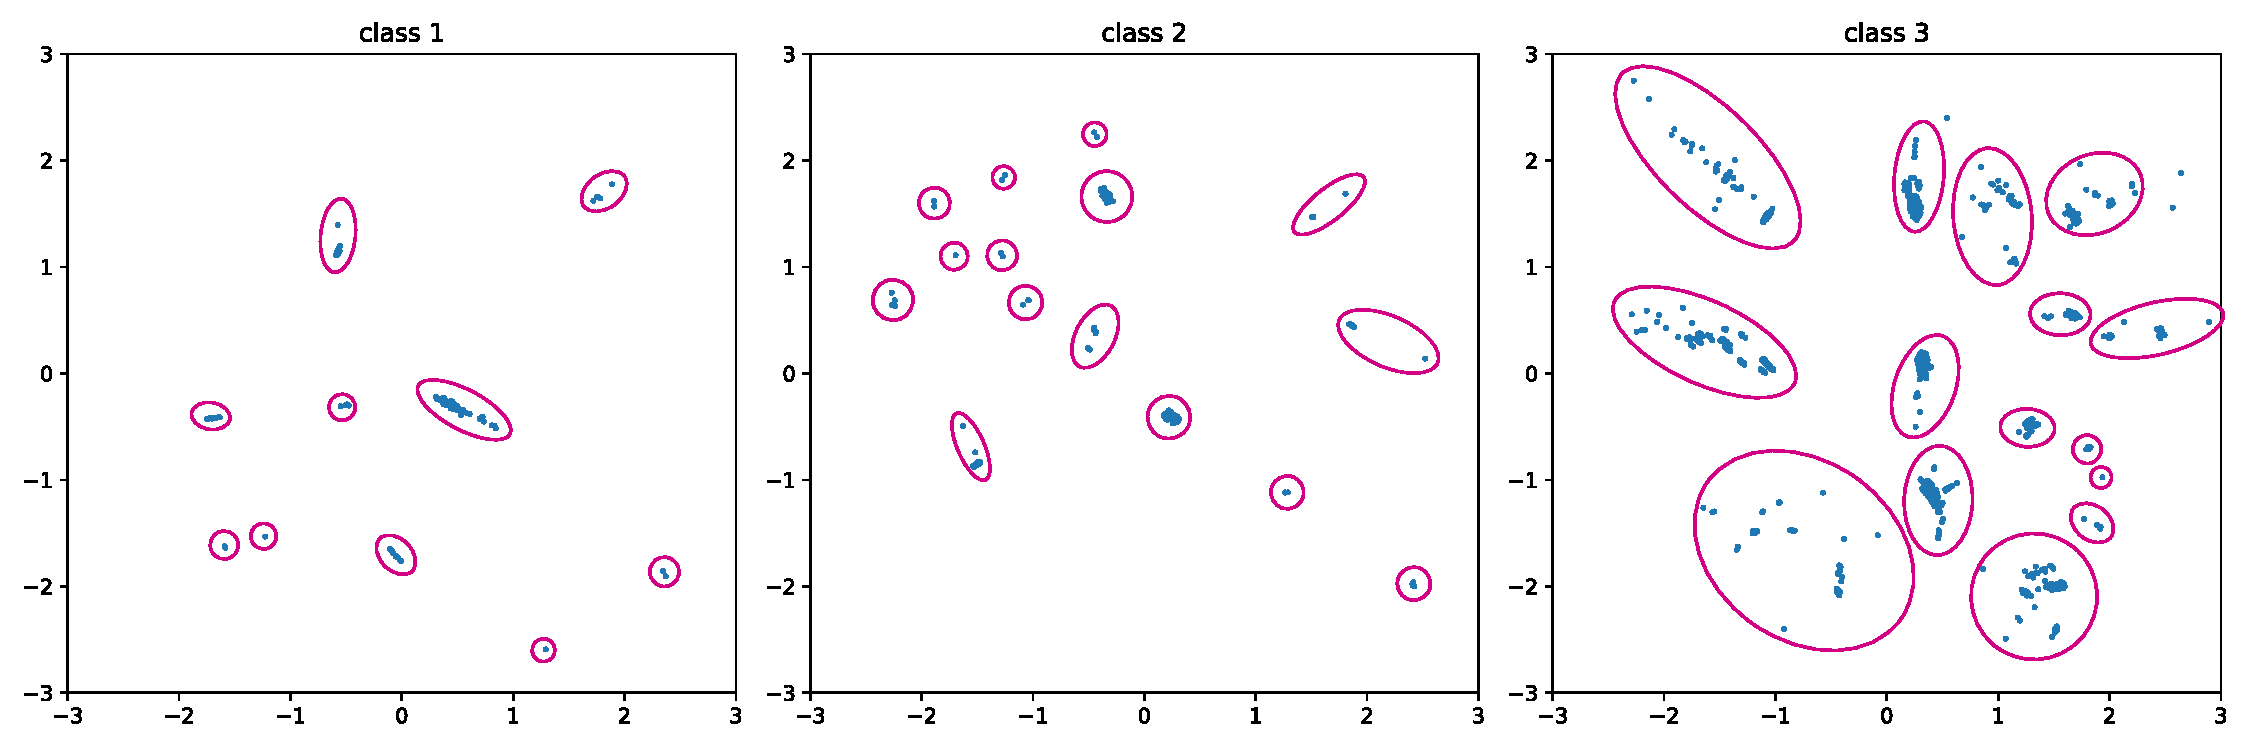
\includegraphics[width=\textwidth]{gfx/evaluation/feature_space/discrete_problem_with_cluster}
  \caption{Latent-Spaces der Klassenweisen VAEs auf dem "thyroid" Datensatz. Der Datensatz besitzt 15 diskrete Attribute und 6 kontinuierliche Attribute. Besonders im Latent-Space zur Klasse 2 führen diese 15 diskreten Attribute zu 15 Clustern.}
  \label{fig:discrete_problem}
\end{figure}
Es zeigt sich eine Relation zwischen der Anzahl an diskreten Attributen und Clustern. Für jedes Attribut entsteht ein Teil-Cluster für jeden Wert aus dem Wertebereich des Attributes. In der Abbildung ist dies besonders in Klasse 2 zu sehen. Man beachte, dass die Attribute des Datensatzes "thyroid" alle binär sind, also 2 Teil-Cluster erkennbar sind. Im Latent-Space der Klasse 3 ist dieses Clustering weniger scharf, aber ebenfalls erkennbar. Grund hierfür ist, dass die Klasse 3 insgesamt 5333 Beispiele, die Klasse 2 dagegen nur 294 Beispiele enthält. So wird der Zwischenraum innerhalb der Cluster in Klasse 3 mehr exploriert. Dieses Clustering ist problematisch für das Generieren neuer Beispiele. Die Grundannahme für das Sampling im Latent-Space besteht darin, dass die Verteilung ähnlich zu einer Standard Normalverteilung ist. Erzielt die KL-Divergenz Regularisierung diese Struktur nicht, so werden Rekonstruktionen erzeugt, welche stark verrauscht sind. Dies hat einen negativen Einfluss auf das Training eines Klassifikators auf diesen generierten Daten.




\section{PROBEN1}
Die Experimente auf den PROBEN1 Datensätzen stellten sich als sehr Hyperparameter sensitiv heraus. So hatte beispielsweise der $\beta$ Parameter, die Batch-Größe des VAEs und die Trainingsdauer des VAEs einen erheblichen Einfluss auf die Resultate. Eine Erkenntnis war, dass die Gefahr des Overfittings beim VAE relativ gering ist. Generell galt: Je länger der VAE trainiert wurde, desto besser wurden die Rekonstruktionen und damit die Ergebnisse im Training mit generierten Daten. Ab ca. 6000 Trainingsschritten (je nach Größe des Datensatzes), verbessert sich die Qualität der Rekonstruktionen nicht mehr. Dies ist nicht überraschend, da Regularisierung des KL-Terms und das Sampling während des Trainings Overfitting verhindern.
In den Experimenten zu PROBEN1 wurde sowohl der Multi-VAE, als auch Single-VAE auf der selben Datenmenge trainiert. Hierbei stellte sich heraus, dass sowohl auf dem gesamten Datensatz, als auch im Few-Shot Szenario der Single-VAE Ansatz keine Verbesserung in der Klassifikation erzielen konnte. Grund dafür ist dass die Eigenschaft des selbst-überwachten Lernens nicht durch zusätzliche nicht-annotierte Daten ausgenutzt werden kann. Ebenso übertraf das zufällige Sampling aus der Normalverteilung $\cN(0, 1)$ die anderen Sampling Methoden im Multi-VAE Fall. Die hier beschriebenen Ergebnisse beschränken sich daher auf den Multi-VAE Ansatz mit Sampling aus der Standardnormalverteilung.

\subsection{Performanz auf dem gesamtem Datensatz}
Für das Training eines Klassifikators auf jeweils dem gesamten Datensatz konnten Verbesserungen des \textit{weighted-f-score} in fast allen Datensätzen erzielt werden. Für das Training mit generierten Daten wurden genauso viele echte Trainingsbeispiele wie generierte benutzt. Mehr generierte Daten hinzuzunehmen, erzielte auf diesen Datensätze keine Verbesserungen. Die Anzahl an Trainingsschritten für den VAE und die Sensitivität des Generative Classifiers wurde jeweils an den Datensatz angepasst. Alle VAEs wurden mit Latent-Space Dimension $d = 2$ trainiert. Es stellte sich heraus, dass eine höhere Dimension auf diesen Datensätzen keine Verbesserung zur Folge hatte. Abb. \ref{tab:eval_proben1_all} zeigt den \textit{weighted-f-score} des Klassifikationsnetzwerks auf den Originaldaten (Baseline), den generierten Daten (VAE) und den gefilterten Daten des Generative Classifiers (VAE + GC). \\

Es ist eine leichte Verbesserung des F-Scores für die mit VAE Daten trainierten Modelle sichtbar. Die höchste Verbesserung konnte im Datensatz "horse" mit 0.016 erzielt werden. Die Datensätze "thyroid" und "geneN" erreichten eine Verbesserung nur, wenn kein Balancing erfolgte. Das Mischen der klassenweisen Datensätze führte hierbei zu einem höheren F-Score. In den anderen Datensätzen konnten bessere Ergebnisse erzielt werden, wenn nicht gemischt, dafür aber die kleineren Klassen ausbalanciert wurden. Die identischen F-Score Werte für den Datensatz "glass" lassen sich dadurch begründen, dass der F-Score für 2 der 3 Seeds bei $1.00$ lag, die Baseline also bereits nahezu fehlerfrei war. Generell ist die Verbesserung mit generierten Daten sehr gering und hängt stark vom Datensatz und der Wahl des Seeds ab. Es ist nicht auszuschließen, dass Zufalls Effekte hier eine Rolle spielen. imbalancierte Datensätze wie "thyroid" erzielen tendenziell weniger Verbesserungen mit dem VAE Ansatz. Der Generative Classifier führt in einigen Fällen zu einem höheren F-Score als der VAE ohne GC. Jedoch fiel beim Trainieren auf, dass je nach Seed die Sensitivität für "schlechte" Beispiele unterschiedlich hoch war. Seed übergreifend Hyperparameter zu finden, erwies sich als äußerst schwierig. \\

Im Vergleich zu den generativen Modellen der Autoren \cite{Moreno-Barea2020} liefert der hier verwendete VAE Ansatz eine geringere Modellgüte. Insbesondere die dort verwendeten Generative-Adversarial-Networks erzielten bessere Resultate.

\begin{table}[hbt]
\centering
\scalebox{.8}{\begin{tabular}{l|c|c|c|c}
\toprule
Datensatz      & $\beta$             & Baseline & VAE            & VAE + GC       \\ \hline
card           & norm=0.133          & 0.871    & 0.873          & 0.869          \\
balance: Ja    & 0.5                 & 0.871    & 0.868          & 0.864          \\
Mix data: Nein & \textbf{1.0}        & 0.871    & \textbf{0.876} & 0.871          \\ \midrule
diabetes       & norm=0.25           & 0.823    & 0.831          & 0.826          \\
balance: Ja    & 0.5                 & 0.823    & 0.830          & 0.822          \\
Mix data: Nein & \textbf{1.0}        & 0.823    & 0.827          & \textbf{0.833} \\ \midrule
geneN          & norm=0.033          & 0.813    & 0.802          & 0.814          \\
balance: Nein  & \textbf{0.5}        & 0.813    & \textbf{0.818} & 0.813          \\
Mix data: Ja   & 1.0                 & 0.813    & 0.812          & 0.813          \\ \midrule
glass          & norm=0.222          & 0.985    & 0.977          & 0.985          \\
balance: Ja    & 0.5                 & 0.985    & 0.977          & 0.985          \\
Mix data: Nein & 1.0                 & 0.985    & 0.984          & 0.985          \\ \midrule
horse          & \textbf{norm=0.1}   & 0.828    & 0.837          & \textbf{0.844} \\
balance: Ja    & 0.5                 & 0.828    & 0.833          & 0.835          \\
Mix data: Nein & 1.0                 & 0.828    & 0.836          & 0.828          \\ \midrule
thyroid        & \textbf{norm=0.095} & 0.954    & 0.952          & \textbf{0.956} \\
balance: Nein  & \textbf{0.5}        & 0.954    & 0.927          & \textbf{0.956} \\
Mix data: Ja   & 1.0                 & 0.954    & 0.925          & 0.954          \\
\bottomrule
\end{tabular}}
\caption{F-Scores auf den PROBEN1 Datensätzen. Das beste Ergebnis ist jeweils \textbf{fett} gedruckt. Bis auf den "glass" Datensatz verbessert sich der F-Score durch den VAE um ca. $0.007$. Es wurden 3 verschiedene Werte für $\beta$ getestet: $1.0, 0.5$ und $1.0$ mit $\beta$-Normalisation (mit norm angegeben). Höhere Werte für $\beta$ führten zum Kollaps im Latent-Space und daraus resultierend schlechterer Güte.}
\label{tab:eval_proben1_all}
\end{table}


\subsection{Few-Shot Szenario}
Abbildung \ref{plt:thyroid-few-shot} zeigt, dass die Verbesserung im F-Score mit zunehmender Anzahl an Trainingsbeispielen abnimmt. Ab 50 Beispielen pro Klasse ist sogar keine Verbesserung mehr sichtbar. Der Baseline Score liegt dann schon entsprechend hoch. Es scheint, als würden die verrauschten Beispiele, die der VAE generiert, die Klassifikationsaufgabe erschweren. Lediglich bei sehr wenig Beispielen pro Klasse sind die Beispiele hilfreich für die Klassifikation. Der Generative Classifier scheint das Ergebnis nicht konsequent zu verbessern.

\begin{table}[H]
\centering
\scalebox{.8}{\begin{tabular}{l|l|c|c|c}
\toprule
\# Trainingsbeispiele & \# Generierte Beispiele & Baseline       & VAE            & VAE + GC       \\ \hline
5                     & 5                       & 0.619          & \textbf{0.693} & 0.675          \\
10                    & 10                      & 0.727          & \textbf{0.778} & 0.761          \\
20                    & 20                      & 0.735          & 0.753          & \textbf{0.778} \\
30                    & 30                      & 0.772          & 0.786          & \textbf{0.796} \\
50                    & 50                      & \textbf{0.818} & 0.815          & 0.808          \\
100                   & 100                     & \textbf{0.935} & 0.927          & 0.922          \\
\bottomrule
\end{tabular}}
\caption{Der F-Score auf dem Datensatz "thyroid" im Few-Shot Szenario. Für kleine Trainingsgrößen ergibt sich ein verbesserte Wert von bis zu $0.074$. Die Verbesserung nimmt mit der Anzahl originaler Trainingsbeispiele ab.}
\label{tab:eval_thyroid_few_shot}
\end{table}

\begin{figure}[H]
\centering
\begin{tikzpicture}
\begin{axis}
[
  width=.6\textwidth,
  height = 4cm,
  symbolic x coords={5,10,20,30,50,100},
  xtick={5,10,20,30,50,100},
  xlabel={\# Beispiele pro Klasse},
  ylabel={$\Delta$ F-Score},
  grid,
  legend pos=south west,
]

\addplot[blue, mark=* , solid] table[col sep=comma, x=n_originals, y=improvement]{data/evaluation/thyroid-few-shot.csv};
\addlegendentry{F1-Increase}

\end{axis}
\end{tikzpicture}
\caption{Differenz des Baseline F-Scores und des Multi-VAEs auf dem Datensatz "thyroid" im Few-Shot-Szenario. Es wurde jeweils der höchste Wert von VAE und VAE + GC verwendet}
\label{plt:thyroid-few-shot}
\end{figure}

%\begin{table}[hbt]
%\centering
%\begin{tabular}{l|l|c|c|c}
%\toprule
%\# Trainingsbeispiele & \# Generierte Beispiele & Baseline       & VAE            & VAE + GC       \\ \hline
%2                     & 2                       & \textbf{0.657} & 0.652          & 0.652          \\
%3                     & 3                       & 0.782          & \textbf{0.788} & 0.756          \\
%4                     & 4                       & 0.748          & 0.753          & \textbf{0.758} \\
%5                     & 5                       & \textbf{0.740} & 0.721          & 0.724          \\
%10                    & 10                      & 0.731          & 0.729          & \textbf{0.763} \\
%20                    & 20                      & 0.803          & 0.783          & \textbf{0.816} \\
%30                    & 30                      & 0.853          & 0.870          & \textbf{0.871} \\
%50                    & 50                      & 0.854          & 0.854          & \textbf{0.862} \\
%100                   & 100                     & \textbf{0.867} & 0.857          & \textbf{0.867} \\
%200                   & 200                     & 0.879          & 0.882          & \textbf{0.883} \\
%500                   & 500                     & 0.879          & 0.874          & \textbf{0.888} \\
%1000                  & 1000                    & 0.879          & \textbf{0.883} & 0.879          \\
%2000                  & 2000                    & \textbf{0.879} & 0.874          & 0.874          \\
%\bottomrule
%\end{tabular}
%\caption{Evaluation des Datensatzes horse in einem Few-Shot Szenario.}
%\label{tab:eval_horse_few_shot}
%\end{}

\section{MNIST}
In unseren Experimenten zum MNIST Datensatz wurden die klassenweisen VAEs für den Multi-VAE Ansatz stets auf der angegebenen Menge an Beispielen pro Klasse trainiert. Als Latent-Space Dimension wurde $d = 2$ gewählt und die KL-Divergenz wurde mit $\beta = 0.5$ gewichtet, um schärfere Bilder zu generieren. Die Multi-VAE Modelle wurden alle für 6000 Schritte trainiert. Für den Single-VAE Ansatz wurde ein Modell selbst-überwacht auf dem gesamten Trainingsdatensatz (60000 Bilder) trainiert. Die Latent-Space Dimension dieses Modells wurde auf $d = 50$ gesetzt. Der $\beta$ Faktor lag bei $1.0$. Das verwendete Modell wurde für 93 000 Schritte trainiert. Die Trainingszeit lag bei $\approx 15 min$. Da die Klassifikation des MNIST Datensatzes mit 60000 Trainingsbeispielen als gelöstes Problem gilt, wird dieser Fall nicht betrachtet. Untersuchen jedoch zusätzlich zum Few-Shot Fall das Training auf nur generierten Daten des VAEs. In allen Experimenten zum MNIST Datensatz wurden dieselben Seeds verwendet.

\subsection{Few-Shot Szenario}\label{sec:mnist_few_shot}
Für das Few-Shot Szenario wurden die in Abschnitt \ref{sec:sampling} beschriebenen Generationsmethoden für den Single-VAE sowie das Sampling aus einer Standardnormalverteilung für den Multi-VAE Ansatz evaluiert. Ebenso wurden diese Methoden mit und ohne Generative Classifier betrachtet. Tabelle \ref{tab:mnist_few_shot} zeigt die Güte der verschiedenen Ansätze für unterschiedliche Trainingsgrößen. Für dieses Experiment wurden original Beispiele und Generierte im Verhältnis 1:1 verwendet.
\begin{table}[hbt]
\centering
\scalebox{.8}{\begin{tabular}{l|c|c|c|c|c|c|c}
\toprule
\begin{tabular}[c]{@{}l@{}}\# Beispiele\\ pro Klasse\end{tabular} & Baseline       & Noise & Interpolation  & Extrapolation  & \begin{tabular}[c]{@{}c@{}}Interpolation\\ + Noise\end{tabular} & \begin{tabular}[c]{@{}c@{}}Extrapolation\\ + Noise\end{tabular} & Multi-VAE      \\ \hline
2                                                                 & 0.660          & 0.619 & 0.669          & 0.654          & 0.674                                                           & 0.653                                                           & \textbf{0.678} \\
3                                                                 & 0.699          & 0.662 & \textbf{0.706} & 0.700          & 0.703                                                           & \textbf{0.706}                                                  & \textbf{0.706} \\
4                                                                 & 0.734          & 0.703 & 0.740          & 0.732          & \textbf{0.744}                                                  & 0.734                                                           & 0.734          \\
5                                                                 & 0.776          & 0.721 & 0.782          & 0.756          & \textbf{0.787}                                                  & 0.768                                                           & 0.770          \\
10                                                                & 0.849          & 0.825 & 0.855          & \textbf{0.861} & 0.859                                                           & 0.849                                                           & 0.854          \\
20                                                                & 0.905          & 0.878 & 0.905          & \textbf{0.911} & 0.905                                                           & 0.909                                                           & 0.904          \\
30                                                                & 0.929          & 0.898 & 0.924          & \textbf{0.930} & 0.927                                                           & 0.923                                                           & 0.923          \\
50                                                                & 0.941          & 0.920 & 0.939          & 0.941          & \textbf{0.942}                                                  & 0.938                                                           & 0.937          \\
100                                                               & \textbf{0.954} & 0.940 & 0.951          & 0.953          & 0.951                                                           & 0.950                                                           & 0.949          \\
200                                                               & \textbf{0.962} & 0.950 & 0.958          & 0.960          & 0.956                                                           & 0.958                                                           & 0.956          \\
500                                                               & \textbf{0.964} & 0.955 & 0.962          & 0.963          & 0.962                                                           & 0.963                                                           & 0.959          \\
1000                                                              & \textbf{0.965} & 0.952 & 0.963          & 0.964          & 0.964                                                           & 0.963                                                           & 0.960          \\
2000                                                              & \textbf{0.967} & 0.953 & 0.964          & 0.966          & 0.963                                                           & 0.964                                                           & 0.963          \\
\bottomrule
\end{tabular}}
\caption{Evaluation des Klassifikators auf reduzierten Partitionen des MNIST Datensatzes. Die Werte stellen jeweils das Maximum aus VAE ohne GC und VAE mit GC dar.}
\label{tab:mnist_few_shot}
\end{table}
Zu sehen ist, dass mit zunehmender Datengröße die Verbesserungen durch die generierten Daten abnimmt. Bei mehr als 100 Trainingsbeispielen pro Klasse ist der VAE Ansatz sogar schlechter als die Baseline. Trotzdem verbessert der VAE den F-Score bei wenig Beispielen um bis zu $0.018$. Die Interpolation und Extrapolationsmethoden mit Noise erwiesen sich als die besten Ansätze. Nur Noise lieferte keine Verbesserung. Der Multi-VAE Ansatz zeigt nur im 2-3-Shot Fall eine gute Performance. Im Vergleich zu den Resultaten der Autoren \cite{Garay-Maestre2019} schneidet das hier evaluierte Modell bei höheren Datenmengen schlechter ab. Für über 100 Beispielen pro Klasse konnten die dort erzielten Ergebnisse nicht reproduziert werden. Dies kann aber auch durch das in der vorliegenden Arbeit verwendete Evaluationsverfahren begründet sein, da über 3 unterschiedliche Seeds der Mittelwert gebildet wird.


\subsection{Performanz auf nur generierten Daten}\label{sec:mnist_only_gen}
Da die erzielten Verbesserungen in der Modellgüte gering ausfallen, stellt sich die Frage: Wie mächtig ist der VAE Ansatz? Darum wurden die Resultate des Klassifikators bei einem Training auf nur generierten Daten mit der Baseline verglichen. Ausgangspunkt für das VAE Modell und die Baseline bilden 5 Originalbeispiele. Abb. \ref{plt:mnist_only_gen} zeigt die Entwicklung des F-Scores mit der Zunahme an generierten Beispielen.
\begin{table}[H]
\centering
\scalebox{.8}{\begin{tabular}{l|c|c|c|c|c}
\toprule
\begin{tabular}[c]{@{}l@{}}\# Generierte Beispiele\\ pro Klasse\end{tabular} & Baseline & Noise & \begin{tabular}[c]{@{}c@{}}Interpolation\\ + Noise\end{tabular} & \begin{tabular}[c]{@{}c@{}}Extrapolation\\ + Noise\end{tabular} & Multi-VAE      \\ \hline
2                                                                            & 0.776    & 0.402 & \textbf{0.636}                                                  & 0.542                                                           & 0.635          \\
3                                                                            & 0.776    & 0.518 & \textbf{0.681}                                                  & 0.637                                                           & 0.666          \\
4                                                                            & 0.776    & 0.542 & \textbf{0.699}                                                  & 0.616                                                           & 0.697          \\
5                                                                            & 0.776    & 0.555 & 0.686                                                           & 0.574                                                           & \textbf{0.712} \\
10                                                                           & 0.776    & 0.618 & 0.740                                                           & 0.696                                                           & \textbf{0.764} \\
20                                                                           & 0.776    & 0.670 & 0.748                                                           & 0.740                                                           & \textbf{0.773} \\
30                                                                           & 0.776    & 0.700 & 0.765                                                           & 0.744                                                           & \textbf{0.769} \\
50                                                                           & 0.776    & 0.726 & \textbf{0.774}                                                  & 0.754                                                           & 0.763          \\
100                                                                          & 0.776    & 0.750 & \textbf{0.797}                                                  & 0.771                                                           & 0.768          \\
200                                                                          & 0.776    & 0.765 & \textbf{0.790}                                                  & 0.761                                                           & 0.771          \\
500                                                                          & 0.776    & 0.788 & \textbf{0.792}                                                  & 0.770                                                           & 0.774          \\
1000                                                                         & 0.776    & 0.775 & \textbf{0.788}                                                  & 0.773                                                           & 0.767          \\
2000                                                                         & 0.776    & 0.777 & \textbf{0.792}                                                  & 0.765                                                           & 0.770          \\
\bottomrule
\end{tabular}}
\caption{F-Score bei Training auf ausschließlich generierten Daten. Die Baseline wurde auf 5 Originalbeispielen trainiert. Für den VAE stehen dieselben 5 Beispiele zur Verfügung um Daten zu generieren. Anschließend wurden nur die generierten Daten für die Evaluation der jeweiligen Methode verwendet. Die Methode Interpolation + Noise erzielt insbesondere für viele generierte Beispiele eine hohe Modellgüte, teilweise sogar besser als die Baseline.}
\label{tab:mnist_only_gen}
\end{table}

\begin{figure}[H]
\centering
\begin{tikzpicture}
\begin{axis}
[
  width=.8\textwidth,
  height=5cm,
  symbolic x coords={2,3,4,5,10,20,30,50,100,200,500,1000,2000},
  xtick={2,3,4,5,10,20,30,50,100,200,500,1000,2000},
  xlabel={Generierte Beispiele pro Klasse},
  ylabel={F1 Score},
  grid,
  legend pos=south east,
]

\addplot[blue, no marks, solid] table[col sep=comma, x=n_generated, y=baseline]{data/evaluation/MNIST-GEN-5.csv};
\addlegendentry{Baseline}

\addplot[red, no marks, solid] table[col sep=comma, x=n_generated, y=interpolation_noise]{data/evaluation/MNIST-GEN-5.csv};
\addlegendentry{Interpolation + Noise}

\addplot[violet, no marks, solid] table[col sep=comma, x=n_generated, y=multi_vae]{data/evaluation/MNIST-GEN-5.csv};
\addlegendentry{Multi-VAE}

\end{axis}
\end{tikzpicture}
\caption{Der Verlauf der Modellgüte bei verschiedenen Mengen von generierten Daten. Die Methode Interpolation + Noise übertrifft die Baseline für eine hohe Anzahl. Die Multi-VAE Methode nähert sich asymptotisch der Baseline Qualität.}
\label{plt:mnist_only_gen}
\end{figure}

Erkennbar ist, dass ab 50 Beispielen die Methode Interpolation mit Noise die Baseline sogar übertrifft. Die Modellgüte nimmt der Anzahl an generierten Beispielen zu.


\subsection{MNIST Few-Shot Szenario - Mehr generierte Daten}
Da Abschnitt \ref{sec:mnist_only_gen} zeigt, dass sich die Modellgüte erhöht, wenn mehr Daten generiert werden, wurde das Few-Shot Szenario zusätzlich mit diesmal 2000 generierten Daten pro Klasse evaluiert. Das Setup ist ansonsten das gleiche wie in Abschnitt \ref{sec:mnist_few_shot}. In Abb. \ref{tab:mnist_2000_gen} ist zu sehen, dass die F-Scores weiter verbessert werden konnten. Der VAE Ansatz erzielt nun einen bis zu 0.022 höheren F-Score als die Baseline. Außerdem zeigt sich, dass die Noise Methode vor allem im 2-4-Shot Fall eine höhere Bewertung erzielt. Für das Multi-VAE Verfahren scheint die Zunahme an generierten Daten kontraproduktiv zu sein.

\begin{table}[hbt]
\centering
\scalebox{.8}{\begin{tabular}{l|c|c|c|c|c}
\toprule
\begin{tabular}[c]{@{}l@{}}\# Beispiele\\ pro Klasse\end{tabular} & Baseline       & Noise          & \begin{tabular}[c]{@{}c@{}}Interpolation\\ + Noise\end{tabular} & \begin{tabular}[c]{@{}c@{}}Extrapolation\\ + Noise\end{tabular} & Multi-VAE \\ \hline
2                                                                 & 0.660          & \textbf{0.679} & 0.668                                                           & 0.638                                                           & 0.634     \\
3                                                                 & 0.699          & \textbf{0.716} & 0.715                                                           & 0.711                                                           & 0.687     \\
4                                                                 & 0.734          & \textbf{0.748} & 0.747                                                           & 0.740                                                           & 0.724     \\
5                                                                 & 0.776          & 0.779          & \textbf{0.795}                                                  & 0.772                                                           & 0.768     \\
10                                                                & 0.849          & 0.851          & 0.868                                                           & \textbf{0.871}                                                  & 0.839     \\
20                                                                & 0.905          & 0.894          & 0.907                                                           & \textbf{0.919}                                                  & 0.897     \\
30                                                                & 0.929          & 0.905          & 0.922                                                           & \textbf{0.936}                                                  & 0.916     \\
50                                                                & 0.941          & 0.914          & 0.935                                                           & \textbf{0.945}                                                  & 0.925     \\
100                                                               & \textbf{0.954} & 0.923          & 0.946                                                           & 0.951                                                           & 0.936     \\
200                                                               & \textbf{0.962} & 0.929          & 0.952                                                           & 0.960                                                           & 0.934     \\
500                                                               & \textbf{0.964} & 0.939          & 0.957                                                           & 0.960                                                           & 0.924     \\
1000                                                              & \textbf{0.965} & 0.946          & 0.960                                                           & 0.961                                                           & 0.913     \\
2000                                                              & \textbf{0.967} & 0.953          & 0.963                                                           & 0.964                                                           & 0.905     \\
\bottomrule
\end{tabular}}
\caption{F-Score auf dem MNIST Datensatz im Few-Shot Szenario. Mit 2000 generierten Beispielen erzielen alle Methoden höhere Werte als bei einer 1:1 Zusammensetzung des Datensatzes.}
\label{tab:mnist_2000_gen}
\end{table}


\section{CelebA}
Die übliche Klassifikationsaufgabe auf dem CelebA Datensatz ist die Multi-Label Klassifikation. Die Aufgabe besteht darin alle Attribute eines Bildobjektes korrekt vorherzusagen. Da dies den Rahmen dieser Arbeit sprengen würde, konzentriert sich unsere Analyse auf Modifikationen im Latent-Space und deren Auswirkung auf die Rekonstruktionen. Da es keine eindeutigen Klassen gibt, wird nur der Single-VAE Ansatz betrachtet. Der Datensatz ist mit ca. 200.000 Bildern  und 10.177 Identitäten sehr groß, daher wurde auch die Latent-Space Dimension mit $d = 50$ entsprechend groß gewählt. Trainiert wurden 2 Modelle mit $\beta$-Normalisation: Eines mit $\beta = 1.0$, das zweite mit $\beta = 150$. In Abb. \ref{fig:celeba_recon} sehen wir, dass die Rekonstruktionen deutlich verrauscht sind. Außerdem ist zu erkennen, dass dies bei $\beta = 150$ stärker der Fall ist. Der hohe $\beta$ Faktor hat also einen negativen Einfluss auf die Qualität der Rekonstruktionen. Der $\beta$ Faktor hat aber auch einen Einfluss auf die Representationen der extrahierten Merkmale im Latent-Space.

\begin{figure}[hbt]
  \centering
  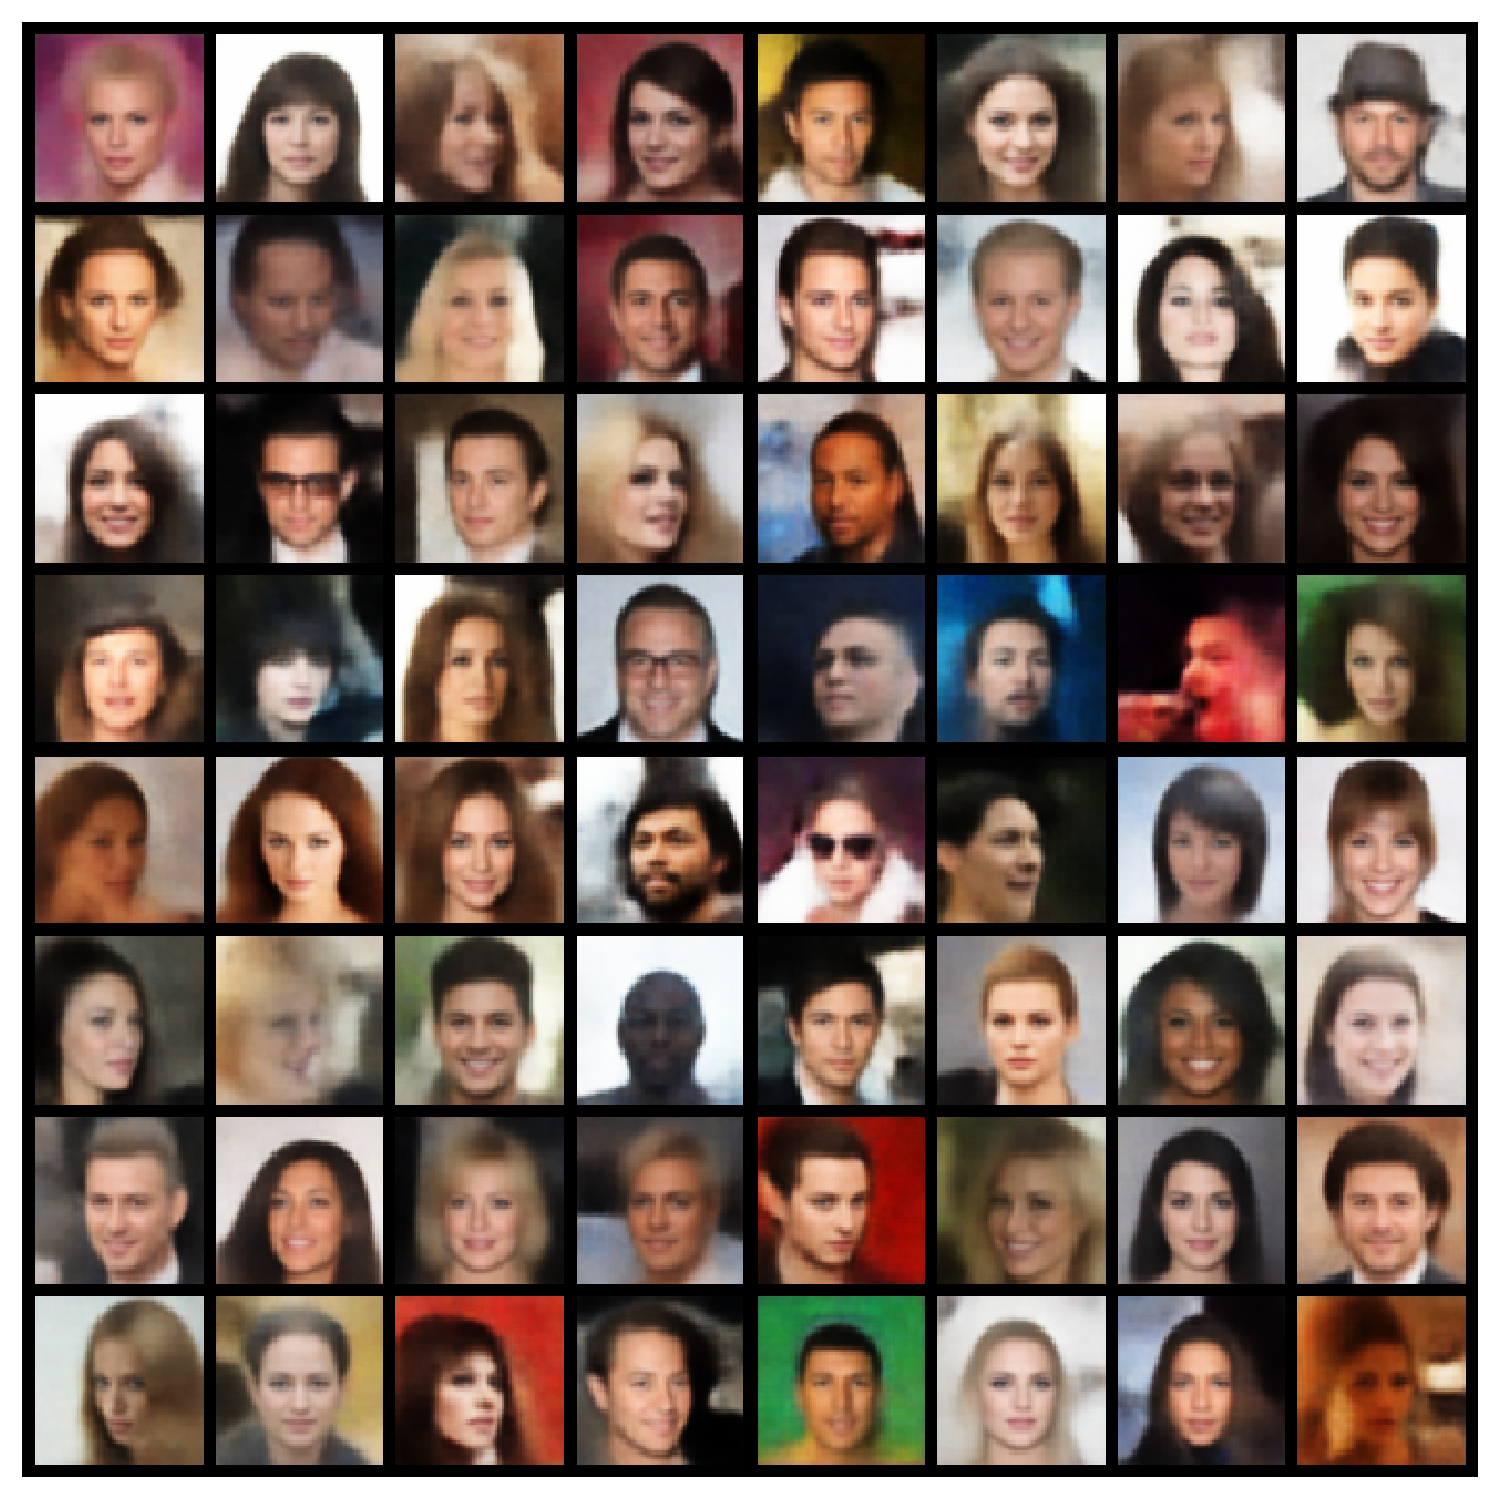
\includegraphics[width=.49\textwidth]{gfx/evaluation/celeba/fake-regular}
  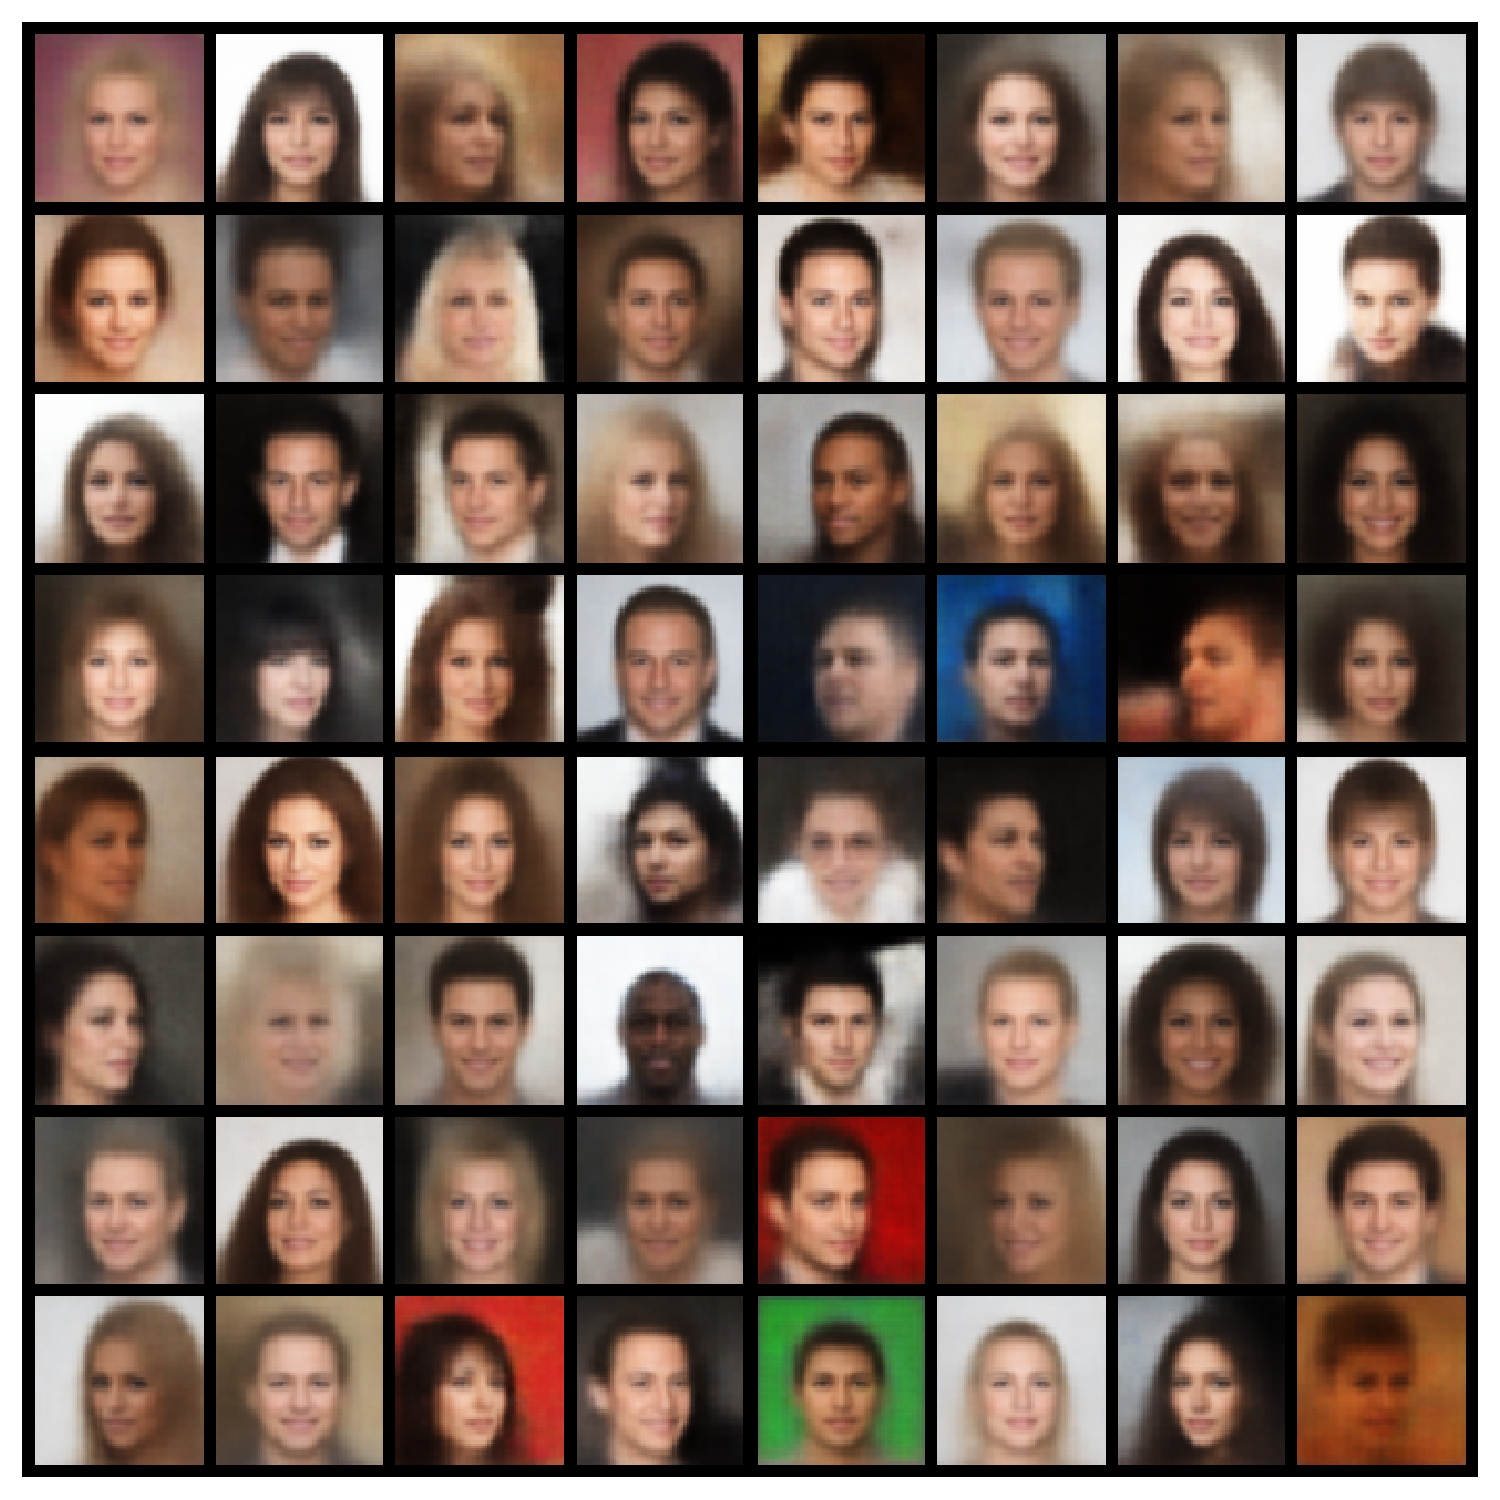
\includegraphics[width=.49\textwidth]{gfx/evaluation/celeba/fake-beta}
  \caption{CelebA - Originalbilder oben, Rekonstruktionen mit verschiedenen Werten für $\beta$ unten. $\beta_{norm}$ (links), $150 \cdot \beta_{norm}$ (rechts)}
  \label{fig:celeba_recon}
\end{figure}

In Abb. \ref{fig:celeba_disentangled} sind Interpolationen von beiden Modellen jeweils in einer Dimension zu sehen. Im oberen Bild stellt das interpolierte Merkmal eine Rotation von rechts nach links dar, im unteren Bild die Farbe der Haut. Man sieht, dass das Modell mit $\beta = 1$ Schwierigkeiten hat, die Merkmale "Hautfarbe" und "Lächeln" zu trennen. Dies ist bei dem Modell mit $\beta = 150$ nicht der Fall. Ein höherer $\beta$ Wert führt also zu Entwirrung von Merkmalen in den Dimensionen des Latent-Space. Erklären lässt sich das folgendermaßen (vgl. \cite{Higgins2017}): Durch den hoch gewichteten KL-Term wird die vom Encoder gebildete Normalverteilung Richtung Erwartungswert 0 und Varianz 1 gezwungen. Dies führt dazu, dass die Trennung von Merkmalen nun mehr über Dimensionen erfolgen muss. Daher sehen wir, dass verschiedene Dimensionen unterschiedliche Merkmale kontrollieren. Diese Repräsentation wird auch "Disentangled-Feature-Representation" genannt \cite{Higgins2017}. In Abb. \ref{fig:celeba_disentanglement_examples} sind weitere unabhängige Merkmale visualisiert.

\begin{figure}[hbt]
\centering
  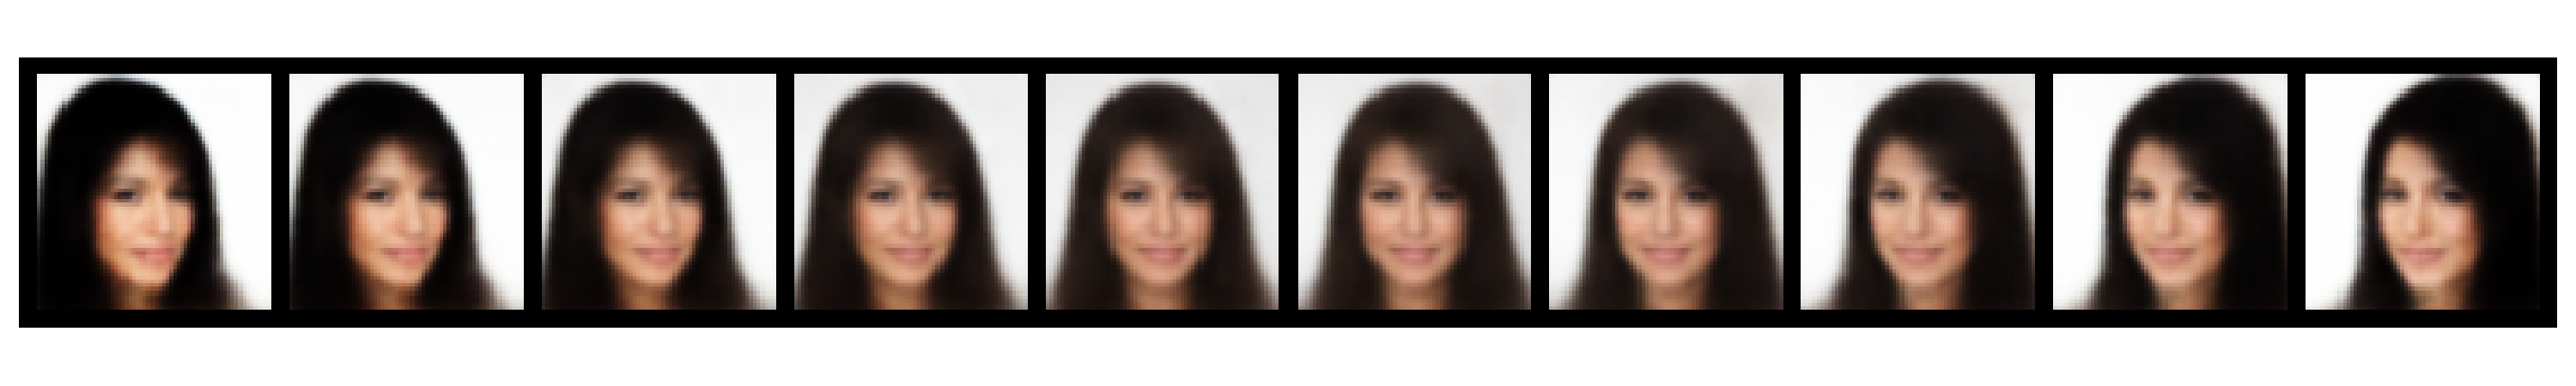
\includegraphics[width=.9\textwidth]{gfx/evaluation/celeba/CelebA-Rotation_1}
  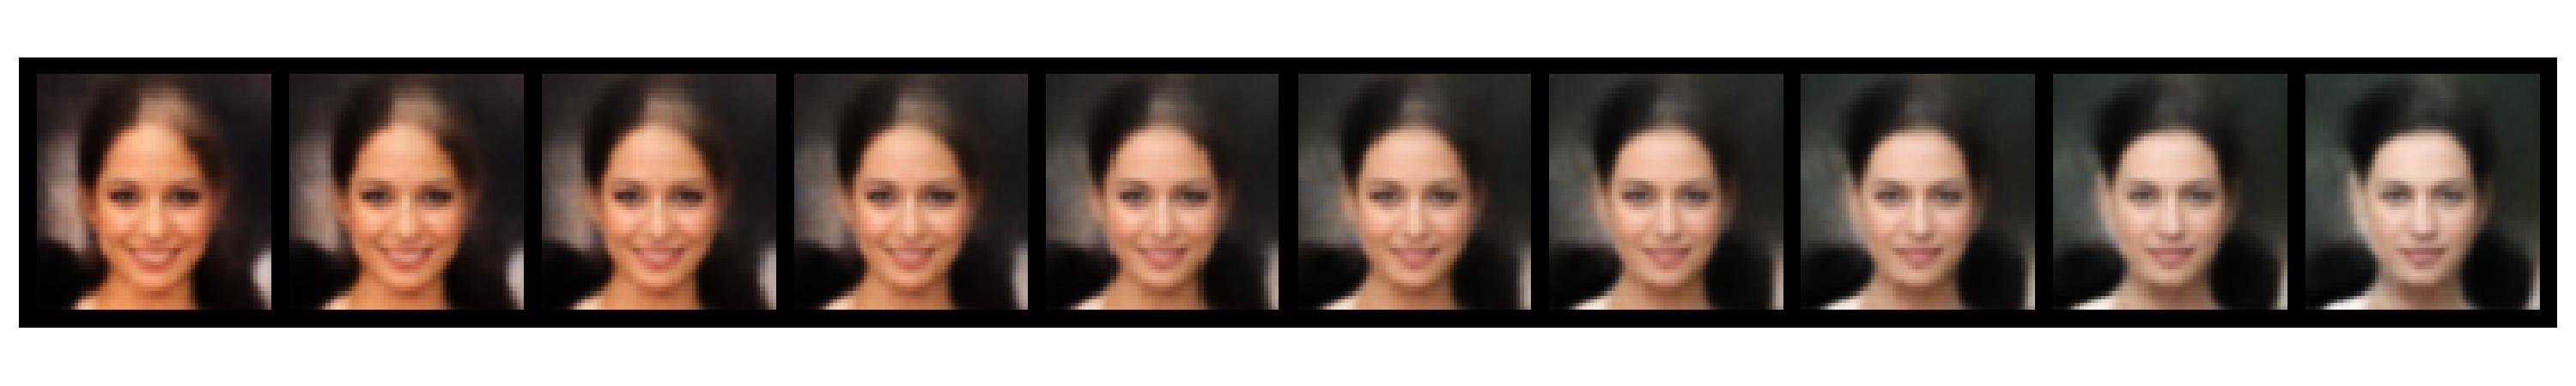
\includegraphics[width=.9\textwidth]{gfx/evaluation/celeba/regular-face-color}
  \caption{Sweep durch eine Dimension im Latent-Space für ein gegebenes Originalbeispiel (Die anderen Dimensionen sind fest). Oben zu sehen der VAE mit $\beta_{norm}$ für $\beta = 150$, unten $\beta_{norm}$ mit $\beta = 1$. Der höhere $\beta$ Wert erzielt eine bessere entkopplung der Merkmale. Unten zu sehen ist, dass das Merkmal "Hautfarbe" und "Lächeln" gekoppelt sind.}
  \label{fig:celeba_disentangled}
\end{figure}

\begin{figure}[H]
  \centering
  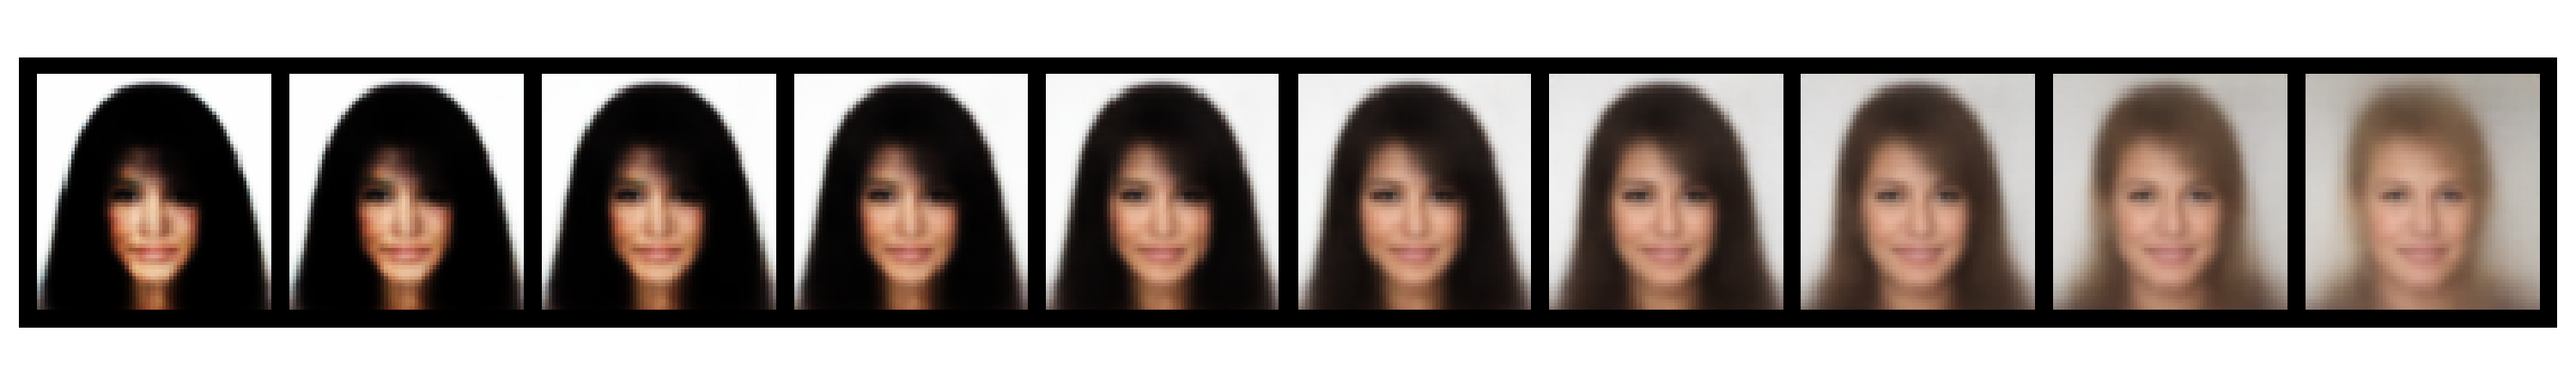
\includegraphics[width=.9\textwidth]{gfx/evaluation/celeba/CelebA-hair-color_1}
  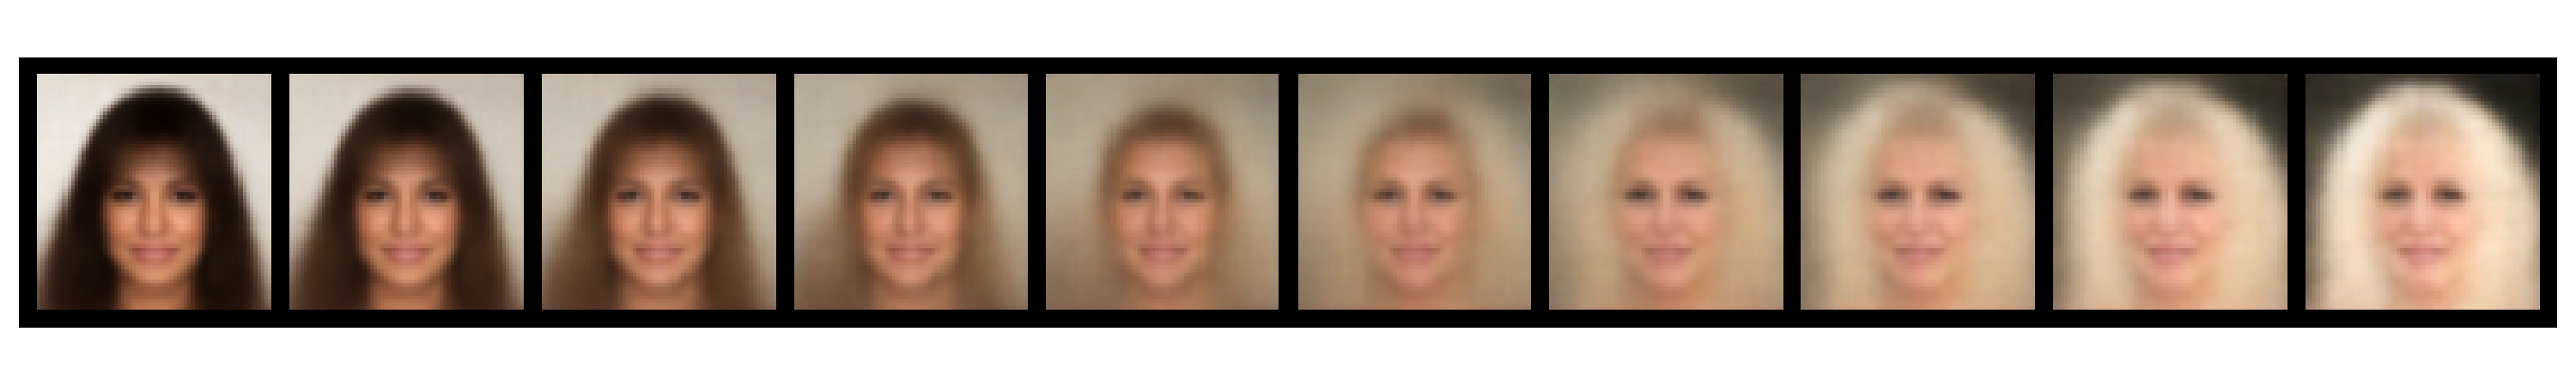
\includegraphics[width=.9\textwidth]{gfx/evaluation/celeba/CelebA-hair-color_3}
  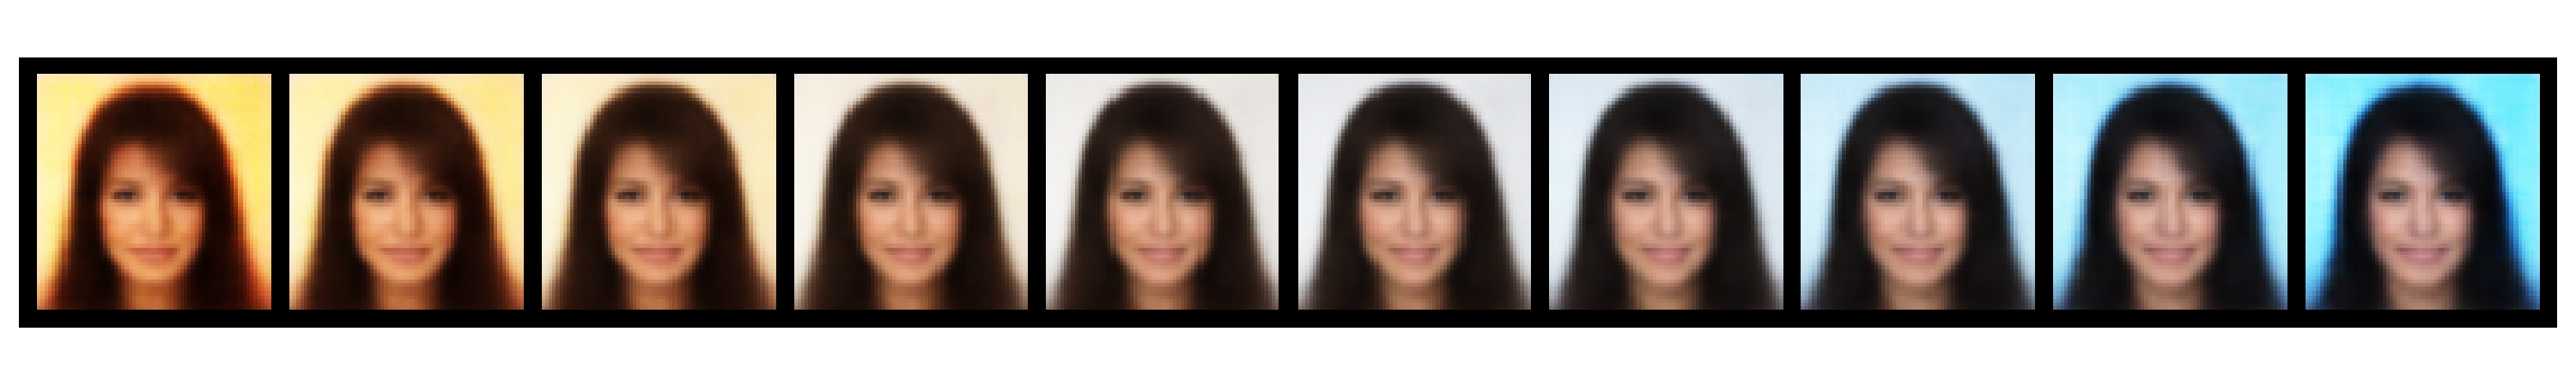
\includegraphics[width=.9\textwidth]{gfx/evaluation/celeba/CelebA-bg-color_1}
  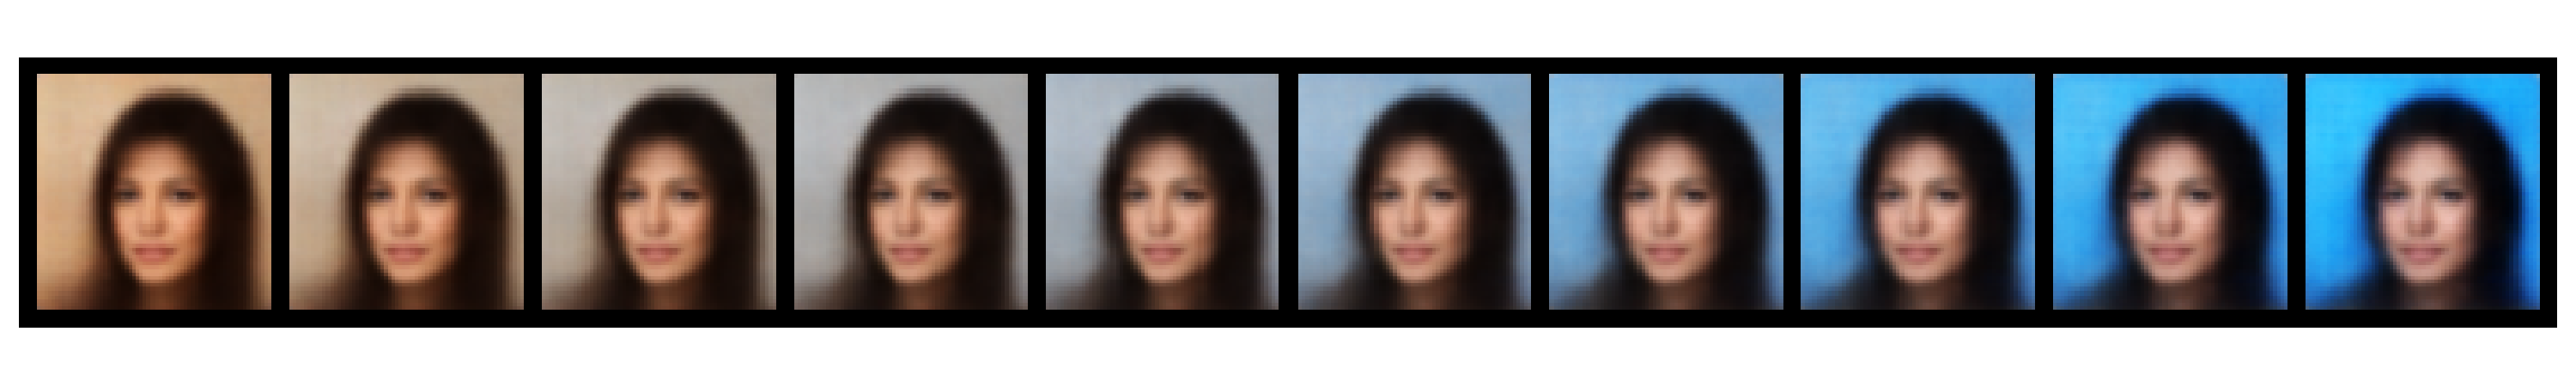
\includegraphics[width=.9\textwidth]{gfx/evaluation/celeba/CelebA-bg-color_3}
  \caption{Weitere entkoppelte Dimensionen des \textit{Disentangled}-VAE. Oben: Das Merkmal "Haarfarbe". Unten: Die Hintergrundfarbe.}
  \label{fig:celeba_disentanglement_examples}
\end{figure}



\section{Limitationen von VAE}
In den durchgeführten Experimenten ist aufgefallen, dass die Rekonstruktionen, welche der VAE erzeugt, unscharf sind. Dies betrifft vor allem den Hintergrund bei den Daten des CelebA Datensatzes. Für Datensätze, welche keine organischen Merkmale wie Gesichtszüge besitzen, ist dieser Effekt noch stärker ausgeprägt. Dies ist z.B. beim CIFAR-10 Datensatz der Fall (siehe Abb. \ref{fig:cifar10-bad-recon}).

\begin{figure}[H]
  \centering
  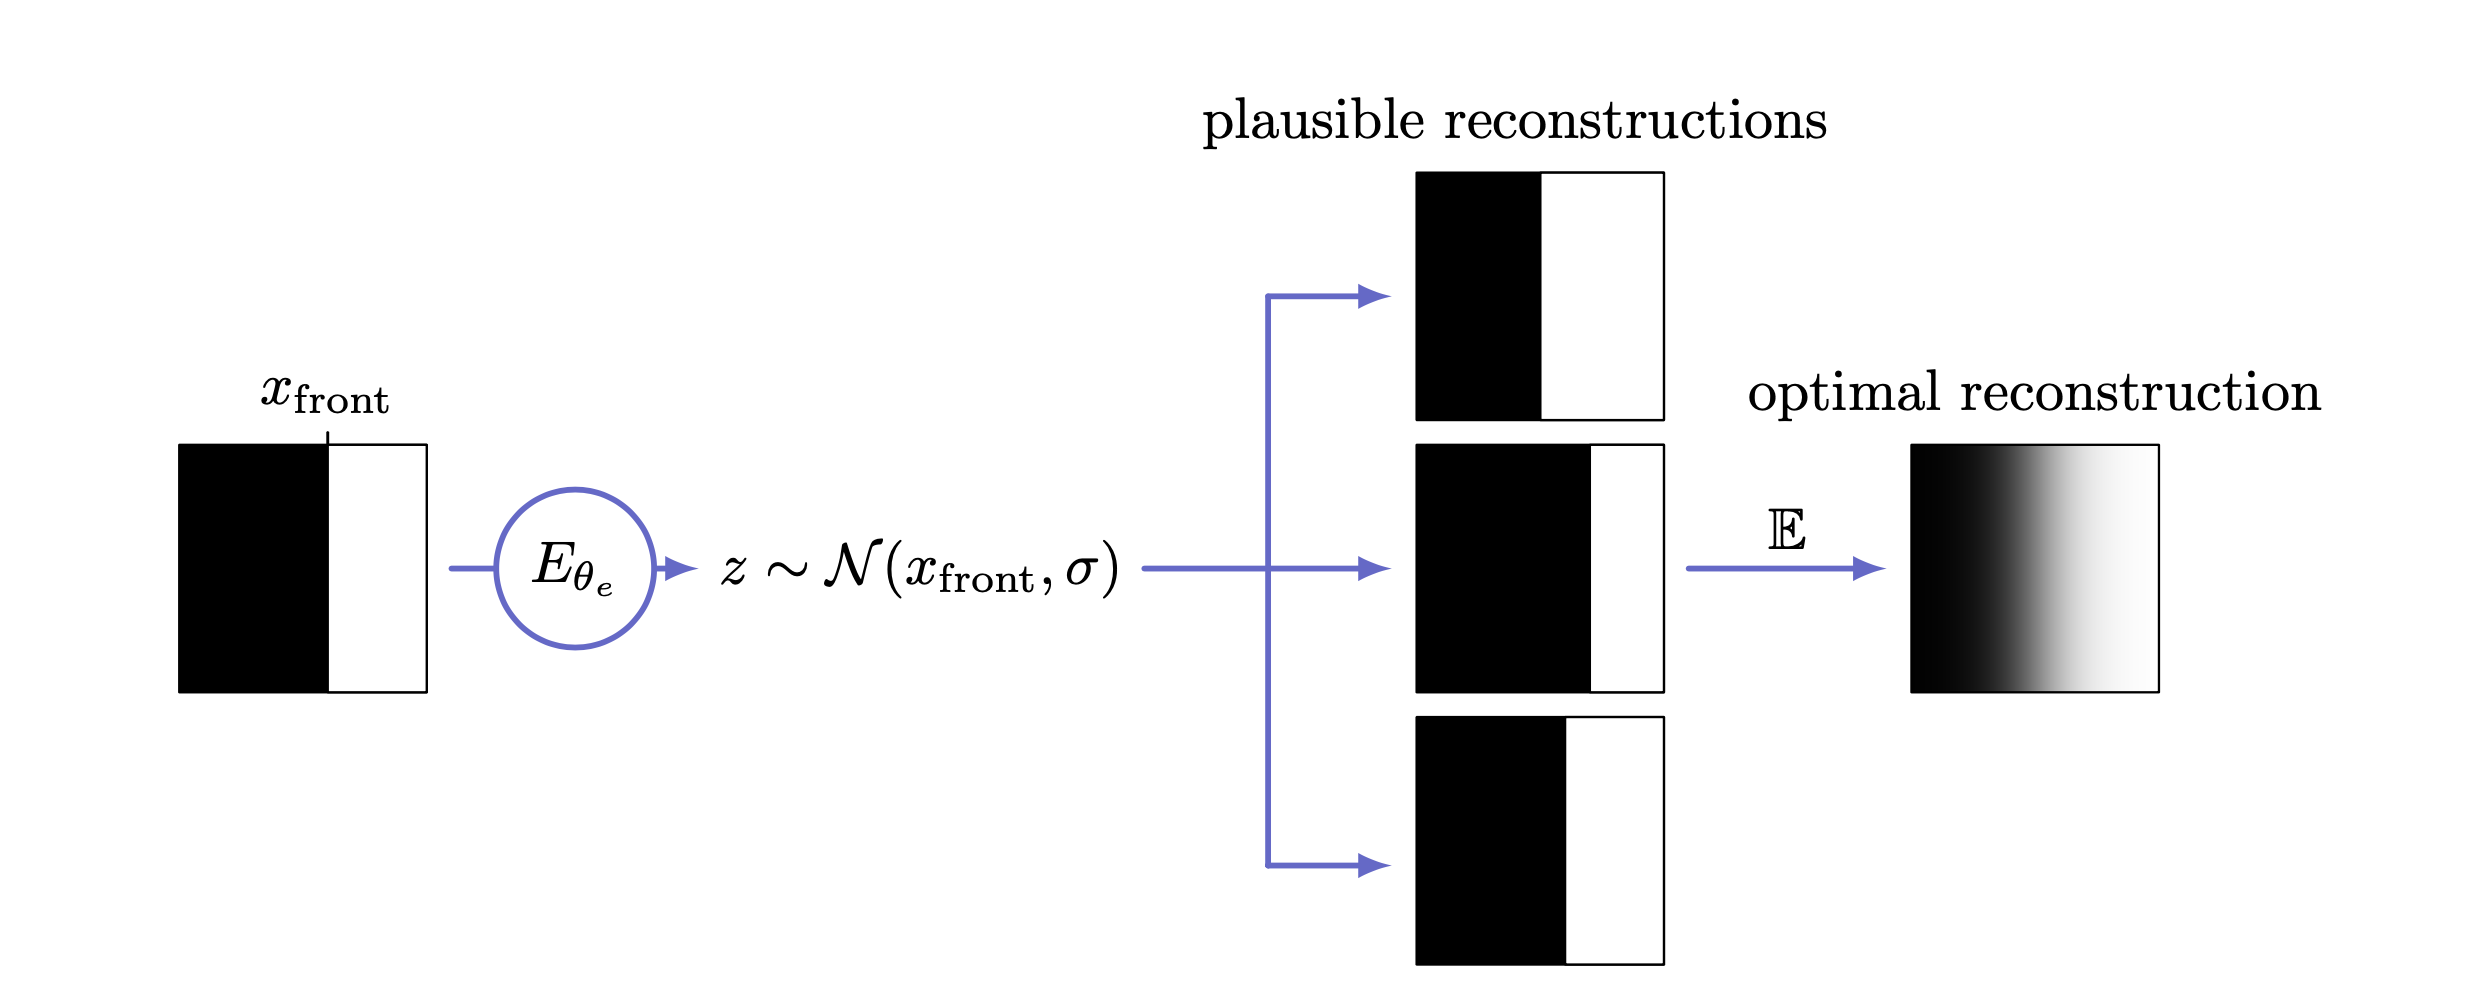
\includegraphics[width=.9\textwidth]{gfx/evaluation/recon_blur}
  \caption{Grund für die unscharfen Rekonstruktionen des VAEs ist die Modellierung der Ausgabe über eine Verteilung im Latent-Space. Damit sind mehrere Rekonstruktionen plausibel und ergeben eine unscharfe optimale Rekonstruktion.}
  \label{fig:blur_explained}
\end{figure}

Eine Erklärung für dieses Phänomen bei VAEs liefern \cite{Plumerault2020} (siehe Abb. \ref{fig:blur_explained}). Betrachtet wird eine Kante im Eingabebild $i$ und der Latent-Vektor $z$, welcher die Position $x_{front}$ der Kante beschreibt. Wenn nun
\[
Q_\phi(z \vert i) = \cN(x_{front}, \sigma)
\]
, dann ist die Verteilung der plausiblen Rekonstruktionen gegeben durch
\[
P_\theta(x_{front} \vert z) = \cN(z, \sigma)
\]. Die optimale Rekonstruktion des betrachteten Pixels ist durch den Erwartungswert über diese Verteilung gegeben, was einem weichen Übergang entspricht.

\begin{figure}[hbt]
  \centering
  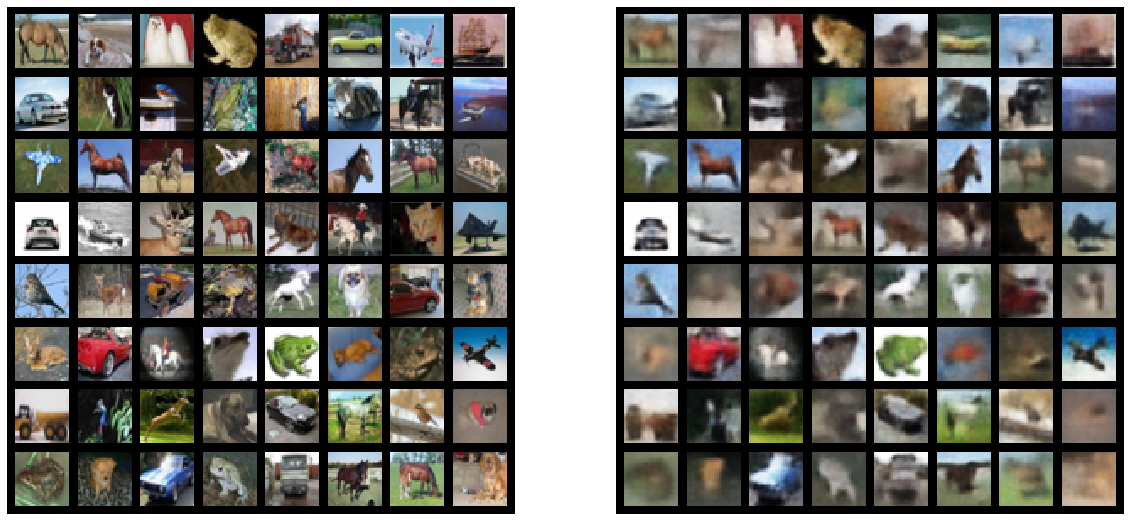
\includegraphics[width=\textwidth]{gfx/evaluation/cifar-10}
  \caption{Die Rekonstruktionen auf dem Datensatz CIFAR-10 sind besonders stark von der unschärfe des VAEs betroffen. In einigen Fällen ist die Klasse nicht mehr ableitbar.}
  \label{fig:cifar10-bad-recon}
\end{figure}



	
	% Conclusion
	\chapter{Fazit}
In dieser Arbeit wurden der Ansatz der Data Augmentation mit Variational Autoencodern auf unterschiedlichen Datensätzen untersucht. Die Verfahren wurden unter verschiedenen Szenarien evaluiert, welche in der Menge, Balance und Art der Daten variieren. Außerdem wurde die Repräsentation der Daten im Latent-Space durch die verschiedenen Modelle analysiert. Die wichtigsten Erkenntnisse werden im Folgenden zusammengefasst. \\

In der Evaluation konnten Schwierigkeiten des VAE Ansatzes im Umgang mit diskreten Attributen beobachtet werden. Dies machte diesen Ansatz auf numerischen Daten sehr Hyperparameter sensitiv. Außerdem wurden Probleme beim generieren neuer Daten festgestellt, da der Latent-Space eine kontinuierliche probabilistische Struktur hat. Die erzeugten Beispiele verbessern die Klassifikation daher nur geringfügig. Auf imbalancierten Datensätzen fiel die Verbesserung zusätzlich kleiner aus, da die stärker repräsentierte Klasse bessere Rekonstruktionen zur Folge hat. Im Vergleich zu den in der Arbeit von \cite{Moreno-Barea2020} genutzten generativen Methoden schneidet der VAE Ansatz schlechter ab. Im Few-Shot Szenario kann dagegen eine geringe, aber konsistente Verbesserung erreicht werden. Diese nimmt jedoch mit der Anzahl an original Beispielen ab.\\

Im Fall von Bilddaten zeigt der VAE eine , für die Modifikation von Bildern nützliche, Latent-Space Struktur. Insbesondere weiche Übergänge und organische Formen, wie Gesichtszüge, werden gut repräsentiert und erlauben Augmentierungen. Ein höher gewichteter KL-Term führte außerdem zu einer besseren Dekorrelation unterschiedlicher Merkmale in den Dimensionen des Latent-Spaces (\textit{Disentangled}-VAE). Im Allgemeinen sind die Rekonstruktionen des VAEs aber unscharf. Dies zeigt sich besonders bei harten Übergängen. 
Im Few-Shot Szenario zeigte sich auch hier eine konsistente Verbesserung des F-Scores. Außerdem konnte beobachtet werden, dass das selbst-überwachte Trainieren eines Single-VAEs bessere Ergebnisse erzielt, da wesentlich mehr Daten genutzt werden können.

\pagebreak

Zusammenfassend haben Variational Autoencoder ein großes Potenzial, reichen alleine jedoch nicht aus um herkömmliche Data Augmentation Techniken vollständig zu ersetzen. Das Verfahren ist im Allgemeinen äußerst Hyperparameter sensitiv. Die Encoder-Decoder Struktur bietet jedoch enorme Vorteile, da kontrollierbare Augmentationen im Latent-Space durchführbar sind. Mögliche Lösungsansätze für die Probleme und weitere Verbesserungen sind im folgenden Ausblick ausgeführt.

	
	% Outlook
	\chapter{Ausblick}
Es wurden bereits die Vorteile und Nachteile des VAE basierten Ansatzes der Data Augmentation vorgeführt. Im anschließenden Kapitel wird ein Ausblick über Weiterentwicklung der in dieser Arbeit vorgestellten Konzepte gegeben. \\

\section{Few-Shot Learning}
In der vorliegenden Arbeit wurde beobachtet, dass die verwendeten Augmentierungs Techniken, besonders im Few-Shot Szenario zu konsistenten Verbesserungen führten. Man beachte, dass diese Verbesserungen ausschließlich über Data Augmentation erzielt und keine Few-Shot Learning spezifischen Ansätze verwendet wurden. Eine vielversprechende Idee ist daher, die VAE basierte Data Augmentation mit \textit{State-of-the-Art} Few-Shot Learning Ansätzen, wie "Transfer-Learning" und "Meta-Learning", zu kombinieren.


%\section{Multi-Label Klassifikation}
%Die Multi-Label Klassifikationsaufgabe geht über den Fokus dieser Arbeit hinaus. Dennoch stellt sich die Frage, inwiefern die Klassifikation verbessert werden kann, wenn die Daten eines Distentangled-VAE hinzugenommen werden. Außerdem repräsentieren die Dimensionen des Latent-Space nicht alle gelernten Merkmale. \cite{Klys2018} liefern einen Ansatz, um besser Subräume im Latent-Space zu finden, die Attributen im Datensatz entsprechen.
\section{Weitere VAE Modelle}
\subsection{Denoising und Conditional VAE}
Für die Anwendung von VAE Modellen auf den numerischen Daten des PROBEN1 Datensatzes, wurden von \cite{Moreno-Barea2020} zwei Weiterentwicklungen vorgestellt: Der Denoising-VAE (DVAE) und der Conditional-VAE (CVAE). Der DVAE hat dieselbe Funktionsweise wie schon der in Abschnitt \ref{sec:dae} angeführte Denoising Autoencoder. Das Eingabebeispiel $x$ wird durch eine modifizierte Variante $\tilde{x}$ ersetzt. Der CVAE gibt dem VAE zusätzlich zum gesampelten $z$ die Klassen Information $y$ mit. Die Ausgabeverteilung des Encoders und Decoders hängt somit jeweils auch von der Klasse des gesampelten Latent-Vektors ab. Die Fehlerfunktion von DVAE und CAE haben folgende Form:
\begin{align}
  \cL_{\textit{DVAE}} &= \bE \left[\log P_\theta(x \vert z) - \cD_{KL}\left[Q_\phi(z \vert \tilde{x}) \| \cN(0, 1)\right] \right] \\[6pt]
  \cL_{\textit{CVAE}} &= \bE \left[\log P_\theta(x \vert z, y) - \cD_{KL}\left[Q_\phi(z \vert x, y) \| \cN(0, 1)\right] \right]
\end{align}


\subsection{VAE-GAN}
\cite{Larsen2016} schlagen in ihrer Arbeit eine Kombination des VAE Modells mit einem Generative-Adversarial-Network (GAN) vor. GANs erzeugen wesentlich schärfere Bilder, haben aber keinen Encoder. Dies hat zur Folge, dass sie weniger Kontrolle über die Rekonstruktionen bieten, da keine Manipulationen im Latent-Space möglich sind. Das vorgeschlagene VAE-GAN Modell kombiniert den Encoder des VAEs mit der Generator-Discriminator Architektur des GANs, indem der Decoder durch den Generator und Discriminator ersetzt wird (siehe Abb. \ref{fig:vae_gan}). VAE-GANs haben die gleichen Latent-Space Eigenschaften wie VAEs, erzeugen aber wesentlich schärfere Bilder, wie in Abb. \ref{fig:vae_gan_reconstruction} zu sehen ist. Damit führen die Autoren die Vorteile dieser beiden generativen Ansätze in einem Modell zusammen.

%Ein GAN besteht aus zwei Netzwerken: Einem Generator und ein Discriminator (siehe auch \cite{goodfellow2014generative}. Der Generator bildet Elemente $z$ aus dem Latent-Space auf ein $\hat{x}$ in den Raum der Daten ab. Der Discriminator bewertet, ob das erzeugte Beispiel ein "echtes" Trainingsbeispiel oder ein generiertes Beispiel ist. Beide Netzwerke optimieren sich gegenseitig über folgende Fehlerfunktion:
%\begin{equation}
%  \cL_{GAN} = \log Dis(x) + \log(1 - Dis(Gen(z)),
%\end{equation}
%mit $x \sim D$ Datensatz und $z \sim P(z)$.\\

\begin{figure}[hbt]
\centering
  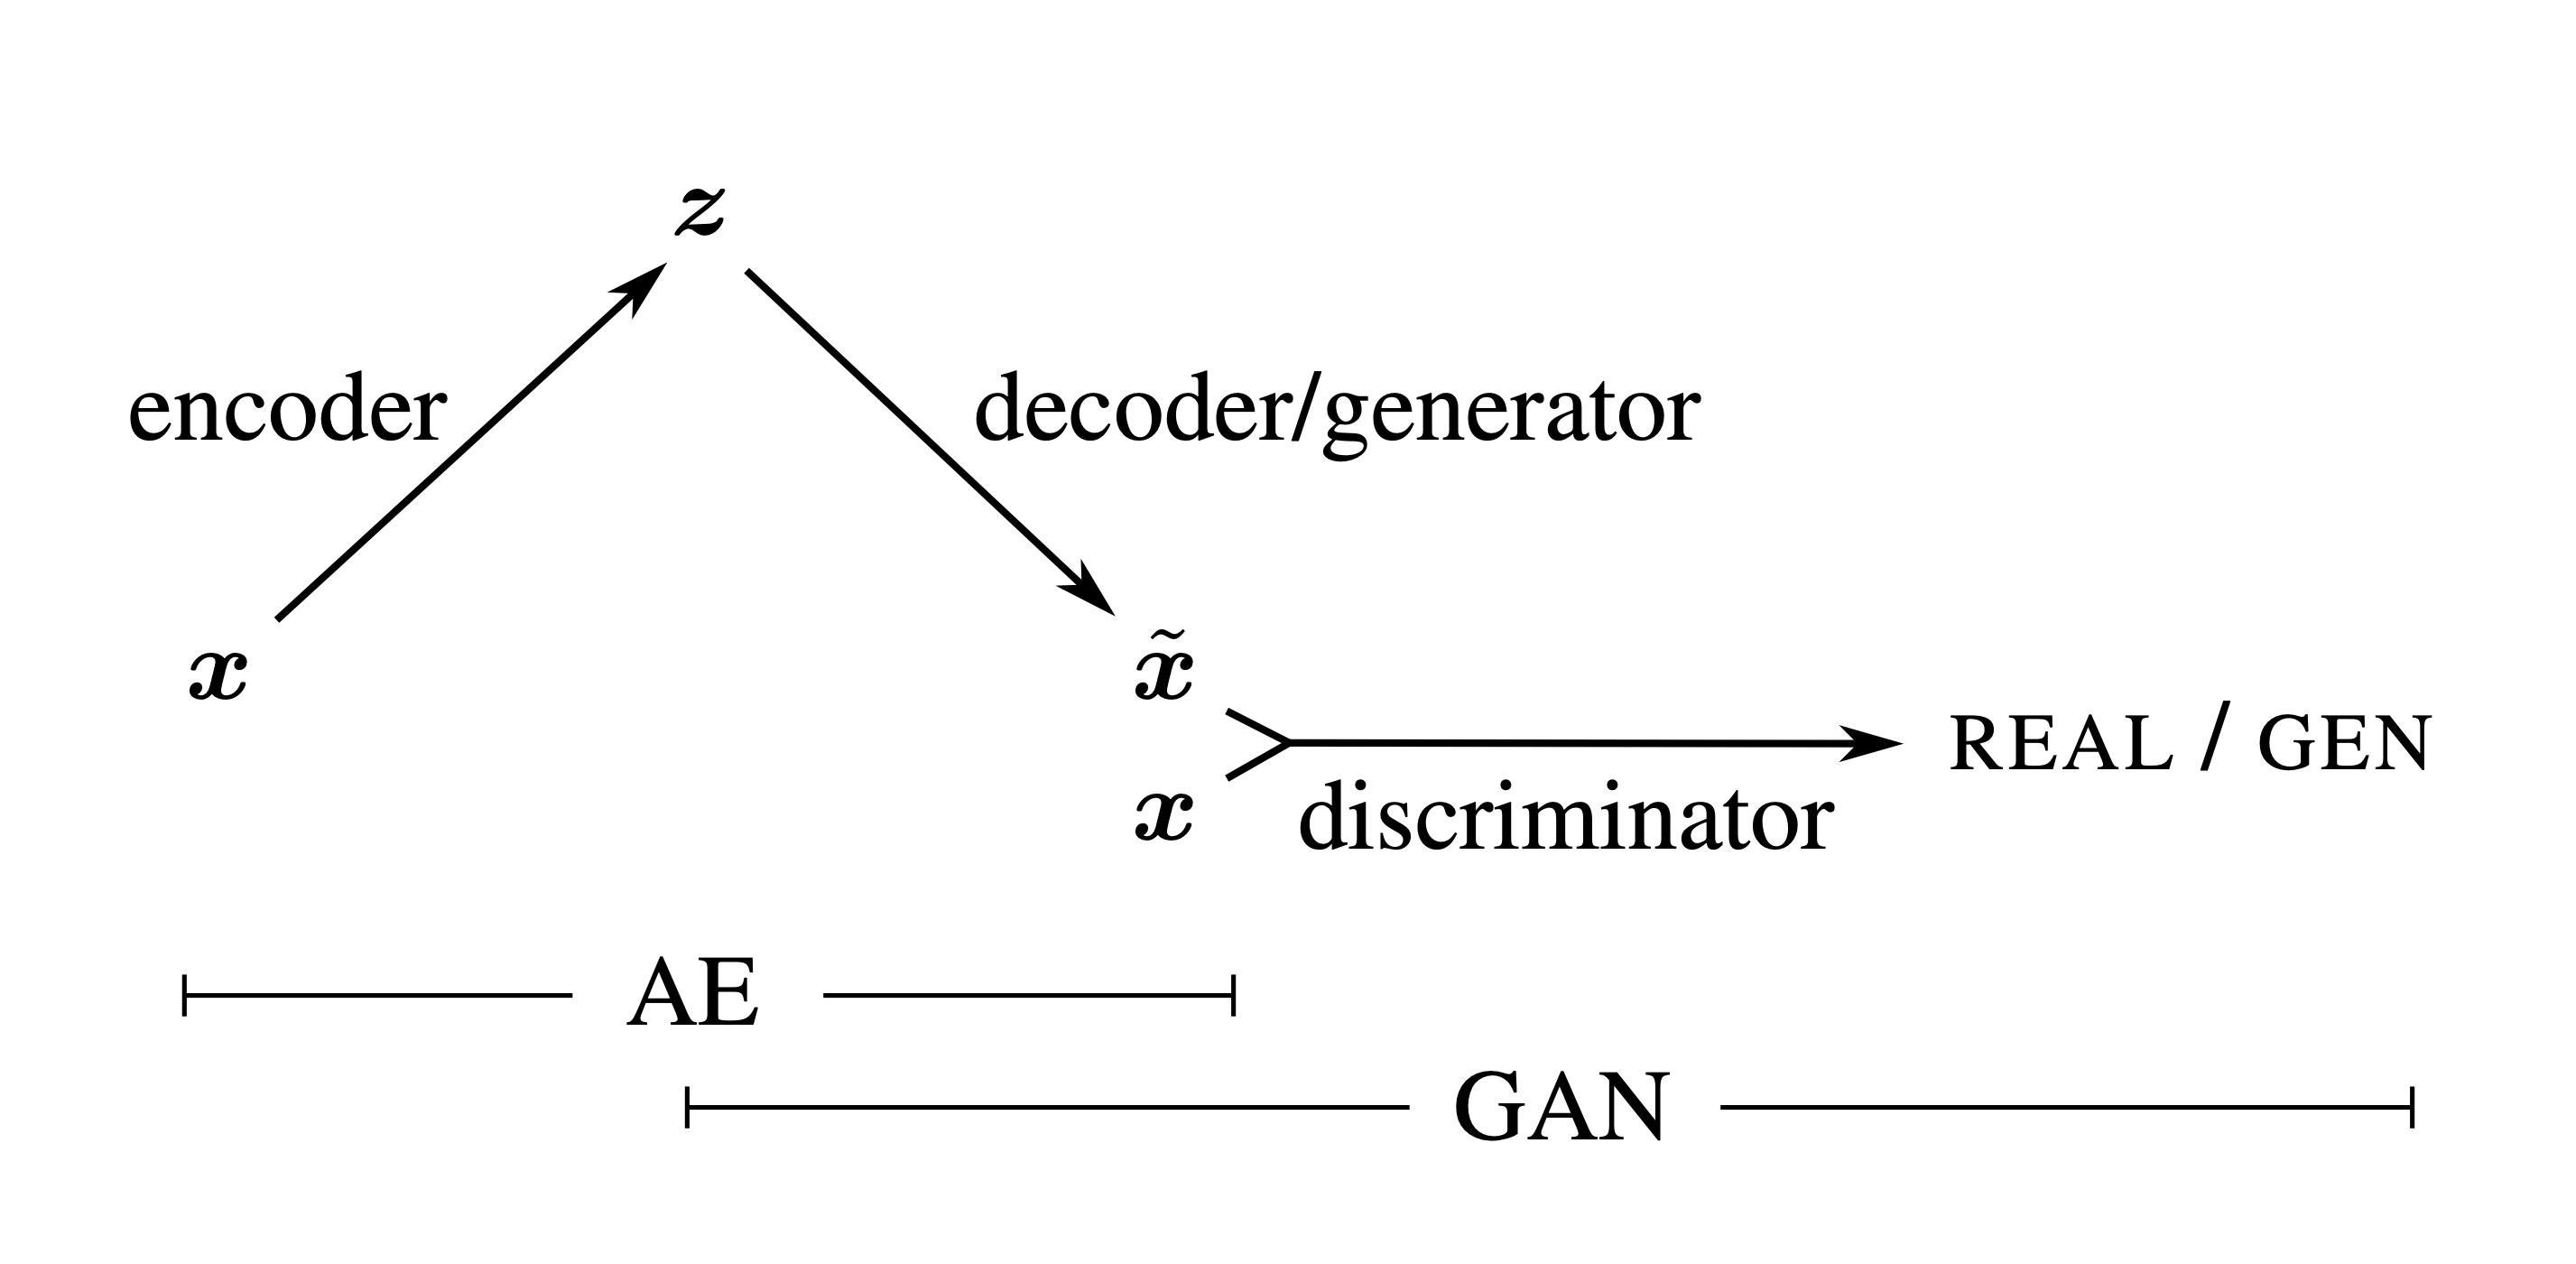
\includegraphics[width=.7\textwidth]{gfx/outlook/vae_gan}
  \caption{Das VAE-GAN Modell. Der Decoder des VAEs wird durch den Generator und den Discriminator ersetzt. Abbildung entnommen aus \cite{Larsen2016}}
  \label{fig:vae_gan}
\end{figure}

\begin{figure}[hbt]
\centering
  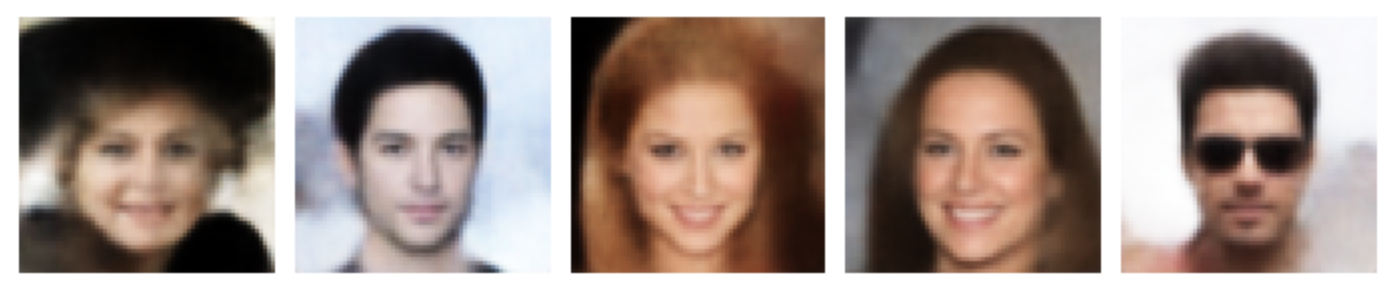
\includegraphics[width=.7\textwidth]{gfx/outlook/ours}
  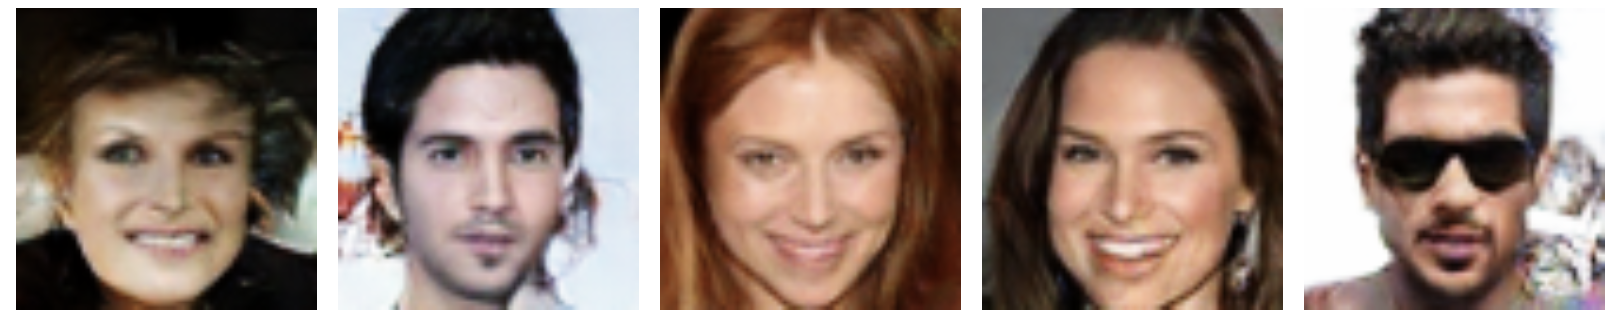
\includegraphics[width=.7\textwidth]{gfx/outlook/vae_gan_reconstruction}
  \caption{Die Rekonstruktionen unseres VAE Modells (oben). Die Rekonstruktionen des VAE-GAN Modells (unten) (VAE-GAN Bilder entnommen aus \cite{Larsen2016})}
  \label{fig:vae_gan_reconstruction}
\end{figure}

	
	% Workaround: 
	% The backmatter deactivates chapter numbering for the appendices which are 
	% supposed to appear in the backmatter _after_ the bibliography. This makes 
	% referencing the appendices a hassle. A workaround is to put the
	% backmatter, bibilography, and lists-of in a LaTeX group using \begingroup 
	\begingroup 
	
	\backmatter
		
	\printbibliography[heading=bibintoc]
	
	\listoffigures
	
	\listoftables
	
	\endgroup 
	% End of Workaround 
	
	\appendix	
	
\end{document}
